% !TeX encoding=utf8
% !TeX program = pdflatex
% !TeX spellcheck = de_CH_frami

%% Bug fixes and other packages to be loaded before the class
\RequirePackage[l2tabu, orthodox]{nag} % check for mistakes in the code
\RequirePackage{fix-cm} % permit Computer Modern fonts at arbitrary sizes.
%
%% Document Class (Koma Script) -----------------------------------------
%% Doc: scrguien.pdf
\documentclass[%
   %draft=true,     % draft mode (no images, layout errors shown)
   draft=false,     % final mode 
%%% --- Paper Settings ---
   paper=a4,% [Todo: add alternatives]
   paper=portrait, % landscape
   pagesize=auto, % driver
%%% --- Base Font Size ---
   fontsize=11pt,%
%%% --- Koma Script Version ---
   version=last, %
%%% --- Global Package Options ---
   ngerman, % language (passed to babel and other packages)
            % (ngerman, english, french, ...)
]{scrbook} % Classes: scrartcl, scrreprt, scrbook

% ~~~~~~~~~~~~~~~~~~~~~~~~~~~~~~~~~~~~~~~~~~~~~~~~~~~~~~~~~~~~~~~~~~~~~~~~
% Must be loaded first!
% ~~~~~~~~~~~~~~~~~~~~~~~~~~~~~~~~~~~~~~~~~~~~~~~~~~~~~~~~~~~~~~~~~~~~~~~~
% packages to allow more \write outputs
% Description: Package scrwfile provides a general change of the LaTeX kernel, 
%              that solve problems with the 
%              error "no room for a new \write"
% Incompatible: titletoc (bot redefine the LaTeX kernel and are incompatible by design)
% Doc: scrguien.pdf
%
%% If titletoc is not required, the usage of this package is recommended!
% \usepackage{scrwfile}

% Description: This package is meant to be a solution for the 
%              error "no room for a new \write"
% Note: it is less efficent than scrwfile, but the best alternative
% Doc: morewrites.pdf
\usepackage{morewrites}


% Description: see http://www.tex.ac.uk/cgi-bin/texfaq2html?label=noroom
%   short summery: The e-TeX extensions do not help with the 
%                  "no room for a new \write" problem, but in other cases
%                  of "no room for a new <thing> "
\usepackage{etex} 
\reserveinserts{28}


% packages required for the template
\usepackage{codesection}
\usepackage{templatetools}
% ~~~~~~~~~~~~~~~~~~~~~~~~~~~~~~~~~~~~~~~~~~~~~~~~~~~~~~~~~~~~~~~~~~~~~~~~
% encoding
% ~~~~~~~~~~~~~~~~~~~~~~~~~~~~~~~~~~~~~~~~~~~~~~~~~~~~~~~~~~~~~~~~~~~~~~~~

% automatic selection of encoding
% insert chars for umlaut a and sz
\usepackage{selinput}
\SelectInputMappings{adieresis={ä},germandbls={ß},Euro={€}} 

% Encoding of _files and directories_
% (ensures that any file can be loaded without problems)
\usepackage[%
   extendedchars, encoding, multidot, space,
   filenameencoding=latin1, % Windows XP, Vista, 7
   % filenameencoding=utf8,   % Linux, OS X
]{grffile}

% ~~~~~~~~~~~~~~~~~~~~~~~~~~~~~~~~~~~~~~~~~~~~~~~~~~~~~~~~~~~~~~~~~~~~~~~~
% preamble
% ~~~~~~~~~~~~~~~~~~~~~~~~~~~~~~~~~~~~~~~~~~~~~~~~~~~~~~~~~~~~~~~~~~~~~~~~

%% select/load fonts
% ~~~~~~~~~~~~~~~~~~~~~~~~~~~~~~~~~~~~~~~~~~~~~~~~~~~~~~~~~~~~~~~~~~~~~~~~
% Fonts Fonts Fonts
% ~~~~~~~~~~~~~~~~~~~~~~~~~~~~~~~~~~~~~~~~~~~~~~~~~~~~~~~~~~~~~~~~~~~~~~~~

% Make PDF files searchable and copyable
% load before: fontenc
\usepackage{cmap} 

% T1 Schrift Encoding
\usepackage[T1]{fontenc} 

% Description: Additional Symbols (Text Companion font extension)
% Doc: encguide.pdf
\usepackage{textcomp}   

% DO NOT LOAD ae Package as a font !

%% ==== Font Families / Font Combinations  (Sans + Serif) ================

%% - Latin Modern (LaTeX Standard)
\usepackage{lmodern}
%% sans math, use with '\mathversion{sans}'
\IfPackageLoaded{lmodern}{\DeclareMathVersion{sans}
% Math letters from Latin Modern Sans
\SetSymbolFont{letters}{sans}{OML}{cmbr}{m}{it}
% Math operators
\SetSymbolFont{operators}{sans}{OT1}{lmss}{m}{n}
% Math symbols
\SetSymbolFont{symbols}{sans}{OMS}{lmsy}{m}{n}
% Large symbols
\SetMathAlphabet{\mathrm}{sans}{OT1}{lmr}{m}{n}
\SetMathAlphabet{\mathsf}{sans}{OT1}{lmss}{m}{n}
\SetMathAlphabet{\mathit}{sans}{OT1}{lmr}{m}{it}
}

%% -------------------
%
%% - Times, Helvetica, Courier (Word Standard...)
%\usepackage{mathptmx}                 %% --- Times (incl math)
%\usepackage[scaled=.90]{helvet}       %% --- Helvetica (Arial)
%\usepackage{courier}                  %% --- Courier
%% -------------------
%%
%% - Palantino , Helvetica, Courier
%\usepackage{mathpazo}                 %% --- Palantino (incl math)
%\usepackage[scaled=.95]{helvet}       %% --- Helvetica (Arial)
%\usepackage{courier}                  %% --- Courier
%% -------------------
%
%% - Charter, Bera Sans
%\usepackage{charter}\linespread{1.05} %% --- Charter
%\renewcommand{\sfdefault}{fvs}        %% --- Bera Sans
%\usepackage[charter]{mathdesign}      %% --- Charter (Math)
%\usepackage[scaled=0.85]{luximono}    %% --- Luxi Mono (Typewriter)
%% Note: There is a better Charter font by Linotype 
%%       called 'ITC Charter'
%% -------------------

%% - URW Garamond
%\renewcommand{\rmdefault}{ugm}         %% --- URW Garamond
%\renewcommand{\sfdefault}{fvs}         %% --- Bera Sans
%%%\usepackage[small]{eulervm}            %% --- EulerVM (MATH)
%\usepackage[garamond]{mathdesign}    %% --- Garamond (Math)
%\usepackage[scaled=0.85]{luximono}    %% --- Luxi Mono (Typewriter)
%% Note:  If you can efford it, combine with commercial 
%%        sans fonts like: Syntax, Frutiger or Thesis 
%%        (but then also use the commercial Garamond ...)
%% -------------------


%%%% =========== Typewriter =============

%\usepackage{courier}                   %% --- Courier
%\renewcommand{\ttdefault}{cmtl}        %% --- CmBright Typewriter Font
%\usepackage[scaled=0.9]{luximono}      %% --- Luxi Mono (Typewriter)
%\usepackage{ulgothic}                  %% --- Letter Gothic 

%%%% =========== Math fonts ================

%% Recommanded to use with fonts: Aldus, Garamond, Melior, Sabon
%\usepackage[                           %% --- EulerVM (MATH)
%   small,       %for smaller Fonts
%  euler-digits % digits in euler fonts style
%]{eulervm}

%% combine with utopia, garamond or charter font
%\usepackage[
%%   utopia,
%%   garamond,
%%   charter
%]{mathdesign}



%%% ==== Font Families / Font Combinations  (Sans + Serif) ==========

%% - MininPro/MyriadPro
%% load after textcomp, amsmath and MnSymbol
\IfFileExists{MinionPro.sty}{
%
\ExecuteAfterPackage{amsmath}{
% Minion Pro
\usepackage[%
%%% Font selection
  %smallfamily, % (std) use only regular and bold face
  medfamily,    % use semibold face in addition to smallfamily
  %fullfamily,  % use medium face in addition to medfamily
  noopticals,   % (std) use only the optical size Text
  %opticals     % use the optical sizes Caption, Text, Subhead, and Display
  %slides,      % use only the optical size Caption (useful for slides)
  normalsize,   % (std) adapt optical sizes to the normal font size 
  %nonormalsize,% use static settings for the optical sizes
  % onlytext,   % only change the text fonts
  % onlymath,   % only change the math fonts
%%% Figure selection
  % textosf,    % use text figures in text mode
  % mathosf,    % use text figures in math mode
  % osf,        % (std) use text figures in text and math mode
  % textlf,     % use lining figures in text mode
  % mathlf,     % use lining figures in math mode
  lf,,          % use lining figures in text and math mode
  mathtabular,  % use tabular figures in math mode
%%% Miscellaneous options
  % scaled=1.0, % scale the font size by <factor>
%  minionint,    % take the integral symbols from MyriadPro, not from MnSymbol
]{MinionPro}
} % end of ExecuteAfter
%
% file not found:
}{\PackageWarning{template}{File 'MinionPro.sty' not found!\MessageBreak}{}}  %% --- MinionPro
%\IfFileExists{MyriadPro.sty}{
% load after textcomp, amsmath and MnSymbol
\ExecuteAfterPackage{amsmath}{
%% Myriad Math Fonts 
%\usepackage[onlysansmath]{MdSymbol}
%
\usepackage[%
%%% Font selection
  % smallfamily, % (std) use only regular and bold face
  medfamily,   % use semibold face in addition to smallfamily
  onlytext,    % only change the text fonts
  % onlymath   % only change the math fonts
  sansmath,     % provide math version sans and sansbold 
%%% Figure selection
  % textosf, % use text figures in text mode
  % mathosf, % use text figures in math mode
  % osf,       % (std) use text figures in text and math mode
  textlf,  % use lining figures in text mode
  mathlf,    % use lining figures in math mode
  % lf,      % use lining figures in text and math mode
  mathtabular, % use tabular figures in math mode
%%% Miscellaneous options
  % scaled=1.0, % scale the font size by <factor>
]{MyriadPro}[2012/01/07 v0.1c]

} % end of ExecuteAfter
%
% file not found:
}{\PackageWarning{template}{File 'MyriadPro.sty' not found!\MessageBreak}{}}

% set bold to medium bold by default
\renewcommand{\bfdefault}{sb}

%% If you want to use MyriadPro as your mainfont:
% \renewcommand{\familydefault}{\sfdefault}  %% --- MyriadPro
%\usepackage[scaled=0.85]{luximono} %% --- Luxi Mono (Typewriter)
%% -------------------

%% - Minion / Myriad
%\renewcommand{\rmdefault}{pmnx}   % Minion
%%\renewcommand{\rmdefault}{pmnj}  % Minion ()oldstyle digits)
%\renewcommand{\sfdefault}{pmy}    % Myriad
%% Minion Math Fonts 
%\ExecuteAfterPackage{amsmath}{\usepackage{MnSymbol}}
%% -------------------

%% ===== serif ( commercial fonts ) ================================

%% --- Adobe Aldus
%\renewcommand{\rmdefault}{pasx}
%\renewcommand{\rmdefault}{pasj} %%oldstyle digits
% math recommended: \usepackage[small]{eulervm}

%% --- Adobe Garamond
%\usepackage[garamond]{mathdesign}
%\usepackage[%
%   osf,        % oldstyle digits
%   scaled=1.05 %appropriate in many cases
%]{xagaramon}


% math recommended: \usepackage{eulervm}

%% --- Adobe Stempel Garamond
%\renewcommand{\rmdefault}{pegx}
%\renewcommand{\rmdefault}{pegj} %%oldstyle digits
%\usepackage[garamond]{mathdesign}

%% --- Adobe Melior
%\renewcommand{\rmdefault}{pml}
% math recommended: %\usepackage{eulervm}

%% --- Adobe Minion
%\renewcommand{\rmdefault}{pmnx}
%\renewcommand{\rmdefault}{pmnj} %oldstyle digits
% math recommended: \usepackage[small]{eulervm} or \usepackage{mathpmnt} % commercial
%\usepackage{MnSymbol}
%\renewcommand{\bfdefault}{sb}

%% --- Adobe Sabon
%\renewcommand{\rmdefault}{psbx}
%\renewcommand{\rmdefault}{psbj} %oldstyle digits
% math recommended: \usepackage{eulervm}

%% --- Adobe Times
% math recommended: \usepackage{mathptmx} % load first !
%\renewcommand{\rmdefault}{ptmx}
%\renewcommand{\rmdefault}{ptmj} %oldstyle digits

%% --- Linotype ITC Charter
%\renewcommand{\rmdefault}{lch}
%\usepackage[charter]{mathdesign}


%% --- Linotype Meridien
%\renewcommand{\rmdefault}{lmd}

%%% ===== sans serif (commercial fonts ) ============================

%% --- Adobe Frutiger
%\usepackage[
%   scaled=0.90
%]{frutiger}

%% --- Adobe Futura (=Linotype FuturaLT) : Sans Serif
%\usepackage[
%   scaled=0.94  % appropriate in many cases
%]{futura}

%% --- Adobe Gill Sans : Sans Serif
%\usepackage{gillsans}

%% -- Adobe Myriad  : Sans Serif
%\renewcommand{\sfdefault}{pmy}
%\renewcommand{\sfdefault}{pmyc} %% condensed Font

%% --- Syntax : sans serif font
%\usepackage[
%   scaled
%]{asyntax}

%% --- Adobe Optima : Semi Sans Serif
%\usepackage[
%   medium %darker medium weight fonts
%]{optima}

%% --- Linotype ITC Officina Sans
%\renewcommand{\sfdefault}{lo9}


%% load packages
% !TeX encoding=utf8
% !TeX program = pdflatex
% !TeX spellcheck = de_CH_frami

%% -- package section selections -->
\DefineCodeSection[true]{PackagesBase}
\DefineCodeSection[true]{PackagesBugfixes}
\DefineCodeSection[true]{PackagesFonts}
\DefineCodeSection[true]{PackagesDiagrams}
\DefineCodeSection[true]{PackagesMath}
\DefineCodeSection[true]{PackagesScience}
\DefineCodeSection[true]{PackagesSymbols}
\DefineCodeSection[true]{PackagesTables}
\DefineCodeSection[true]{PackagesText}
\DefineCodeSection[true]{PackagesQuotes}
\DefineCodeSection[true]{PackagesCitation}
\DefineCodeSection[true]{PackagesFigures}
\DefineCodeSection[true]{PackagesCaptions}
\DefineCodeSection[true]{PackagesIndexes}
\DefineCodeSection[true]{PackagesMisc}
\DefineCodeSection[true]{PackagesVerbatim}
\DefineCodeSection[true]{PackagesFancy}
\DefineCodeSection[true]{PackagesLayout}
\DefineCodeSection[true]{PackagesHeadFoot}
\DefineCodeSection[true]{PackagesHeadings}
\DefineCodeSection[true]{PackagesTOC}
\DefineCodeSection[true]{PackagesPDF}
\DefineCodeSection[true]{PackagesAdditional}
%% <--------------------------------

% ~~~~~~~~~~~~~~~~~~~~~~~~~~~~~~~~~~~~~~~~~~~~~~~~~~~~~~~~~~~~~~~~~~~~~~~~
% These packages must be loaded before all others
% (primarily because they are required by other packages)
% ~~~~~~~~~~~~~~~~~~~~~~~~~~~~~~~~~~~~~~~~~~~~~~~~~~~~~~~~~~~~~~~~~~~~~~~~
\BeginCodeSection{PackagesBase}


% Description: Calculation with LaTeX 
% Doc: calc.pdf
\usepackage{calc}

% Description: Multi Language support for LaTeX
% Doc: babel.pdf
\usepackage{babel}
% Description: support automatic translations
% Doc: beameruserguide.pdf
\usepackage{translator}


% Description: Color support with color mixing modells
% Doc: xcolor.pdf
\usepackage[
  dvipsnames, % Load a set of predefined colors 
  table,      % Load the colortbl package
  % fixpdftex,  % Load the pdfcolmk package (may be problematic)
  hyperref,   % Support  the  hyperref  package
  fixinclude, % Prevent dvips color reset before .eps file inclusion
]{xcolor}

% Description: Support for graphics in LaTeX
% Doc: grfguide.pdf
\usepackage[%
  %final,
  %draft % do not include images (faster)
]{graphicx}


% Description: If an eps image is detected, epstopdf is automatically 
%              called to convert it to pdf format.
% Requires: graphicx loaded
% Doc: epstopdf.pdf
\IfPackageLoaded{graphicx}{%
  \usepackage{epstopdf}
}


% Description:  environments for setting ragged text 
%               which allow hyphenation.
% Provides: \Centering, \RaggedLeft, and \RaggedRight, ... 
% Doc: ragged2e.pdf
\usepackage{ragged2e}

\EndCodeSection{PackagesBase}
% ~~~~~~~~~~~~~~~~~~~~~~~~~~~~~~~~~~~~~~~~~~~~~~~~~~~~~~~~~~~~~~~~~~~~~~~~
% LaTeX bug fixing packages
% ~~~~~~~~~~~~~~~~~~~~~~~~~~~~~~~~~~~~~~~~~~~~~~~~~~~~~~~~~~~~~~~~~~~~~~~~
\BeginCodeSection{PackagesBugfixes}

% Description: Fix known LaTeX2e bugs
% Doc: fixltx2e.pdf
\usepackage{fixltx2e}

% Description: This package implements a workaround for the LaTeX bug that
%              marginpars sometimes appear on the wrong margin.
% \usepackage{mparhack}
% BUG: in some case this causes an error in the index together with package
%      pdfpages the reason is unkown. Therefore I recommend to use the
%      margins of marginnote
% incompatible: marginfix

% Description: marginnote allows a margin note, where \marginpar fails 
% Doc: marginnote.pdf
\usepackage{marginnote}

% Description: Redefines implementations of 
%              packages float, hyperref and listings
% Doc: scrhack.pdf
\usepackage{scrhack}

%% Description: changes the \marginpar commands, such
%%              that long margin notes work.
%% Doc: marginfix.pdf (TODO: why not used)
\usepackage{marginfix}

% Description: Used to define commands that don't eat spaces.
% Doc: xspace.pdf
\RequirePackage{xspace}


\EndCodeSection{PackagesBugfixes}
% ~~~~~~~~~~~~~~~~~~~~~~~~~~~~~~~~~~~~~~~~~~~~~~~~~~~~~~~~~~~~~~~~~~~~~~~~
% Fonts
% ~~~~~~~~~~~~~~~~~~~~~~~~~~~~~~~~~~~~~~~~~~~~~~~~~~~~~~~~~~~~~~~~~~~~~~~~

\BeginCodeSection{PackagesFonts}

%% Description: Set the font size relative to the current font size
%% Doc: relsize-doc.pdf
\usepackage{relsize}

\EndCodeSection{PackagesFonts}

% ~~~~~~~~~~~~~~~~~~~~~~~~~~~~~~~~~~~~~~~~~~~~~~~~~~~~~~~~~~~~~~~~~~~~~~~~
% Math Packages
% ~~~~~~~~~~~~~~~~~~~~~~~~~~~~~~~~~~~~~~~~~~~~~~~~~~~~~~~~~~~~~~~~~~~~~~~~
\BeginCodeSection{PackagesMath}


% Description: basic math package
% Doc: amsldoc.pdf
\usepackage[
   centertags, % (default) center tags vertically
   %tbtags,    % 'Top-or-bottom tags': For a split equation, place equation
               % numbers level with the last (resp. first) line, if numbers
               % are on the right (resp. left).
   sumlimits,  %(default) Place the subscripts and superscripts of summation
               % symbols above and below
   %nosumlimits, % Always place the subscripts and superscripts of
                 % summation-type symbols to the side, even in displayed
                 % equations.
   intlimits,  % Like sumlimits, but for integral symbols.
   %nointlimits, % (default) Opposite of intlimits.
   namelimits, % (default) Like sumlimits, but for certain 'operator names'
               % such as det, inf, lim, max, min, that traditionally have
               % subscripts placed underneath when they occur in a displayed
               % equation.
   %nonamelimits, % Opposite of namelimits.
   %leqno,     % Place equation numbers on the left.
   %reqno,     % Place equation numbers on the right.
   fleqn,      % Position equations at a fixed indent from the left margin
               % rather than centered in the text column.
]{amsmath} %

\IfPackageLoaded{amsmath}{

% Description: The mathtools package is an extension package to amsmath. 
%              Furthermore it corrects various bugs
% Doc: mathtools.pdf
\usepackage[fixamsmath,disallowspaces]{mathtools}

% Description: Inhibits the usage of plain TeX and 
%              of standard LaTeX math environments
% Doc: onlyamsmath.pdf
\usepackage[
  all,
  % warning
  error
]{onlyamsmath}
% Note that many other packages have problems with the change of the 
% catcode of the $-char. Therefore workarounds/fixes for tikz and tabu
% are provided (loaded in style.tex)

} % end: IfPackageLoaded{amsmath}

% Description: Macros for Dirac bra-ket notation and sets.
% Doc: braket.pdf
\usepackage{braket}

% Description: strike out arguments in math mode
% Doc: cancel.sty
\usepackage{cancel}

%% Description: Emphasize equations
%% Doc: empheq.pdf
\usepackage{empheq}  

% Description: scales math mode output in all environments correct
% Doc: Mathmode.pdf
\IfPackagesNotLoaded{MnSymbol,fourier}{
   \usepackage{exscale} 
}

% Description: fixes for the default Computer Modern math fonts
% Doc: fixmath.pdf
\IfPackageLoaded{lmodern}{%
  \usepackage{fixmath}
}

% Description: Enables the correct use of the comma as 
%              a decimal separator in math mode
% Doc: icomma.pdf
\usepackage{icomma}

% Description: LaTeX 3 Package for nice inline fractions
% Provides: \sfrac{1}{2}
% Replaces: nicefrac
% Doc: xfrac.pdf 
\usepackage{xfrac} 

\EndCodeSection{PackagesMath}
% ~~~~~~~~~~~~~~~~~~~~~~~~~~~~~~~~~~~~~~~~~~~~~~~~~~~~~~~~~~~~~~~~~~~~~~~~
% diagrams
% ~~~~~~~~~~~~~~~~~~~~~~~~~~~~~~~~~~~~~~~~~~~~~~~~~~~~~~~~~~~~~~~~~~~~~~~~
\BeginCodeSection{PackagesDiagrams}

% tikz and pgf
% consumes at least one \write (more if external is used)
\usepackage{pgf}
\usepackage{tikz}
\IfPackageLoaded{pgf}{%
% \usepgflibrary{arrows}
}

\IfPackageLoaded{tikz}{%
%%% Chapter numbers according to 
%%% package version 2.10
%
%%% 12. Package, Environments, Scopes, and Styles
\usetikzlibrary{scopes}         % Shorthand for Scope Environments
\usetikzlibrary{intersections}  % Intersections of Arbitrary Paths
%%% 13. Specifying Coordinate
\usetikzlibrary{calc}           % Coordinate Calculations
%%% 14. Syntax for Path Specifications
%%% 15. Actions on Path
%%% 16. Nodes and Edge
\usetikzlibrary{positioning}    % Advanced Placement Options
%%% 17. Matrices and Alignment
%%% 18. Making Trees Grow
%%% 19. Plots of Function
%%% 20. Transparency
%%% 21. Decorated Path
% \usetikzlibrary{decorations}
%%% 22. Transformation
%%% 23. Arrow Tip Library
\usetikzlibrary{arrows}
%%% 24. Automata Drawing Library
% \usetikzlibrary{automata}
%%% 25. Background Library
\usetikzlibrary{backgrounds}
%%% 26. Calc Library -> see 13.
%%% 27. Calendar Library
%\usetikzlibrary{calendar}
%%% 28. Chains
% \usetikzlibrary{chains}
%%% 29. Circuit Libraries
% \usetikzlibrary{circuits}
% \usetikzlibrary{circuits.logic.IEC}
% \usetikzlibrary{circuits.ee.IEC}
%\usetikzlibrary{circuits.logic.US}
%%% 30. Decoration Library -> see 21.
%%% 31. Entity-Relationship Diagram Drawing Library
% \usetikzlibrary{er}
%%% 32. Externalization Library
% \usetikzlibrary{external} % uses \write, may fail
% \tikzexternalize % activate externalize! 
%%% 33. Fading Library
% \usetikzlibrary{fadings}
%%% 34. Fitting Library
\usetikzlibrary{fit}
%%% 35. Fixed Point Arithmetic Library
\usetikzlibrary{fixedpointarithmetic}
%%% 36. Floating Point Unit Library
\usetikzlibrary{fpu}
%%% 37. Lindenmayer System Drawing Library
%\usetikzlibrary{lindenmayersystems}
%%% 38. Matrix Library
% \usetikzlibrary{matrix}
%%% 39. Mindmap Drawing Library
%\usetikzlibrary{mindmap}
%%% 40. Paper Folding Diagrams Library
%\usetikzlibrary{folding}
%%% 41. Pattern Library
\usetikzlibrary{patterns}
%%% 42. Petri-Net Drawing Library
%\usetikzlibrary{petri}
%%% 43. Plot Handler Library (loaded autom.)
\usetikzlibrary{plothandlers}
%%% 44. Plot Mark Library
\usetikzlibrary{plotmarks}
%%% 45. Profiler Library
%%% 46. Shadings Library
\usetikzlibrary{shadings}
%%% 47. Shadow Library
% \usetikzlibrary{shadows}
%%% 48. Shape Library
% \usetikzlibrary{shapes.geometric}
% \usetikzlibrary{shapes.symbols}
% \usetikzlibrary{shapes.multipart}
% \usetikzlibrary{shapes.callouts}
% \usetikzlibrary{shapes.misc}
%%% 49. Spy Library: Magnifying Parts of Pictures
% \usetikzlibrary{spy}
%%% 50. SVG-Path Library
% \usetikzlibrary{svg.path}
%%% 51. To Path Library (loaded autom.)
\usetikzlibrary{topaths}
%%% 52. Through Library
% \usetikzlibrary{through}
%%% 53 Tree Library
% \usetikzlibrary{trees}
%%% 54 Turtle Graphics Library
% \usetikzlibrary{turtle}
}


% pgfplots
\usepackage{pgfplots}
\usepackage{pgfplotstable}
\usetikzlibrary{pgfplots.patchplots}
\usetikzlibrary{pgfplots.dateplot}
\usetikzlibrary{pgfplots.colormaps}
\usetikzlibrary{pgfplots.groupplots}
\usetikzlibrary{pgfplots.polar}
\usetikzlibrary{pgfplots.units}

% Package imakeidx tests for \directlua and finds it defined, because it uses 
% eTeX's \ifdefined, however pgfplots redefines it to \relax. That causes
% an error in imakeidx.
% This is a workaround to make it work again. 
% However, this must be fixed in pgfplots, since it is a bug in that package.
\ifx\directlua\relax
  \let\directlua\undefinedBecauseOfBugInPgfplots
\fi

% Thanks to Heiko Oberdiek and Christian Feuersänger for providing this
% fix. See http://tex.stackexchange.com/questions/75049/error-at-ifnum-luatexversion68
% for more information % fix bug in pgfplots with \directlua

\EndCodeSection{PackagesDiagrams}
% ~~~~~~~~~~~~~~~~~~~~~~~~~~~~~~~~~~~~~~~~~~~~~~~~~~~~~~~~~~~~~~~~~~~~~~~~
% science packages
% ~~~~~~~~~~~~~~~~~~~~~~~~~~~~~~~~~~~~~~~~~~~~~~~~~~~~~~~~~~~~~~~~~~~~~~~~
\BeginCodeSection{PackagesScience}
 
% Description: upright symbols from euler package
%              [Euler] or Adobe Symbols [Symbol]
% Provides:    \upmu
% Doc: upgreek.pdf
%\usepackage[Symbolsmallscale]{upgreek} 
% --> Use only if the original font does not provide
%     the necessary upright symbols

% Description: Commands/symbols for both math and text mode
% Provides:    \degree, \celsius, \perthousand, \ohm, \micro
% Incompatible: siunitx
% Requires: Command \upmu
% \IfDefined{upmu}{\usepackage[upmu]{gensymb}}

% Description:  package for setting units in a 
%               typographically correct way.
% Incompatible: siunitx
%\usepackage{units}

% Description: siunitx aims to provide a unified method to
%              typeset numbers and units correctly and easily.
% Incompatible: gensymb, units
\IfPackagesNotLoaded{gensymb, units}{
  \usepackage{siunitx}
}

\EndCodeSection{PackagesScience}

% ~~~~~~~~~~~~~~~~~~~~~~~~~~~~~~~~~~~~~~~~~~~~~~~~~~~~~~~~~~~~~~~~~~~~~~~~
% Symbols
% ~~~~~~~~~~~~~~~~~~~~~~~~~~~~~~~~~~~~~~~~~~~~~~~~~~~~~~~~~~~~~~~~~~~~~~~~
\BeginCodeSection{PackagesSymbols}
%%% General Doc: symbols-a4.pdf
%
%% Math symbols
\IfPackagesNotLoaded{mathdesign,MnSymbol,MdSymbol}{
  \usepackage{dsfont}   %% Double Stroke Fonts
  \usepackage{amssymb}
}{}
% Futher Math symbols and script fonts
\IfPackagesNotLoaded{MnSymbol,MdSymbol}{
  \usepackage{esint} % generate missing integrals for lmodern
  %
  % provides further symbols of the Text Companion (TC) fonts
  % such as \tcmu, \tcperthousand, \tcdegree
  \usepackage{mathcomp} 
  \usepackage[mathcal]{euscript} %% adds euler mathcal font
  \IfPackagesNotLoaded{mdbch}{
    \usepackage{mathrsfs} % script font (\mathscr)
  }{}
}{}

%\usepackage[integrals]{wasysym}

%% The European Currency Symbol
\usepackage[gen]{eurosym}


%% Common Symbols
\usepackage{pifont}   %% ZapfDingbats

\EndCodeSection{PackagesSymbols}

% ~~~~~~~~~~~~~~~~~~~~~~~~~~~~~~~~~~~~~~~~~~~~~~~~~~~~~~~~~~~~~~~~~~~~~~~~
% Tables (Tabular)
% ~~~~~~~~~~~~~~~~~~~~~~~~~~~~~~~~~~~~~~~~~~~~~~~~~~~~~~~~~~~~~~~~~~~~~~~~
\BeginCodeSection{PackagesTables}

% Description:  some additional commands to enhance
%               the quality of tables
% Provides:     \toprule, \midrule, \bottomrule, \cmidrule
% Doc: booktabs.pdf
\usepackage{booktabs}

% Description: extends the standard tabular environment with cells
%              spanning over multiple rows.
% Doc: multirow.pdf
\usepackage{multirow, bigstrut}

% Description: Table spanning over many pages (from longtable package) 
%              and with strechable columns (from tabularx package)
% Doc: ltxtable.pdf 
% -> load afer hyperref 
\ExecuteAfterPackage{hyperref}{\usepackage{ltxtable}}

% Description: defines a single environment tabu to make all kinds of tabulars
%              It is more flexible than tabular, tabular*, tabularx and array
%              and extends the possibilities.
% Doc: tabu.pdf
\usepackage{tabu}

% tablestyles
\IfFileExists{tablestyles.sty}{
  \IfDefined{rowcolors}{\usepackage{tablestyles}}%
}{}


\EndCodeSection{PackagesTables}

% ~~~~~~~~~~~~~~~~~~~~~~~~~~~~~~~~~~~~~~~~~~~~~~~~~~~~~~~~~~~~~~~~~~~~~~~~
% text related packages
% ~~~~~~~~~~~~~~~~~~~~~~~~~~~~~~~~~~~~~~~~~~~~~~~~~~~~~~~~~~~~~~~~~~~~~~~~

\BeginCodeSection{PackagesText}

%%% bug fixing ===========================================
% description: fixes bug in ellipsis (...) 
% Doc: ellipsis.pdf
% -> load after babel
\usepackage[xspace]{ellipsis} 

%%% Text-decoration ======================================
%
% Description: commands for underlining for emphasis
% Provides: \ulin, \uuline, \sout, \xout, ...
% Doc: ulem.pdf
\usepackage[normalem]{ulem} 

% Description: commands for for emphasis
% Provides: \so, \ul, \st, ...
% Doc: soulutf8.pdf (loads soul.sty)
\usepackage{soulutf8}

% Description: enable linebreaks for URLs
% Provides: \url{}
% Doc: url.pdf
\usepackage{url}

%%% footnotes============================================

% Description: The footmisc package provides several different 
%              customisations of the way foonotes are represented.
%              Fixes a LaTeX bug with option 'bottom'
%
% Doc: footmisc.pdf
% Load after: setspace 
% Load before: hyperref
\ExecuteAfterPackage{setspace}{% 
%
\usepackage[%
   bottom,      % Footnotes appear always on bottom. This is necessary
                % especially when floats are used
   stable,      % Make footnotes stable in section titles
   perpage,     % Reset on each page
   %para,       % Place footnotes side by side of in one paragraph.
   %side,       % Place footnotes in the margin
   ragged,      % Use RaggedRight
   %norule,     % suppress rule above footnotes
   multiple,    % rearrange multiple footnotes intelligent in the text.
   %symbol,     % use symbols instead of numbers
]{footmisc}}

%% Description: footnotes are normally reset at each page.
%%              With this package they can be reset only at 
%%              defined headings, such as chapters.
%% Doc: chngcntr.pdf
% \usepackage{chngcntr}
% \counterwithout{footnote}{chapter}

%% Description: provides the command \tablefootnote to be used in
%%              a table or sidewaystable environment, 
%%              where \footnote will not work.
%% Doc: tablefootnote.pdf
%% Bug: does not work as expected, bug not found so far 
%% tablefootnote must be loaded after rotating
%\ExecuteAfterPackage{rotating}{%
% % and after hyperref
% \IfPackageNotLoaded{hyperref}{%
%  \ExecuteAfterPackage{hyperref}{%
%   \usepackage{tablefootnote}%
%  }%
% }{}%
%}%

%%% References ============================================
%
% Description:  provides \vref, which is similar to \ref but 
%               adds an additional page reference, like 
%               'on the facing page' or 'on page 27'
% Doc: varioref.pdf
\usepackage{varioref} 

% Description:  enhances  the cross-referencing  features,
%               allowing the format of cross-references to be determined
%               automatically according to the "type" of cross-reference
% Doc: cleveref.pdf
% loading: must be loaded after hyperref and after varioref
\ExecuteAfterPackage{hyperref}{
% caption and cleveref incompatible in Versions before 2011/12/24
  \usepackage{cleveref}[2011/12/24]
}

% Description: Extension of the xr package for
%              cross references, with hyperref support
% Doc: xr.pdf
% load: before hyperref
\usepackage{xr-hyper} 

%%% Lists ================================================
%
% Description: Allows the custom lists of type item, enum 
%              and description. It thereby replaces the packages
%              paralist, enumerate, mdwlist. 
% Incompatible: enumerate.
% Doc: enumitem.pdf
\IfPackageNotLoaded{enumerate}{
  \usepackage{enumitem}
}
%
%%% Other Environments ================================================
%
% Description: The abstract package provides control over the typesetting of
%              the abstract environment.
% Doc: abstract.pdf
\IfDefined{endabstract}{%
  \usepackage{abstract}
}

\EndCodeSection{PackagesText}

% ~~~~~~~~~~~~~~~~~~~~~~~~~~~~~~~~~~~~~~~~~~~~~~~~~~~~~~~~~~~~~~~~~~~~~~~~
% Quotes
% ~~~~~~~~~~~~~~~~~~~~~~~~~~~~~~~~~~~~~~~~~~~~~~~~~~~~~~~~~~~~~~~~~~~~~~~~
\BeginCodeSection{PackagesQuotes}
%
% Description: Advanced features for clever quotations
% Doc: csquotes.pdf
\usepackage[%
   babel,            % the style of all quotation marks will be adapted
                     % to the document language as chosen by 'babel'
   german=quotes,    % Styles of quotes in each language
   english=british,
   french=guillemets
]{csquotes}

\EndCodeSection{PackagesQuotes}
% ~~~~~~~~~~~~~~~~~~~~~~~~~~~~~~~~~~~~~~~~~~~~~~~~~~~~~~~~~~~~~~~~~~~~~~~~
% Citations
% ~~~~~~~~~~~~~~~~~~~~~~~~~~~~~~~~~~~~~~~~~~~~~~~~~~~~~~~~~~~~~~~~~~~~~~~~
\BeginCodeSection{PackagesCitation}

% Description: Modern Bibliographie package with full customizability
% Doc:  biblatex.pdf
% Incompatible: ucs and every previous bibtex package
\usepackage[
  style=alphabetic, % Loads the bibliography and the citation style 
  % bibstyle=alphabetic, % load a bibliography style
  % citestyle=alphabetic, % load a citatio style
  natbib=true, % define natbib compatible cite commands
%%--- Backend --- --- ---
  backend=bibtex,   % (bibtex, biber)
  bibwarn=true,     %
  texencoding=auto, % auto-detect the input encoding
  bibencoding=auto, % (auto (equal to tex), <encoding>)
]{biblatex}  
% Other options:
%  style=numeric, % 
%  style=numeric-comp,    % [1-3, 7, 8]
%  style=numeric-verb,    % [2]; [5]; [6]
%  style=alphabetic,      % [Doe92; Doe95; Jon98]
%  style=alphabetic-verb, % [Doe92]; [Doe95]; [Jon98]
%  style=authoryear,      % Doe 1995a; Doe 1995b; Jones 1998
%  style=authoryear-comp, % Doe 1992, 1995a,b; Jones 1998
%  style=authoryear-ibid,
%  style=authoryear-icomp,
%  style=authortitle,
%  style=authortitle-comp,
%  style=authortitle-ibid,
%  style=authortitle-icomp,
%  style=authortitle-terse,
%  style=authortitle-tcomp,
%  style=authortitle-ticomp,

%% APA Style
%  style=apa
%

\EndCodeSection{PackagesCitation}
% ~~~~~~~~~~~~~~~~~~~~~~~~~~~~~~~~~~~~~~~~~~~~~~~~~~~~~~~~~~~~~~~~~~~~~~~~
% figures, placement, floats and captions
% ~~~~~~~~~~~~~~~~~~~~~~~~~~~~~~~~~~~~~~~~~~~~~~~~~~~~~~~~~~~~~~~~~~~~~~~~
\BeginCodeSection{PackagesFigures}

%% Description: provides new floats and enables H float modifier option
%%             (in future incompatible with Koma Script)
%% Doc: float.pdf
%% ---> replaced by floatrow package!
% \usepackage{float} 

% Description: enables typesetting a narrow float at the edge of the text,
%              and making the text wrap around it. 
% load after: float
% load before: caption
% Provides: wrapfigure and wrapfloat
% Doc: wrapfig-doc.pdf
\usepackage{wrapfig}   

% Description: place floats after the reference
% Doc: no documentation
\usepackage{flafter}

% Description: Defines a \FloatBarrier command, beyond which floats may not
%              pass; useful, for example, to ensure all floats for a section
%              appear before the next \section command.
% Doc: placeins-doc.pdf
\usepackage[
  section    % "\section" command will be redefined with "\FloatBarrier"
]{placeins}
%

%% Description: Floating figures as in wrapfloat
%%              (old LaTeX2e package from 1996)
%% Doc: floatflt.pdf
% \usepackage{floatflt}

\EndCodeSection{PackagesFigures}
% ~~~~~~~~~~~~~~~~~~~~~~~~~~~~~~~~~~~~~~~~~~~~~~~~~~~~~~~~~~~~~~~~~~~~~~~~
% caption packages
% ~~~~~~~~~~~~~~~~~~~~~~~~~~~~~~~~~~~~~~~~~~~~~~~~~~~~~~~~~~~~~~~~~~~~~~~~
\BeginCodeSection{PackagesCaptions}

% Description: extents the float mechanism of LaTeX and
%              provides macros for precise placement of 
%              figures, tables and captions.
%              works well together with the caption pack.
% load before: caption 
% Doc: floatrow.pdf 
\usepackage{floatrow, fr-fancy}

% Description: The caption package offers customization
%              of captions in floating environments such
%              figure and table and cooperates with many 
%              other packages.
% Doc: caption.pdf (Required v3.2 or newer)
\usepackage{caption}[2011/08/06]

%% subfig ist NOT recommended, use subcaption instead
%% Incompatible: 
%% - loads package capt-of. Loading of 'capt-of' afterwards will fail therefor
%% - subcaption
%% loads: caption
%% Doc: subfig.pdf
%\usepackage{subfig} 

% Description: subcaption supports typesetting of sub-captions
%             (by using the the sub-caption feature of the caption package).
% incompatible: subfig
% Doc: subcaption.pdf
\IfPackageNotLoaded{subfig}{
  % load after caption package
  \usepackage{subcaption}[2011/08/17]
}

% Description: provides a margincap environment for putting 
%              captions into the outer document margin with 
%              either a top or bottom alignment.
% Doc: mcaption.pdf
\usepackage[
  top, %  vertical caption alignment (top, bottom)
]{mcaption}

% Description: provides two new environments, sidewaystable and sidewaysfigure,
%              and further commands to rotate content.
% Doc: rotating.pdf
\usepackage[figuresright]{rotating}

\EndCodeSection{PackagesCaptions}
% ~~~~~~~~~~~~~~~~~~~~~~~~~~~~~~~~~~~~~~~~~~~~~~~~~~~~~~~~~~~~~~~~~~~~~~~~
% misc packages
% ~~~~~~~~~~~~~~~~~~~~~~~~~~~~~~~~~~~~~~~~~~~~~~~~~~~~~~~~~~~~~~~~~~~~~~~~
\BeginCodeSection{PackagesMisc}

% Description: adds line numbers to the main text
% Doc: ulineno
%\usepackage[
%  ,left     %  margin placment (left, right, switch, switch*)
%  ,pagewise %  Number the lines from 1 on each page (pagewise, running)
%  ,modulo   %  Print line numbers only if they are multiples of five.
%]{lineno}

\EndCodeSection{PackagesMisc}

% ~~~~~~~~~~~~~~~~~~~~~~~~~~~~~~~~~~~~~~~~~~~~~~~~~~~~~~~~~~~~~~~~~~~~~~~~
% Index and other lists
% ~~~~~~~~~~~~~~~~~~~~~~~~~~~~~~~~~~~~~~~~~~~~~~~~~~~~~~~~~~~~~~~~~~~~~~~~
\BeginCodeSection{PackagesIndexes}

%% Description: print text of \index{entry} to the margin
%% Doc: makeidx.pdf
%% --> load only in draft mode
%% load before: imakeidx
\IfDraft{
  \usepackage{showidx}
}


%% Description makeindex package with shell-escape makeindex call
%% Doc: imakeidx.pdf
% consumes \write
\usepackage{imakeidx}

%% Description: Package for glossaries, nomenclatures and acronym lists
%% replaces: nomencl, acronym
%% load after: hyperref!, inputenc, babel and ngerman.
% consumes \write (1 in general, 2 if entries are defined inside the document)
\ExecuteAfterPackage{hyperref}{%
\usepackage[
%%% General Options
  % nomain, % This suppresses the creation of the main glossary and associated
          % .glo file, if unrequired. Note that if you use this option,
          % you must create another glossary in which to put all your
          % entries (either via the acronym (or acronyms) package option
  % sanitizesort, % This is a boolean option that determines whether or not
                % to sanitize the sort value when writing to the external glossary
                % file.          
  % savewrites, % This is a boolean option to minimise the number of
              % write registers used by the glossaries package. 
              % (Default is savewrites=false.)
              % WARNING: does not work in this template, 
              % Error "\glswritefiles undefined."
  translate=true, % If babel has been loaded and the translator package
                  % is installed, translator will be loaded and the translations
                  % will be provided by the translator package interface.
  hyperfirst=true, % options: (*true*, false)
                  % This is a boolean option that specifies whether each term
                  %  has a hyperlink on first use.
%
%%% Sectioning, Headings and TOC Options
  % toc,          % Add the glossaries to the table of contents.
  numberline,     % When used with toc, this will add \numberline{} in
                  % the final argument of \addcontentsline. This will align the
                  % table of contents entry with the numbered section titles.
  section=section, % Its value should be the name of a sectional unit (e.g. chapter). 
                  % This will make the glossaries appear in the named sectional unit, 
                  % otherwise each glossary will appear in a chapter, 
                  % if chapters exist, otherwise in a section.                  
  numberedsection = false,%
  	% The glossaries are placed in unnumbered sectional
  	% units by default, but this can be changed using numberedsection.
  	% options
  	% - false: no number, i.e. use starred form of sectioning command
  	% - nolabel: use a numbered section, but the section not labelled
  	% - autolabel: numbered with automatic labelling.
%
%%%  Glossary Appearance Options
  % entrycounter=false % (true, *false*)
                       % If set, each main (level 0) glossary entry will
                       % be numbered when using the standard glossary styles.
  % counterwithin=0 % if set will reset the glossaryentry counter every
                    % time the defined level is reset. 
  % nolong,  % prevents loading of glossary-long and thus the longtable package                 
  % nosuper, % prevents loading of glossary-super and thus the supertabular package
  % nolist,  % prevents loading of glossary-list
  % notree,  % prevents loading of glossary-tree
  nonumberlist, %  This option will suppress the 
                % associated number lists in the glossaries
  counter=page, % The value should be the name of the default counter 
                % to use in the number lists ).
%%% Sorting Options
  sort=standard,%
    % options
    % - standard : entries are sorted according to the value of the
    %              sort key used in \newglossaryentry (if present) 
    %              or the name key (if sort key is missing);
    % - def : entries are sorted in the order in which they were defined
    % - use : entries are sorted according to the order in which they
    %         are used in the document 
%%% Acronym Options    
  acronym,    % Creates a separate acronym list
  shortcuts,  % define shortcuts (\ac for acronym)
]{glossaries}
% further styles
\usepackage{glossary-longragged}
% Create a new list of symbols
\newglossary[slg]{symbolslist}{syi}{syg}{List of Symbols}
}

\EndCodeSection{PackagesIndexes}

% ~~~~~~~~~~~~~~~~~~~~~~~~~~~~~~~~~~~~~~~~~~~~~~~~~~~~~~~~~~~~~~~~~~~~~~~~
% verbatim packages
% ~~~~~~~~~~~~~~~~~~~~~~~~~~~~~~~~~~~~~~~~~~~~~~~~~~~~~~~~~~~~~~~~~~~~~~~~
\BeginCodeSection{PackagesVerbatim}
%%% Doc: upquote.sty
\usepackage{upquote} % print correct quotes in verbatim-environments

% Description: Reimplementation of the original verbatim enironment
% Doc: verbatim.pdf
\usepackage{verbatim} %

% Description: This package provides many facilities for reading, writing and
%              changing the output style of verbatim code
% Doc: fancyvrb.pdf
% consumes \write
% \usepackage{fancyvrb} 

% Description: The listings package is a source code printer for LaTeX.
%              You can typeset stand alone files as well as listings with an 
%              environment.
%              If the Syntax Highlighting of the preferred  programming
%              language is not already supported, you can make your own
%              definition.
% Doc: listings.pdf
% consumes \write
\usepackage{listings}

\EndCodeSection{PackagesVerbatim}

% ~~~~~~~~~~~~~~~~~~~~~~~~~~~~~~~~~~~~~~~~~~~~~~~~~~~~~~~~~~~~~~~~~~~~~~~~
% fancy packages
% ~~~~~~~~~~~~~~~~~~~~~~~~~~~~~~~~~~~~~~~~~~~~~~~~~~~~~~~~~~~~~~~~~~~~~~~~
\BeginCodeSection{PackagesFancy}

% Description: Dropping capitals
% Doc: lettrine.pdf
\usepackage{lettrine}

% Doc: boxedminipage.pdf
\usepackage{boxedminipage}

% Description: Create framed, shaded, or differently highlighted 
%              regions that can break across pages. 
% Doc: framed.pdf
% --> replaced by mdframed (take out ???)
\usepackage{framed}

% Description: defines new environments where the user may choose 
%              between several individual designs.
% Doc: mdframed-doc-en.pdf
\usepackage{mdframed}

\EndCodeSection{PackagesFancy}

% ~~~~~~~~~~~~~~~~~~~~~~~~~~~~~~~~~~~~~~~~~~~~~~~~~~~~~~~~~~~~~~~~~~~~~~~~
% layout packages
% ~~~~~~~~~~~~~~~~~~~~~~~~~~~~~~~~~~~~~~~~~~~~~~~~~~~~~~~~~~~~~~~~~~~~~~~~
\BeginCodeSection{PackagesLayout}

%%% indentation =========================================

% Description: Indent first paragraph after section header
% Doc: indentfirst.pdf
% \usepackage{indentfirst}

%%% columns =============================================

% Description: Environment for multicolumn text
% Doc: multicol.pdf
\usepackage{multicol}


%% line spacing =========================================
%
% Description: configure line spacing
% Provides: \onehalfspacing, \doublespacing
% Doc: setspace.sty
\usepackage{setspace}

%% page layout ==========================================

%% Test the page layout
%% Doc: layman.pdf
%\usepackage{layouts}

% Layout with 'geometry'
% Doc: geometry.pdf
% load after: hyperref
% ---> remove all comments to load geometry
%\ExecuteAfterPackage{hyperref}{\usepackage{geometry}}
% % make sure geometry is loaded before settings to typearea are set.
%\ExecuteAfterPackage{lastpackage}
%  {\IfPackageNotLoaded{geometry}{\usepackage{geometry}}}
% <---

% Layout with 'typearea' 
% -> loaded automatically if geometry not loaded
% Doc: scrguide.pdf

% Description: Margin adjustment and detection of odd/even pages.
% Doc: changepage.pdf
% \usepackage[strict]{changepage}

\EndCodeSection{PackagesLayout}

% ~~~~~~~~~~~~~~~~~~~~~~~~~~~~~~~~~~~~~~~~~~~~~~~~~~~~~~~~~~~~~~~~~~~~~~~~
% head and foot lines
% ~~~~~~~~~~~~~~~~~~~~~~~~~~~~~~~~~~~~~~~~~~~~~~~~~~~~~~~~~~~~~~~~~~~~~~~~
\BeginCodeSection{PackagesHeadFoot}

%%% Doc: scrguide.pdf
\usepackage[%
%%% Lines
   % headtopline,
   % plainheadtopline,
   % headsepline,
   % plainheadsepline,
   % footsepline,
   % plainfootsepline,
   % footbotline,
   % plainfootbotline,
   % ilines,
   % clines,
   % olines,
% column titles (content, style)
   automark,
   % autooneside,% ignore optional argument in automark at oneside
   komastyle,
   % standardstyle,
   % markuppercase,
   % markusedcase,
   nouppercase,
]{scrpage2}


% Description: provides total number of pages (ie. page 7 of 19)
% Provides: \lastpageref{LastPage}
% load after: hyperref
% Doc: pageslts.pdf
\ExecuteAfterPackage{hyperref}{\usepackage{pageslts}}

\EndCodeSection{PackagesHeadFoot}

% ~~~~~~~~~~~~~~~~~~~~~~~~~~~~~~~~~~~~~~~~~~~~~~~~~~~~~~~~~~~~~~~~~~~~~~~~
% layout of headings 
% ~~~~~~~~~~~~~~~~~~~~~~~~~~~~~~~~~~~~~~~~~~~~~~~~~~~~~~~~~~~~~~~~~~~~~~~~

\BeginCodeSection{PackagesHeadings}

% Description: The titlesec package is essentially a replacement - partial or
%              total-for the LaTeX macros related with sections - namely
%              titles, headers and contents.
%%% Doc: titlesec.pdf
\ifcsdef{chapter}
	{\usepackage{titlesec}}
	{\usepackage{titlesec} \csundef{chapter}}


\EndCodeSection{PackagesHeadings}

% ~~~~~~~~~~~~~~~~~~~~~~~~~~~~~~~~~~~~~~~~~~~~~~~~~~~~~~~~~~~~~~~~~~~~~~~~
% settings and layout of TOC
% ~~~~~~~~~~~~~~~~~~~~~~~~~~~~~~~~~~~~~~~~~~~~~~~~~~~~~~~~~~~~~~~~~~~~~~~~

\BeginCodeSection{PackagesTOC}

% Description: The philosophy of this package is to use new commands which you
%              can format the toc entries with in a generic way.
% Doc: titlesec.pdf
% load before: hyperref
% consumes \write
\usepackage{titletoc}

% Description: apply different styles for the formating of the 
%              table of contents and lists of floats.
%%% Doc: tocstyle.pdf (Koma Script)
%% Alpha package, uses koma fonts (\setkomafont{}{}) only if KOMAlike is selected
%
\usepackage[%
%%% toc width calculation 
  tocindentauto,     % all widths at the TOCs are calculated by tocindentauto
%  tocindentmanual,  % opposite of auto
%%% indentation of toc
  tocgraduated,      % standard
%  tocflat,          % no intendation, text aligned
%  tocfullflat,      % no intendation, no alignment
%%%  page breaking rules
  tocbreaksstrict,   % sets a lot of penalties before and after TOC entries 
                     % to avoid page break between a TOC entry and it's parent. 
%  tocbreakscareless,% allow more page breaks.  
%%%  indentation of unnumbered TOC entries
% toctextentriesindented, % unnumbered TOC entrie are indented only as wide 
%                         % as the number of numbered TOC entries of the same 
%                         % level. 
  toctextentriesleft,   % indented as if they have an empty number.
]{tocstyle}

% Description: The appendix package provides some facilities for 
%              modifying the typesetting of appendix titles.
% Doc: appendix.pdf
%\usepackage[
% ,toc   % Put a header (e.g., 'Appendices') into the Table of Contents
% %,page  % Puts a title  (e.g.,  'Appendices') into the document at the 
%        % beginning of the appendices environment
% %,title % Adds a name (e.g., 'Appendix') before each appendix title in
%        % the body of the document.
% %,titletoc % Adds a name (e.g., 'Appendix') before each appendix listed 
%        % in the ToC
% %,header% Adds a name (e.g., 'Appendix') before each appendix in page headers.
%]{appendix}
%\renewcommand{\appendixtocname}{\appendixname}

\EndCodeSection{PackagesTOC}

% ~~~~~~~~~~~~~~~~~~~~~~~~~~~~~~~~~~~~~~~~~~~~~~~~~~~~~~~~~~~~~~~~~~~~~~~~
% pdf packages
% ~~~~~~~~~~~~~~~~~~~~~~~~~~~~~~~~~~~~~~~~~~~~~~~~~~~~~~~~~~~~~~~~~~~~~~~~

\BeginCodeSection{PackagesPDF}

% Description: Include pages from external PDF documents in LaTeX documents
% Doc: pdfpages.pdf
\usepackage{pdfpages} 

% Description: landscape orientation in PDF Format
% Doc: pdflscape.pdf
% load after: footmisc (correct ?)
%\usepackage{pdflscape}

% Description: The microtype package provides a LaTeX interface to the  
%              micro-typographic extensions of pdfTEX: most prominently,
%              character protrusion and font expansion, furthermore
%              the adjustment of interword spacing and additional kerning.
% Provides:    Much better textformating and better typography, 
%              but at the cost of a much larger PDF file.
% Doc: microtype.pdf
\ifpdf
\usepackage{microtype}
\fi

% Description: add hyperlink support to LaTeX
% load: after almost every package!
% Doc: manual.pdf
\usepackage[
%%% Extension options
  ,backref=page       % Adds backlink text to the end of each item in the
                      % bibliography, as a list of section numbers.
                      % (section, slide, page, none)
  ,pagebackref=false  % Adds backlink text to the end of each item in the
                      % bibliography, as a list of page numbers.
  ,hyperindex=true    % Makes the page numbers of index entries into
                      % hyperlinks.
  ,hyperfootnotes=false % Makes the footnote marks into hyperlinks to the
                        % footnote text (must be false if footmisc is loaded).
%%% PDF-specific display options
  ,bookmarks=true
%%% PDF display and information options  
  ,pdfpagelabels=true % set PDF page labels
]{hyperref}

% Description: This package implements a new bookmark (outline) organization
%              for package  hyperref. In contrast to hyperref here only one 
%              LaTeX run is required.
% load: after hyperref
% Doc: bookmark.pdf
\IfNotDraft{%
  \usepackage{bookmark}
}

\EndCodeSection{PackagesPDF}


% ~~~~~~~~~~~~~~~~~~~~~~~~~~~~~~~~~~~~~~~~~~~~~~~~~~~~~~~~~~~~~~~~~~~~~~~~
% additional packages 
% ~~~~~~~~~~~~~~~~~~~~~~~~~~~~~~~~~~~~~~~~~~~~~~~~~~~~~~~~~~~~~~~~~~~~~~~~
% All packages added here MUST be loadeable after hyperref!
% ~~~~~~~~~~~~~~~~~~~~~~~~~~~~~~~~~~~~~~~~~~~~~~~~~~~~~~~~~~~~~~~~~~~~~~~~

\BeginCodeSection{PackagesAdditional}

% Description: enable hyphenation of typewriter text word (\texttt)
% Doc:  hyphenat.pdf
% Note: According to documentation the font warnings can be ignored
\usepackage[htt]{hyphenat}

\usepackage[]{todonotes}

\usepackage[NoDate]{currvita}

% \usepackage{nicefilelist}



\EndCodeSection{PackagesAdditional}

% ~~~~~~~~~~~~~~~~~~~~~~~~~~~~~~~~~~~~~~~~~~~~~~~~~~~~~~~~~~~~~~~~~~~~~~~~
% last package
% ~~~~~~~~~~~~~~~~~~~~~~~~~~~~~~~~~~~~~~~~~~~~~~~~~~~~~~~~~~~~~~~~~~~~~~~~
% This package only indicates the last package loaded.
% It provides no functionality, it is just used by the command
% \ExecuteAfterPackage{lastpackage} to execute code before
% parameters of packages are set.
\usepackage{lastpackage}

%% apply style settings
%% -- style section selections -->
\DefineCodeSection[true]{StyleColors}
\DefineCodeSection[true]{StyleMath}
\DefineCodeSection[true]{StyleDiagrams}
\DefineCodeSection[true]{StyleScience}
\DefineCodeSection[true]{StyleText}
\DefineCodeSection[true]{StyleFootnote}
\DefineCodeSection[true]{StyleQuotes}
\DefineCodeSection[true]{StyleCiteBib}
\DefineCodeSection[true]{StyleFigures}
\DefineCodeSection[true]{StyleCaptions}
\DefineCodeSection[true]{StyleTables}
\DefineCodeSection[true]{StyleIndexes}
\DefineCodeSection[true]{StyleVerbatim}
\DefineCodeSection[true]{StyleFancy}
\DefineCodeSection[true]{StyleParagraph}
\DefineCodeSection[true]{StyleLineSpacing}
\DefineCodeSection[true]{StylePageLayout}
\DefineCodeSection[true]{StyleTitlepage}
\DefineCodeSection[true]{StyleHeadFoot}
\DefineCodeSection[true]{StyleHeadings}
\DefineCodeSection[true]{StyleHeadingsFonts}
\DefineCodeSection[true]{StyleHeadingsLayout}
\DefineCodeSection[true]{StyleLayoutTOC}
\DefineCodeSection[true]{StylePdf}
\DefineCodeSection[true]{StyleFixProblems}
%% <--------------------------------
 
% ~~~~~~~~~~~~~~~~~~~~~~~~~~~~~~~~~~~~~~~~~~~~~~~~~~~~~~~~~~~~~~~~~~~~~~~~
% Colors
% ~~~~~~~~~~~~~~~~~~~~~~~~~~~~~~~~~~~~~~~~~~~~~~~~~~~~~~~~~~~~~~~~~~~~~~~~
\BeginCodeSection{StyleColors}
\IfMultDefined{definecolor,colorlet}{%

% color of headings
%\definecolor{sectioncolor}{RGB}{0, 51, 153} % blue
%\definecolor{sectioncolor}{RGB}{0, 25, 152} % darker blue
\definecolor{sectioncolor}{RGB}{0, 0, 0}     % black
%
% Farbe fuer grau hinterlegte Boxen (fuer Paket framed.sty)
\definecolor{frameshadecolor}{gray}{0.90}

\definecolor{pdfanchorcolor}{named}{black}
\definecolor{pdfmenucolor}{named}{red}
\definecolor{pdfruncolor}{named}{cyan}

\SetTemplateDefinition{Target}{Web}{%
  \IfDefined{definecolor}{
    \definecolor{pdfurlcolor}{rgb}{0,0,0.6}
    \definecolor{pdffilecolor}{rgb}{0.7,0,0}
    \definecolor{pdflinkcolor}{rgb}{0,0,0.6}
    \definecolor{pdfcitecolor}{rgb}{0,0,0.6}
  }
}%
\SetTemplateDefinition{Target}{Print}{%
  \IfDefined{definecolor}{
    \definecolor{pdfurlcolor}{rgb}{0,0,0}
    \definecolor{pdffilecolor}{rgb}{0,0,0}
    \definecolor{pdflinkcolor}{rgb}{0,0,0}
    \definecolor{pdfcitecolor}{rgb}{0,0,0}
  }
}%

% Execute color definition defined by Target->Web
\UseDefinition{Target}{Web}

% table colors 
\colorlet{tablebodycolor}{white!100}
\colorlet{tablerowcolor}{gray!10}
\colorlet{tablesubheadcolor}{gray!30}
\colorlet{tableheadcolor}{gray!25}

}{} % End: \IfMultDefined{definecolor}
\EndCodeSection{StyleColors}
% ~~~~~~~~~~~~~~~~~~~~~~~~~~~~~~~~~~~~~~~~~~~~~~~~~~~~~~~~~~~~~~~~~~~~~~~~
% Math Settings
% ~~~~~~~~~~~~~~~~~~~~~~~~~~~~~~~~~~~~~~~~~~~~~~~~~~~~~~~~~~~~~~~~~~~~~~~~
\BeginCodeSection{StyleMath}

%%% print vector in bold
%\let\oldvec\vec
%\def\vec#1{{\boldsymbol{#1}}} % bold vector
%\newcommand{\ve}{\vec} %

%%% exchange greek symbols
\let\ORGvarepsilon=\varepsilon
\let\varepsilon=\epsilon
\let\epsilon=\ORGvarepsilon
%
% \let\ORGvarrho=\varrho
% \let\varrho=\rho
% \let\rho=\ORGvarrho
%
% \let\ORGvartheta=\vartheta
% \let\vartheta=\theta
% \let\theta=\ORGvartheta
%
% \let\ORGvarphi=\varphi
% \let\varphi=\phi
% \let\phi=\ORGvarphi
\EndCodeSection{StyleMath}
% ~~~~~~~~~~~~~~~~~~~~~~~~~~~~~~~~~~~~~~~~~~~~~~~~~~~~~~~~~~~~~~~~~~~~~~~~
% Science Settings
% ~~~~~~~~~~~~~~~~~~~~~~~~~~~~~~~~~~~~~~~~~~~~~~~~~~~~~~~~~~~~~~~~~~~~~~~~
\BeginCodeSection{StyleScience}

% style setup of siunitx
\IfDefined{sisetup}{%

%  detect-family,
%  detect-weight,  

\sisetup{%
  mode = math, % text is printed using a math font
  detect-all,
  separate-uncertainty=true,
}

\IfDefined{iflanguage}{%
  \iflanguage{ngerman}{%
    \sisetup{%
      exponent-product = \cdot,
      number-unit-separator=\text{\,},
      output-decimal-marker={\text{,}},
    }
  }
}

\let\nicefrac\sfrac

% Emulate units package, sort of
\NewDocumentCommand\unit{om}{%
  \IfNoValueTF{#1}
    {\si{#2}}
    {\SI{#1}{#2}}%
}
\NewDocumentCommand\unitfrac{omm}{%
  \IfNoValueTF{#1}
    {\si{\sfrac{#2}{#3}}}
    {\SI{#1}{\sfrac{#2}{#3}}}%
}

} % end: \IfDefined

\EndCodeSection{StyleScience}
% ~~~~~~~~~~~~~~~~~~~~~~~~~~~~~~~~~~~~~~~~~~~~~~~~~~~~~~~~~~~~~~~~~~~~~~~~
% diagrams
% ~~~~~~~~~~~~~~~~~~~~~~~~~~~~~~~~~~~~~~~~~~~~~~~~~~~~~~~~~~~~~~~~~~~~~~~~
\BeginCodeSection{StyleDiagrams}

% setup of package pgfplots
\IfPackagesLoaded{tikz,pgfplots}{%

% tikz/pgf
\pgfplotsset{width=0.8\textwidth,compat=1.5.1}
%% See pgfplotstable documentation (4.12.1) for further options
% set decimal point to comma for german text
\IfDefined{iflanguage}{
  \iflanguage{ngerman}{%
    \pgfplotsset{%
      every tick label/.append style={/pgf/number format/use comma}
%      x tick label style={/pgf/number format/use comma},%
%      y tick label style={/pgf/number format/use comma},%
%      z tick label style={/pgf/number format/use comma}%      
    }%
  }{} % end of \iflanguage
  % for all languages
  \pgfplotsset{%
  	every tick label/.append style={/pgf/number format/set thousands separator={\,}},
  	every node near coord/.append style={/pgf/number format/set thousands separator={\,}}
  }% 
}{} % end of \IfDefined



\definecolor{colorseriesRGB1}{RGB}{0,     0, 192}
\definecolor{colorseriesRGB2}{RGB}{192,   0,   0}
\definecolor{colorseriesRGB3}{RGB}{0  , 128,   0}
\definecolor{colorseriesRGB4}{RGB}{192,   0, 192}

\pgfplotscreateplotcyclelist{colorseries-rgb}{
  {colorseriesRGB1},
  {colorseriesRGB2},
  {colorseriesRGB3},
  {colorseriesRGB4},
}


\definecolor{colorseriesOffice1}{RGB}{ 49,  93, 152}
\definecolor{colorseriesOffice2}{RGB}{154,  50,  47}
\definecolor{colorseriesOffice3}{RGB}{117, 150,  57}
\definecolor{colorseriesOffice4}{RGB}{ 92,  67, 125}
\definecolor{colorseriesOffice5}{RGB}{211, 112,  40}
\definecolor{colorseriesOffice6}{RGB}{ 45, 134, 161}

\pgfplotscreateplotcyclelist{colorseries-office}{%
  {colorseriesOffice1},%
  {colorseriesOffice2},%
  {colorseriesOffice3},%
  {colorseriesOffice4},%
  {colorseriesOffice5},%
  {colorseriesOffice6},%
}

% color cycle list for bar plots
\pgfplotsset{
  /pgfplots/bar cycle list/.style={/pgfplots/cycle list={%
    {colorseriesOffice1!20!black,fill=colorseriesOffice1!80!white,mark=none},%
    {colorseriesOffice2!20!black,fill=colorseriesOffice2!80!white,mark=none},%
    {colorseriesOffice3!20!black,fill=colorseriesOffice3!80!white,mark=none},%
    {colorseriesOffice4!20!black,fill=colorseriesOffice4!80!white,mark=none},%
    {colorseriesOffice5!20!black,fill=colorseriesOffice5!80!white,mark=none},%
    {colorseriesOffice6!20!black,fill=colorseriesOffice6!80!white,mark=none},%
    }
  },
}


}{} % end if pgfplots

\EndCodeSection{StyleDiagrams}
% ~~~~~~~~~~~~~~~~~~~~~~~~~~~~~~~~~~~~~~~~~~~~~~~~~~~~~~~~~~~~~~~~~~~~~~~~
% text related 
% ~~~~~~~~~~~~~~~~~~~~~~~~~~~~~~~~~~~~~~~~~~~~~~~~~~~~~~~~~~~~~~~~~~~~~~~~
\BeginCodeSection{StyleText}

%% style of URL
\IfDefined{urlstyle}{
  \urlstyle{tt} %sf
}

% font used in margins by package marginnote
\IfDefined{marginfont}{
  \IfDefined{color}{
    \renewcommand*{\marginfont}{\color{red}\sffamily}
  }
}

% Options of enumitem
\IfDefined{setlist}{%
  \setlist{itemsep=0pt}
}%

\EndCodeSection{StyleText}

% ~~~~~~~~~~~~~~~~~~~~~~~~~~~~~~~~~~~~~~~~~~~~~~~~~~~~~~~~~~~~~~~~~~~~~~~~
% Footnotes
% ~~~~~~~~~~~~~~~~~~~~~~~~~~~~~~~~~~~~~~~~~~~~~~~~~~~~~~~~~~~~~~~~~~~~~~~~
\BeginCodeSection{StyleFootnote}

% separation text to footnote
\addtolength{\skip\footins}{\baselineskip}

% printed text between multible footnotes
\renewcommand*{\multfootsep}{,\nobreakspace}

% removed because of warning - requires more documentation
%\KOMAoptions{%   
%   footnotes=multiple% nomultiple
%}

% standard superscript numbers in footnotes
%\deffootnote%
%   [1em]% width of marker
%   {1.5em}% indentation (general)
%   {1em}% indentation (par)
%   {\textsubscript{\thefootnotemark}}%

% remove superscript numbers in footnotes
\deffootnote
  {1.5em}% indentation (general)
  {1em}% indentation (par)
  {\makebox[1.5em][l]{\thefootnotemark}}

%% Change intendation of footnote
%\setlength\footnotemargin{10pt}

% Limit space of footnotes to 10 lines
\setlength{\dimen\footins}{10\baselineskip}

% prevent continuation of footnotes 
% at facing page
\interfootnotelinepenalty=10000 

\EndCodeSection{StyleFootnote}

% ~~~~~~~~~~~~~~~~~~~~~~~~~~~~~~~~~~~~~~~~~~~~~~~~~~~~~~~~~~~~~~~~~~~~~~~~
% Quotes
% ~~~~~~~~~~~~~~~~~~~~~~~~~~~~~~~~~~~~~~~~~~~~~~~~~~~~~~~~~~~~~~~~~~~~~~~~
\BeginCodeSection{StyleQuotes}
\IfPackageLoaded{csquotes}{

% All facilities which take a 'cite' argument will not insert
% it directly. They pass it to an auxiliary command called \mkcitation
% which  may be redefined to format the citation.
\renewcommand*{\mkcitation}[1]{{\,}#1}
\renewcommand*{\mkccitation}[1]{ #1}

\SetBlockThreshold{2} % Number of Lines at which a blockquote is separated
                      % from the text.

\newenvironment{myquote}%
  {\begin{quote}\small}%
  {\end{quote}}%
\SetBlockEnvironment{myquote}
%\SetCiteCommand{} % Changes citation command

} %end: \IfPackageLoaded{csquotes}
\EndCodeSection{StyleQuotes}
% ~~~~~~~~~~~~~~~~~~~~~~~~~~~~~~~~~~~~~~~~~~~~~~~~~~~~~~~~~~~~~~~~~~~~~~~~
% Citations / Style of Bibliography
% ~~~~~~~~~~~~~~~~~~~~~~~~~~~~~~~~~~~~~~~~~~~~~~~~~~~~~~~~~~~~~~~~~~~~~~~~
\BeginCodeSection{StyleCiteBib}

% biblatex bibliography options
% !TeX encoding=utf8
% !TeX spellcheck = de_CH_frami

\IfPackageLoaded{biblatex}{%
	\ExecuteBibliographyOptions{%
%--- Sorting --- --- ---
	sorting=nty, % Sort by name, title, year.
	% other options: 
	% nty        Sort by name, title, year.
	% nyt        Sort by name, year, title.
	% nyvt       Sort by name, year, volume, title.
	% anyt       Sort by alphabetic label, name, year, title.
	% anyvt      Sort by alphabetic label, name, year, volume, title.
	% ynt        Sort by year, name, title.
	% ydnt       Sort by year (descending), name, title.
	% none       Do not sort at all. All entries are processed in citation order.
	% debug      Sort by entry key. This is intended for debugging only.
	%
	sortcase=true,
	sortcites=true, % do/do not sort citations according to bib	
%--- Dates --- --- ---
	date=comp,  % (short, long, terse, comp, iso8601)
%	origdate=
%	eventdate=
%	urldate=
%	alldates=
	datezeros=true, %
	dateabbrev=true, %
%--- General Options --- --- ---
%	maxnames=1,
%	minnames=1,
	maxbibnames=15,%
	maxcitenames=1,%
	uniquename=true,% (biber only)
	maxalphanames=1,% (biber only)
%	autocite= % (plain, inline, footnote, superscript) 
	autopunct=true,
	language=auto,
	block=none, % (none, space, par, nbpar, ragged)
	notetype=foot+end, % (foot+end, footonly, endonly)
	hyperref=true, % (true, false, auto)
	backref=true,
	backrefstyle=three, % (none, three, two, two+, three+, all+)
	backrefsetstyle=setonly, %
	indexing=false, % 
	% options:
	% true       Enable indexing globally.
	% false      Disable indexing globally.
	% cite       Enable indexing in citations only.
	% bib        Enable indexing in the bibliography only.
	refsection=none, % (part, chapter, section, subsection)
	refsegment=none, % (none, part, chapter, section, subsection)
	abbreviate=true, % (true, false)
	defernumbers=true, % 
	punctfont=false, % 
	arxiv=abs, % (ps, pdf, format)	
%--- Style Options --- --- ---	
% The following options are provided by the standard styles
	isbn=false,%
	url=false,%
	doi=false,%
	eprint=false,%	
	}%	
}% \IfPackageLoaded{biblatex}
% modifications for an alpha style
% !TeX encoding=utf8
% !TeX spellcheck = de_CH_frami

\IfPackageLoaded{biblatex}{%
% the number is not used in the bibliography, nor
% the citations, but for the list of publications
% we want numbers to be available.
\ExecuteBibliographyOptions{labelnumber}

% change alpha label to be without +	
\renewcommand*{\labelalphaothers}{}

% change 'In: <magazine>" to "<magazine>"
\renewcommand*{\intitlepunct}{}
\DefineBibliographyStrings{german}{in={}}
\DefineBibliographyStrings{english}{in={}}

% make names capitalized \textsc{}
\renewcommand{\mkbibnamefirst}{\textsc}
\renewcommand{\mkbibnamelast}{\textsc}

% make volume and number look like 
% 'Bd. 33(14): '
\renewbibmacro*{volume+number+eid}{%
\setunit{\addcomma\space}%
\bibstring{volume}% 
\setunit{\addspace}%
\printfield{volume}%
\iffieldundef{number}{}{% 
 \printtext[parens]{%
   \printfield{number}%
 }%
}%
\setunit{\addcomma\space}%
\printfield{eid}
%\setunit{\addcolon\space}%
}	

% <authors>: <title>
\renewcommand*{\labelnamepunct}{\addcolon\space}
% make ': ' before pages
\renewcommand*{\bibpagespunct}{\addcolon\space}
% names delimiter ';' instead of ','
%\renewcommand*{\multinamedelim}{\addsemicolon\space}

% move date before issue
\renewbibmacro*{journal+issuetitle}{%
\usebibmacro{journal}%
\setunit*{\addspace}%
\iffieldundef{series}
 {}
 {\newunit
  \printfield{series}%
  \setunit{\addspace}}%
%
\usebibmacro{issue+date}%
\setunit{\addcolon\space}%
\usebibmacro{issue}%
\setunit{\addspace}%
\usebibmacro{volume+number+eid}%
\newunit}

% print all names, even if maxnames = 1
\DeclareCiteCommand{\citeauthors}
{
\defcounter{maxnames}{1000}
\boolfalse{citetracker}%
\boolfalse{pagetracker}%
\usebibmacro{prenote}}
{\ifciteindex
  {\indexnames{labelname}}
  {}%
\printnames{labelname}}
{\multicitedelim}
{\usebibmacro{postnote}}

%% create a new style for an enumerated publication list
%% this code is taken from http://tex.stackexchange.com/questions/187181/independent-publication-list-with-numbered-list-using-biblatex-and-refsection

%% Emphasize own name in References with boldface

% Doc: xpatch.pdf
\usepackage{xpatch}% 

% \bibboldnames: etoolbox-list of names to typeset bold in \printbibliography
\newcommand*{\bibboldnames}{}

\newbibmacro*{name:bold}[2]{%
  \def\do##1{\ifstrequal{#1, #2}{##1}{\bfseries\listbreak}{}}%
  \dolistloop{\bibboldnames}}

%% # can not be used in patch command because the command is wrapped in another macro.
%% Therefore we mus play around with cat codes.
%%   see http://tex.stackexchange.com/questions/188188/loop-macro-fails-if-wrapped-in-conditional
%%   for a better explaination.
\begingroup\lccode`?=`#\lowercase{\endgroup
  \xpretobibmacro{name:last}{\begingroup\usebibmacro{name:bold}{?1}{?2}}{}{}
  \xpretobibmacro{name:first-last}{\begingroup\usebibmacro{name:bold}{?1}{?2}}{}{}
  \xpretobibmacro{name:last-first}{\begingroup\usebibmacro{name:bold}{?1}{?2}}{}{}
}%
\xpretobibmacro{name:delim}{\begingroup\normalfont}{}{}
\xapptobibmacro{name:last}{\endgroup}{}{}
\xapptobibmacro{name:first-last}{\endgroup}{}{}
\xapptobibmacro{name:last-first}{\endgroup}{}{}
\xapptobibmacro{name:delim}{\endgroup}{}{}

\DeclareNameAlias{default}{last-first/first-last}



% Define an new 'defbibenvironment'
% that includes numbers for use in extra refsections
\DeclareFieldFormat{labelnumberwidth}{#1\adddot}
\newlength{\periodwidth}
\settowidth{\periodwidth}{.}

\defbibenvironment{numbered+bold}
  {\list
     {\printtext[labelnumberwidth]{%
        \printfield{prefixnumber}%
        \printfield{labelnumber}%
        }%
     }%
  {
   \setlength{\labelwidth}{\labelnumberwidth}%
   \setlength{\leftmargin}{\labelwidth}%
   \setlength{\labelsep}{\biblabelsep}%
   \addtolength{\labelsep}{1em}
   \addtolength{\leftmargin}{\labelsep}%
   \setlength{\itemsep}{\bibitemsep}%
   \setlength{\parsep}{\bibparsep}}%
   \renewcommand*{\makelabel}[1]{\hss##1}%
  }
  {\endlist}
  {\item}%\hskip-\periodwidth
  
}% \IfPackageLoaded{biblatex}

\KOMAoptions{%
   % bibliography=oldstyle%
   bibliography=openstyle%
}%
\EndCodeSection{StyleCiteBib}
% ~~~~~~~~~~~~~~~~~~~~~~~~~~~~~~~~~~~~~~~~~~~~~~~~~~~~~~~~~~~~~~~~~~~~~~~~
% figures, placement and floats
% ~~~~~~~~~~~~~~~~~~~~~~~~~~~~~~~~~~~~~~~~~~~~~~~~~~~~~~~~~~~~~~~~~~~~~~~~
\BeginCodeSection{StyleFigures}
\IfPackageLoaded{float} {
% \floatplacement{figure}{H} % default placement
}

\IfPackageLoaded{wrapfig} {
%\setlength{\wrapoverhang}{\marginparwidth} 
%\addtolength{\wrapoverhang}{\marginparsep} 
\setlength{\intextsep}{0.5\baselineskip} % space above and below the image
% \intextsep ignored with draft ???
%\setlength{\columnsep}{1em} % separation to the text
}

% Make float placement easier
\renewcommand{\floatpagefraction}{.75} % previous: .5
\renewcommand{\textfraction}{.1}       % previous: .2
\renewcommand{\topfraction}{.8}        % previous: .7
\renewcommand{\bottomfraction}{.5}     % previous: .3
\setcounter{topnumber}{3}        % previous: 2
\setcounter{bottomnumber}{2}     % previous: 1
\setcounter{totalnumber}{5}      % previous: 3

\EndCodeSection{StyleFigures}
% ~~~~~~~~~~~~~~~~~~~~~~~~~~~~~~~~~~~~~~~~~~~~~~~~~~~~~~~~~~~~~~~~~~~~~~~~
% Captions
% ~~~~~~~~~~~~~~~~~~~~~~~~~~~~~~~~~~~~~~~~~~~~~~~~~~~~~~~~~~~~~~~~~~~~~~~~
\BeginCodeSection{StyleCaptions}

\IfPackageLoaded{amsmath}{
% Numbering of figures and table in each chapter
% \numberwithin{figure}{chapter}
% \numberwithin{table}{chapter}
}

% Style of captions and subcaptions (and subfig)
\IfPackageLoaded{caption}{%
% Style of captions
\DeclareCaptionStyle{captionStyleTemplateDefault}
[ % single line captions
  justification = centering
]
{ % multiline captions
% -- Formatting
  format    = plain,  % plain, hang
  indention  = 0em,   % indention of text 
  labelformat = default,% default, empty, simple, brace, parens
  labelsep   = colon,  % none, colon, period, space, quad, newline, endash
  textformat  = simple, % simple, period
% -- Justification
  justification = justified, %RaggedRight, justified, centering
  singlelinecheck = true, % false (true=ignore justification setting in 
%single line)
% -- Fonts
  labelfont  = {small,bf},
  textfont   = {small,rm},
% valid values:
% scriptsize, footnotesize, small, normalsize, large, Large
% normalfont, ip, it, sl, sc, md, bf, rm, sf, tt
% singlespacing, onehalfspacing, doublespacing
% normalcolor, color=<...>
%
% -- Margins and further paragraph options
  margin = 10pt, %.1\textwidth,
  % width=.8\linewidth,
% -- Skips
  skip    = 10pt, % vertical space between the caption and the figure
  position = auto, % top, auto, bottom
% -- Lists
  % list=no, % suppress any entry to list of figure 
  listformat = subsimple, % empty, simple, parens, subsimple, subparens
% -- Names & Numbering
  % figurename = Abb. %
  % tablename  = Tab. %
  % listfigurename=
  % listtablename=
  % figurewithin=chapter
  % tablewithin=chapter
%-- hyperref related options
  hypcap=true, % (true, false) 
  % true=all hyperlink anchors are placed at the 
  % beginning of the (floating) environment
  %
  hypcapspace=0.5\baselineskip
}

% apply caption style
\captionsetup{
  style = captionStyleTemplateDefault % base
}

% Predefinded skip setup for different floats
\captionsetup[table]{position=bottom,justification=centering, skip=15pt}

\captionsetup[figure]{position=bottom}

\newcommand\FigureAbbrevition{Fig.}
\IfDefined{iflanguage}{%
  \iflanguage{ngerman}{%
    \renewcommand\FigureAbbrevition{Abb.}
  }{}
}

\DeclareCaptionStyle{captionStyleTemplateShortDefault}{%
  style=captionStyleTemplateDefault,
  name=\FigureAbbrevition,
  indention=0pt,
  justification=RaggedRight
}

% Short Names 
\IfDefined{wrapfigure}{%
  \captionsetup[wrapfigure]{style=captionStyleTemplateShortDefault}}
\IfDefined{wrapfloat}{%
  \captionsetup[wrapfloat]{style=captionStyleTemplateShortDefault}}
\IfDefined{floatingfigure}{%
  \captionsetup[floatingfigure]{style=captionStyleTemplateShortDefault}}
\IfDefined{margincap}{%
  \IfDefined{preto}{\preto\margincap{
  \captionsetup{style=captionStyleTemplateShortDefault}}}}
  % see http://tex.stackexchange.com/questions/37721/captionsetup-for-margin-caption
  % for an explanation of the extra code.
  %
} % end \IfPackageLoaded{caption}

% options for subcaptions
\IfPackageLoaded{subcaption}{
  \captionsetup[sub]{ %
    style = captionStyleTemplateDefault, % base
    labelfont  = {footnotesize,bf},
    textfont   = {footnotesize,rm},
    justification = RaggedRight, %RaggedRight, justified, centering
    skip=6pt,
    margin=5pt,
    labelformat = simple,% default, empty, simple, brace, parens
    labelsep    = space,
    list=false,
    hypcap=false
  }
  % make subcaptions be referenced as 5.3(b)
  \renewcommand\thesubfigure{(\alph{subfigure})} 
}

% style options for subfig
\IfPackageLoaded{caption}{%
 \IfPackageLoaded{subfig}{%
  \captionsetup[subfloat]{%
   style = captionStyleTemplateDefault, % base
   skip=6pt,
   margin=5pt,
   labelformat = parens,% default, empty, simple, brace
   labelsep    = space,
   list=false,
   hypcap=false
  }
 } % end \IfPackageLoaded{subfig}
} % end \IfPackageLoaded{caption}


% Style of figure placement with floatrow
\IfPackageLoaded{floatrow}{%

\floatsetup[table]{capposition=bottom} % Früher: style=plaintop

\DeclareFloatStyle{TemplateFloatStyleBoxed}%
   {style=Boxed,frameset={\fboxrule1pt\fboxsep12pt}}
   
\DeclareFloatVCode{grayruleabove}%
   {{\color{gray}\par\rule\hsize{2.8pt}\vskip4pt\par}}
   
\DeclareFloatVCode{grayrulebelow}%
   {{\color{gray}\par\vskip4pt\rule\hsize{2.8pt}}}
   
\DeclareColorBox{TemplateFloatColorBoxStyle}%
   {\fcolorbox{gray}{white}}
   
\DeclareObjectSet{centering}{\centering}

\DeclareMarginSet{center}%
   {\setfloatmargins{\hfil}{\hfil}}
   
\DeclareMarginSet{hangleft}%
   {\setfloatmargins{\hskip-\marginparwidth\hskip-\marginparsep}{\hfil}}
   
\DeclareFloatSeparators{marginparsep}%
   {\hskip\marginparsep}

\floatsetup{%
   %% style
   style={%
      plain % Standard LaTeX
      % plaintop % puts captions above float object's contents
      % Plaintop % Capitalized form of plaintop
      % ruled
      % Ruled
      % boxed
      % Boxed
      % BOXED
      % shadowbox
      % Shadowbox
      % SHADOWBOX
      % Doublebox
      % DOUBLEBOX
      % wshadowbox
      % Wshadowbox
      % WSHADOWBOX
   },%
   %%% --- Font --
   % uses caption-package formats
   % font=
   % footfont=
   %%% --- Position of Caption ---
%   capposition=top, % caption above object
%   %% caption above object and also aligned by top line in float row.
%   capposition=TOP, 
%   capposition=bottom, % caption below object
%   capposition=beside, % caption beside object.
%   %
%   %%% --- Position of Beside Caption ---
%   %% caption is printed to the left side of object
%   capbesideposition=left, 
%   %% caption is printed to the right side of object;
%   capbesideposition=right, 
%   % caption is printed in binding side of page if
%   % twoside option switched on in document class and key
%   % facing=yes is used; in oneside option of document
%   % (or key facing=no is used), caption is printed at the left side;
%   capbesideposition=inside,
%   capbesideposition=outside,
%   % least popular option: caption printed in outer side of page
%   % if twoside option switched on in document class and key
%   % facing=yes is used; in oneside option of document
%   % (or key facing=no is used), caption is printed at the right side.
%   capbesideposition=top, % caption aligned to the top of object;
%   capbesideposition=bottom, % caption aligned to the bottom of object;
%   capbesideposition=center, % caption aligned to the center of object.
%   %
%   capbesidewidth=4cm, % Defines width of beside caption.
%   floatwidth=7cm, % Defines width of objects
%   capbesideframe=no, % Align Caption at frame, not text
   %
   footposition=default, % if caption above float object foot material is placed
                         % below float object, otherwise below caption;
%   footposition=caption, % always placed below caption;
%   footposition=bottom,  % always placed at the bottom of float box.
   %
   %%% --- Vertical Alignment of Float Elements ---
   %% - heightadjust ----
   heightadjust={%
      %all, % adjust both caption and object heights
                     % (e.g. for styles ruled, Ruled and BOXED);
      % caption, % adjust caption heights (e.g. for Plaintop style);
      object, % adjust object heights (e.g. for Boxed style);
      % none, % nothing to be adjusted (the plain style);
      % nocaption, % no adjusting for captions;
      % noobject, % no adjusting for objects;
   },%
   %
   %% - valign ---
   % valign=t, % aligns objects by top line;
   % valign=c, % aligns objects by center line
   valign=b, % aligns objects by bottom line;
   % valign=s, % stretches objects by full height (if it is possible).
   %%% --- Facing Layout ---
   facing=yes, % different layout for even and odd pages in if twoside is on
   %%% --- Object Settings ---
   %% - objectset: Defines justification of float object (float contents).
   % objectset=justified,    %
   objectset=centering,    %
   % objectset=raggedright,  %
   % objectset=RaggedRight,  %
   %%% --- Defining Float Margins ---
   %% - margins: ????
   margins=centering,   %
   % margins=raggedright, %
   % margins=raggedleft,  %
   %%% --- Defining Float Separators ---
   % horizontal skip = \columnsep (default for both keys);
    floatrowsep=columnsep, 
   % floatrowsep=quad,  % horizontal skip = 1 em;
   % floatrowsep=qquad, % horizontal skip = 2 em;
   % floatrowsep=hfil,  % like \hfil
   % floatrowsep=hfill, % like \hfill
   % floatrowsep=none,  % empty separator
   %
   % horizontal skip = \columnsep (default for both keys);
   capbesidesep=columnsep, 
   % capbesidesep=quad,  % horizontal skip = 1 em;
   % capbesidesep=qquad, % horizontal skip = 2 em;
   % capbesidesep=hfil,  % like \hfil
   % capbesidesep=hfill, % like \hfill
   % capbesidesep=none,  % empty separator
   %%% --- Defining Float Rules/Skips ---
   %% - precode:     above float box
   precode={
      none %
      % thickrule %
      % rule %
      % lowrule %
      % captionskip
   },%
   %% - rowprecode:  above alone float box
   rowprecode={
      none %
      % thickrule %
      % rule %
      % lowrule %
      % captionskip
   },%
   %% - midcode:     between caption above/below and float object.
   midcode={%
      %none %
      % thickrule %
      % rule %
      % lowrule %
      captionskip
   },%
   %% - postcode:    below float box
   postcode={%
      none %
      % thickrule %
      % rule %
      % lowrule %
      % captionskip
   },%
   %% - rowpostcode: below alone float box
   rowpostcode={%
      none %
      % thickrule %
      % rule %
      % lowrule %
      % captionskip
   },%
   %%% --- Defining Float Frames ---
%   framestyle={%
%      % fbox %
%      colorbox %
%      % doublebox %
%      % shadowbox %
%      % wshadowbox %
%   },
   %% - frameset: The parameters for chosen frame
   % frameset={\fboxrule1pt\fboxsep12pt},
%   framearound={%
%      object % float object contents
%      % all % full float box
%   },
   framefit=yes, % fit frame to whatever is set
   %%% --- Settings for Colored Frames ---
   % Predefinded ColorBox (\DeclareColorBox)
%   colorframeset=TemplateFloatColorBoxStyle,
   %%% --- Defining Float Skips ---
   captionskip=5pt,
   footskip=\skip\footins,
   %%% --- Defining Float Footnote Rule's Style ---
   % Defines type of footnote rule for footnotes inside floating environment.
   footnoterule={
      normal   % standard LaTeX definition
      % limited  % standard LaTeX definition, max width of footnote \frulemax
      % fullsize % rule to full current text width.
      % none     % Absent rule.
   },
   %%% --- Managing Floats with [H] Placement Option ---
   % doublefloataswide=true, % ???
   % floatHaslist=false, % only true for backward compatibility
}


\floatsetup[FloatStyleCaptionMargin]{
  margins=hangleft,
  floatwidth=\textwidth,
  capposition=beside,
  capbesideposition=left,
  capbesideframe=no,
  capbesidewidth=\marginparwidth,
  capbesidesep=marginparsep,
  framestyle=framefit=yes,
}

%%% Replacement of <float> Package
%\DeclareNewFloatType{%
%   placement={%
%      tbh % any of t,b,h,p
%   },%
%   name={
%      % Defines the name of environment in the caption label.
%   },%
%   fileext={
%       % Defines extension of the file in which gathered list of floats.
%   }
%   within={% Reset caption within...
%      % nothing = do not reset ever
%      section % also section/chapter/part
%   },%
%   relatedcapstyle=yes % yes/no, related to \captionsetup
%}%

}% end if 

\EndCodeSection{StyleCaptions}
% ~~~~~~~~~~~~~~~~~~~~~~~~~~~~~~~~~~~~~~~~~~~~~~~~~~~~~~~~~~~~~~~~~~~~~~~~
% table packages
% ~~~~~~~~~~~~~~~~~~~~~~~~~~~~~~~~~~~~~~~~~~~~~~~~~~~~~~~~~~~~~~~~~~~~~~~~
\BeginCodeSection{StyleTables}

% for Package tabu
\IfDefined{tabulinesep}{%
  \tabulinesep=5pt
}

% Define new column types only if they are not yet defined
\IfDefined{RaggedLeft}{
  %% centered (Z):
  \IfColumntypeDefined{Z}{}
    {\newcolumntype{Z}{>{\Centering\arraybackslash\hspace{0pt}}X}}
  %% right (X):
  \IfColumntypeDefined{Y}{}
    {\newcolumntype{Y}{>{\RaggedLeft\arraybackslash\hspace{0pt}}X}}
  %% left (X):
  \IfColumntypeDefined{W}{}
    {\newcolumntype{W}{>{\RaggedRight\arraybackslash\hspace{0pt}}X}}
  %% left (p):
  \IfColumntypeDefined{L}{}
    {\newcolumntype{L}[1]{>{\RaggedRight\arraybackslash\hspace{0pt}}p{#1}}}
  %% right (p):
  \IfColumntypeDefined{R}{}
    {\newcolumntype{R}[1]{>{\RaggedLeft\arraybackslash\hspace{0pt}}p{#1}}}
  %% centered (p):
  \IfColumntypeDefined{C}{}
    {\newcolumntype{C}[1]{>{\Centering\arraybackslash\hspace{0pt}}p{#1}}}
}

\EndCodeSection{StyleTables}
% ~~~~~~~~~~~~~~~~~~~~~~~~~~~~~~~~~~~~~~~~~~~~~~~~~~~~~~~~~~~~~~~~~~~~~~~~
% Index and other lists
% ~~~~~~~~~~~~~~~~~~~~~~~~~~~~~~~~~~~~~~~~~~~~~~~~~~~~~~~~~~~~~~~~~~~~~~~~
\BeginCodeSection{StyleIndexes}

\IfPackageLoaded{imakeidx}{%

\indexsetup{%
  ,level=\chapter*%
  ,toclevel=chapter % indicate the level at which the indices appear in TOC
  ,noclearpage=false%
  ,firstpagestyle=plain%
  ,headers={\indexname}{\indexname}%
  ,othercode={\label{sec:Index}}% will be executed at the beginning of index entries typesetting
}%

}% end if \IfPackageLoaded
\IfPackageLoaded{glossaries}{%

% disable hyperref links for glossaries
\glsdisablehyper

% disable point at the end of each description
\renewcommand*{\glspostdescription}{}

\newglossarystyle{longFancy}{%
  \setglossarystyle{long}%
  \renewenvironment{theglossary}%
     {%
        \vspace*{-1\baselineskip}
        \renewcommand{\arraystretch}{1.6}%
        \normalfont\normalsize%
        \centering%           
        \rowcolors{1}{tablerowcolor}{tablebodycolor}
        \begin{longtable}{l>{\RaggedRight}p{\glsdescwidth}}%
     }%
     {\end{longtable}}%
  \renewcommand*{\glsgroupskip}{}%
  \renewcommand*{\glossaryheader}{%
    \hline\endhead%
    \hline\endfoot%
  }%  
}

\setlength{\glsdescwidth}{0.75\textwidth}

\newglossarystyle{longFancyHeader}{%
  \setglossarystyle{longFancy}%
  \renewcommand*{\glossaryheader}{%
    \hline\rowcolor{tableheadcolor}
      \bfseries \entryname & 
      \bfseries \descriptionname \tabularnewline
    \hline\endhead%
    \hline\endfoot%
    }%
}

\setglossarystyle{longFancyHeader}

\IfPackageLoaded{tabu}{%
  \newglossarystyle{longtabuFancy}{%
    \setglossarystyle{long}%
    \renewenvironment{theglossary}%
       {%
          \vspace*{-1\baselineskip}       
          \renewcommand{\arraystretch}{1.6}%
          \normalfont\normalsize%
          \centering%           
          \rowcolors{1}{tablerowcolor}{tablebodycolor}
            \begin{longtabu} to 0.95\textwidth{lX[L]}
       }%
       {\end{longtabu}}%
    \renewcommand*{\glsgroupskip}{}%
    \renewcommand*{\glossaryheader}{%
      \hline\endhead%
      \hline\endfoot%
    }%  
  } % end of newglossarystyle
  
  \newglossarystyle{longtabuFancyHeader}{%
    \setglossarystyle{longtabuFancy}%
    \renewcommand*{\glossaryheader}{%
      \hline\rowcolor{tableheadcolor}
        \bfseries \entryname & 
        \bfseries \descriptionname \tabularnewline
      \hline\endhead%
      \hline\endfoot%
      }%
  }
  \setglossarystyle{longtabuFancyHeader}
} % end of IfPackage


\IfPackageLoaded{translator}{% 
   \deftranslation[to=German]{Acronyms}{Abkürzungsverzeichnis}%
   \deftranslation[to=German]{List of Symbols}{Symbolverzeichnis}%
   \deftranslation[to=German]{Glossary}{Glossar}%
}% 

}% end if 

\EndCodeSection{StyleIndexes}
% ~~~~~~~~~~~~~~~~~~~~~~~~~~~~~~~~~~~~~~~~~~~~~~~~~~~~~~~~~~~~~~~~~~~~~~~~
% verbatim packages
% ~~~~~~~~~~~~~~~~~~~~~~~~~~~~~~~~~~~~~~~~~~~~~~~~~~~~~~~~~~~~~~~~~~~~~~~~
\BeginCodeSection{StyleVerbatim}

\IfDefined{colorlet}{
   \colorlet{colorlstNumber}{white!50!black!100}
}

\makeatletter
% see http://tex.stackexchange.com/questions/186651/spacefactor-problem-with-listings-in-a-special-case
% for the reason that \makeatletter must be placed outside the 
% \IfPackageLoaded conditional.
\IfPackageLoaded{listings}{%
%% provide command \addmoretexcs
% Code from Heiko Oberdiek, see
% http://tex.stackexchange.com/questions/84207/define-moretexcs-listings
% 
% Description:
% The following example defines macro \addmoretexcs. The optional argument
%  specifies the dialect (default is common). The language is loaded if it is
%  not yet available. Then the language definition, internally stored in
%  \lstlang@<language>$<dialect>, is extended by setting the additional
%  moretexcs list
% ------------>
\newcommand*{\addmoretexcs}[2][common]{%
  \lowercase{\@ifundefined{lstlang@tex$#1}}{%
    \lstloadlanguages{[#1]TeX}%
  }{}%
  \lowercase{\expandafter\g@addto@macro\csname lstlang@tex$#1\endcsname}{%
    \lstset{moretexcs={#2}}%
  }%
}
% <------------
}% End of \IfPackageLoaded
\makeatother

\IfPackageLoaded{listings}{%

\lstdefinestyle{lstStyleBase}{
%%% appearance
   ,basicstyle=\small\ttfamily % Standardschrift
%%%  Space and placement
   ,floatplacement=tbp    % is used as float place specifier
   ,aboveskip=\medskipamount % define the space above and 
   ,belowskip=\medskipamount % below displayed listings.
   ,lineskip=0pt          % specifies additional space between lines in listings.
   ,boxpos=c              % c,b,t
%%% The printed range
   ,showlines=false       % prints empty lines at the end of listings
%%% characters
   ,extendedchars=true   % allows or prohibits extended characters 
                         % in listings, that means (national)
                         % characters of codes 128-255. 
   ,upquote=true         % determines printing of quotes
   ,tabsize=2,           % chars of tab
   ,showtabs=false       % do not show tabs
   ,showspaces=false     % do not show spaces
   ,showstringspaces=false % do not show blank spaces in string
%%% Line numbers
   ,numbers=left         % left, right, none
   ,stepnumber=1         % seperation between numbers
   ,numberfirstline=false % number first line always
   ,numberstyle=\tiny\color{colorlstNumber}    % style of numbers
   ,numbersep=5pt        % distance to text
   ,numberblanklines=true %
%%% Captions
   ,numberbychapter=true %
   ,captionpos=b         % t,b
   ,abovecaptionskip=\smallskipamount % the vertical space respectively above 
   ,belowcaptionskip=\smallskipamount % or below each caption
%%% Margins and line shape
   ,linewidth=\linewidth % defines the base line width for listings.  
   ,xleftmargin=0pt      % extra margins
   ,xrightmargin=0pt     %
   ,resetmargins=false   % indention from list environments like enumerate 
                         % or itemize is reset, i.e. not used.
   ,breaklines=true      % line breaking of long lines.
   ,breakatwhitespace=false % allows line breaks only at white space.
   ,breakindent=0pt     % is the indention of the second, third, ...  
                         % line of broken lines.
   ,breakautoindent=true % apply intendation
   ,columns=flexible     %
   ,keepspaces=true      %
}

\lstset{style=lstStyleBase}

\lstdefinestyle{lstStyleFramed}{%
%%% Frames
   ,frame=single         % none, leftline, topline, bottomline, lines
                         % single, shadowbox
   ,framesep=3pt 
   ,rulesep=2pt          % control the space between frame and listing 
                         % and between double rules.
   ,framerule=0.4pt      % controls the width of the rules.
}

% do not activate!:
% frames in fancyvrb are printed out wrong!
% \IfPackageLoaded{fancyvrb}{\lstset{fancyvrb=true}}

% correct utf8 umlaute
\lstset{literate=%
  {Ö}{{\"O}}1
  {Ä}{{\"A}}1
  {Ü}{{\"U}}1
  {ß}{{\ss}}2
  {ü}{{\"u}}1
  {ä}{{\"a}}1
  {ö}{{\"o}}1
  {€}{{\geneuro{}}}1
}

\IfDefined{colorlet}{
  % style files make use of colors and require \colorlet
  \colorlet{lstcolorStringLatex}{green!40!black!100}
\colorlet{lstcolorCommentLatex}{green!50!black!100}
\definecolor{lstcolorKeywordLatex}{rgb}{0,0.47,0.80}

% define useless command for checking the
% existens of this style
\newcommand{\lstStyleLaTeX}{\relax}
% define style
\lstdefinestyle{lstStyleLaTeX}{%
   ,style=lstStyleBase
%%% colors
   ,stringstyle=\color{lstcolorStringLatex}%
   ,keywordstyle=\color{lstcolorKeywordLatex}%
   ,commentstyle=\color{lstcolorCommentLatex}%
   ,% backgroundcolor=\color{codebackcolor}%
%%% Frames
   ,frame=single%
   ,%frameround=tttt%
   ,%framesep = 10pt%
   ,%framerule = 0pt%
   ,rulecolor = \color{black}%
%%% language
   ,language = [LaTeX]TeX%
%%% commands
% moved to: listings-latex-texcs.tex
}

\input{preamble/listings-latex-texcs.tex}

\lstloadlanguages{[LaTeX]TeX}
  %\colorlet{colorlstStringCpp}{green!40!black!100}
\colorlet{colorlstCommentCpp}{green!50!black!100}
\colorlet{colorlstBackgroundCpp}{white!100}
\definecolor{colorlstStringCpp}{rgb}{0,0.47,0.80}

%% \colorlet{colorlstStringCpp}{green!100!black!100}
%% \colorlet{commencolor}{green!100!red!50!black!100}
%\definecolor{commencolor}{rgb}{0.0,0.5,0.0}
\definecolor{colorlstKeywordCpp}{rgb}{0.4,0.4,0.0}

% define useless command for checking the
% existens of this style
\newcommand{\lstStyleCpp}{\relax}
% define style
 \lstdefinestyle{lstStyleCpp}{%
   ,style=lstStyleBase
%%% Numbers
   ,,stepnumber=1%
%%% colors
   ,keywordstyle=\textbf\ttfamily\color{colorlstKeywordCpp}%
   ,identifierstyle=\ttfamily%
   ,commentstyle=\color{colorlstCommentCpp}%
   ,stringstyle=\ttfamily\color{colorlstStringCpp} %\color[rgb]{0,0.5,0},
   ,backgroundcolor=\color{colorlstBackgroundCpp}%
%%% Frames
   ,frame=single%
   ,%frameround=tttt
   ,%framesep = 10pt
   ,%framerule = 0pt
%%% language
   ,language = C++%
   ,otherkeywords={string},
%%% Comments
   ,morecomment=[l][\color{colorlstCommentCpp}]{//},%
   ,morecomment=[s][\color{colorlstCommentCpp}]{/*}{*/}%
}
 
\lstloadlanguages{
   ,C++
   ,[Visual]C++
   ,[ISO]C++
}
}

% load language used in document. 
% (LaTex and C++ already loaded)
\lstloadlanguages{
   %,[LaTeX]TeX
   %,C++
   %,[Visual]C++
   %,[ISO]C++   
   %,[Visual]Basic
   %,Pascal
   %,C
   %,XML
   %,HTML
}

}% End of \IfPackageLoaded

\EndCodeSection{StyleVerbatim}
% ~~~~~~~~~~~~~~~~~~~~~~~~~~~~~~~~~~~~~~~~~~~~~~~~~~~~~~~~~~~~~~~~~~~~~~~~
% fancy packages
% ~~~~~~~~~~~~~~~~~~~~~~~~~~~~~~~~~~~~~~~~~~~~~~~~~~~~~~~~~~~~~~~~~~~~~~~~
\BeginCodeSection{StyleFancy}
\IfPackageLoaded{lettrine}{
  \setcounter{DefaultLines}{2}
  \renewcommand{\DefaultLoversize}{0}
  \renewcommand{\DefaultLraise}{0}
  \renewcommand{\DefaultLhang}{0}
  \LettrineImagefalse
  \setlength{\DefaultFindent}{0pt}
  \setlength{\DefaultNindent}{0.5em}
  \setlength{\DefaultSlope}{0pt}
}

\IfPackageLoaded{framed}{
  \renewcommand\FrameCommand{\fcolorbox{black}{frameshadecolor}}
}
\EndCodeSection{StyleFancy}
% ~~~~~~~~~~~~~~~~~~~~~~~~~~~~~~~~~~~~~~~~~~~~~~~~~~~~~~~~~~~~~~~~~~~~~~~~
% layout:  Paragraph
% ~~~~~~~~~~~~~~~~~~~~~~~~~~~~~~~~~~~~~~~~~~~~~~~~~~~~~~~~~~~~~~~~~~~~~~~~
\BeginCodeSection{StyleParagraph}
%\nonfrenchspacing     % provides extra space after sentence endings 
                       % Must be switched of for german and english text!

%% Paragraph Separation =================================
\KOMAoptions{%
   % parskip=relative, % _not_ compatible with tikz! othwise recommanded
   parskip=absolute, % do not change indentation according to fontsize
   % parskip=false    % indentation of 1em (Enable for indentation)
   % parskip=true   % parksip of 1 line - with free space in last line of 1em
   % parskip=full-  % parksip of 1 line - no adjustment
   % parskip=full+  % parksip of 1 line - with free space in last line of 1/4
   % parskip=full*  % parksip of 1 line - with free space in last line of 1/3
    parskip=half   % parksip of 1/2 line - with free space in last line of 1em
   % parskip=half-  % parksip of 1/2 line - no adjustment
   % parskip=half+  % parksip of 1/2 line - with free space in last line of 1/3
   % parskip=half*  % parksip of 1/2 line - with free space in last line of 1em
}%
\EndCodeSection{StyleParagraph}
% ~~~~~~~~~~~~~~~~~~~~~~~~~~~~~~~~~~~~~~~~~~~~~~~~~~~~~~~~~~~~~~~~~~~~~~~~
% layout:  line spacing
% ~~~~~~~~~~~~~~~~~~~~~~~~~~~~~~~~~~~~~~~~~~~~~~~~~~~~~~~~~~~~~~~~~~~~~~~~
%
\BeginCodeSection{StyleLineSpacing}
\IfPackageLoaded{setspace}{
  %\onehalfspacing    % 1,5-times spacing
  %\doublespacing     % 2-times spacing
}
\EndCodeSection{StyleLineSpacing}
% ~~~~~~~~~~~~~~~~~~~~~~~~~~~~~~~~~~~~~~~~~~~~~~~~~~~~~~~~~~~~~~~~~~~~~~~~
% layout:  page layout
% ~~~~~~~~~~~~~~~~~~~~~~~~~~~~~~~~~~~~~~~~~~~~~~~~~~~~~~~~~~~~~~~~~~~~~~~~
%
\BeginCodeSection{StylePageLayout}

\raggedbottom     % allow variable (ragged) site heights

% Layout with 'geometry'
\IfPackageLoaded{geometry}{%
  \geometry{%
%%% Paper Groesse
   a4paper, % Andere a0paper, a1paper, a2paper, a3paper, , a5paper, a6paper,
            % b0paper, b1paper, b2paper, b3paper, b4paper, b5paper, b6paper
            % letterpaper, executivepaper, legalpaper
   %screen,  % a special paper size with (W,H) = (225mm,180mm)
   %paperwidth=,
   %paperheight=,
   %papersize=, %{ width , height }
   %landscape,  % Querformat
   portrait,    % Hochformat
%%% Koerper Groesse
   %hscale=,      % ratio of width of total body to \paperwidth
                  % hscale=0.8 is equivalent to width=0.8\paperwidth. (0.7 by default)
   %vscale=,      % ratio of height of total body to \paperheight
                  % vscale=0.9 is equivalent to height=0.9\paperheight.
   %scale=,       % ratio of total body to the paper. scale={ h-scale , v-scale }
   %totalwidth=,    % width of total body % (Generally, width >= textwidth)
   %totalheight=,   % height of total body, excluding header and footer by default
   %total=,        % total={ width , height }
   % value similar to koma script with DIV=12
   textwidth=426.8pt,    % modifies \textwidth, the width of body
   textheight=595.8pt,   % modifies \textheight, the height of body
   %body=,        % { width , height } sets both \textwidth and \textheight of the body of page.
   %lines=45,       % enables users to specify \textheight by the number of lines.
   %includehead,  % includes the head of the page, \headheight and \headsep, into total body.
   %includefoot,  % includes the foot of the page, \footskip, into body.
   %includeheadfoot, % sets both includehead and includefoot to true
   %includemp,    % includes the margin notes, \marginparwidth and \marginparsep, into body
   %includeall,   % sets both includeheadfoot and includemp to true.
   %ignorehead,   % disregards the head of the page, headheight and headsep in determining vertical layout
   %ignorefoot,   % disregards the foot of page, footskip, in determining vertical layout
   %ignoreheadfoot, % sets both ignorehead and ignorefoot to true.
   %ignoremp,     % disregards the marginal notes in determining the horizontal margins
   %ignoreall,     % sets both ignoreheadfoot and ignoremp to true
   heightrounded, % This option rounds \textheight to n-times (n: an integer) of \baselineskip
   %hdivide=,     % { left margin , width , right margin }
                  % Note that you should not specify all of the three parameters
   %vdivide=,     % { top margin , height , bottom margin }
   %divide=,      % ={A,B,C} %  is interpreted as hdivide={A,B,C} and vdivide={A,B,C}.
%%% Margin
   %left=,        % left margin (for oneside) or inner margin (for twoside) of total body
                  % alias: lmargin, inner
   %right=,       % right or outer margin of total body
                  % alias: rmargin outer
   % set \oddsidemargin to 3.6pt 
   %  can not be set directly, must be calculated:
   %  inner = 1inch - bindingoffset + oddsidemargin
   inner=\dimexpr1in-10mm+3.6pt\relax,
   % set top (sets multiple values, for example \topmargin)
   %  such that it matches typearea with DIV 12 approx.
   top = 120pt, 
   %top=,         % top margin of the page.
                  % Alias : tmargin
   %bottom=,      % bottom margin of the page
                  % Alias : bmargin
   %hmargin=,     % left and right margin. hmargin={ left margin , right margin }
   %vmargin=,     % top and bottom margin. vmargin={ top margin , bottom margin }
   %margin=,      % margin={A,B} is equivalent to hmargin={A,B} and vmargin={A,B}
   %hmarginratio, % horizontal margin ratio of left (inner) to right (outer).
   %vmarginratio, % vertical margin ratio of top to bottom.
   %marginratio,  % marginratio={ horizontal ratio , vertical ratio }
   %hcentering,   % sets auto-centering horizontally and is equivalent to hmarginratio=1:1
   %vcentering,   % sets auto-centering vertically and is equivalent to vmarginratio=1:1
   %centering,    % sets auto-centering and is equivalent to marginratio=1:1
   twoside,       % switches on twoside mode with left and right margins swapped on verso pages.
   %asymmetric,   % implements a twosided layout in which margins are not swapped on alternate pages
                  % and in which the marginal notes stay always on the same side.
   bindingoffset=10mm,  % removes a specified space for binding
%%% Dimensionen
   headheight=28.5pt,  % Alias:  head
   %headsep=,     % separation between header and text
   %footskip=,    % distance separation between baseline of last line of text and baseline of footer
                  % Alias: foot
   %nohead,       % eliminates spaces for the head of the page
                  % equivalent to both \headheight=0pt and \headsep=0pt.
   %nofoot,       % eliminates spaces for the foot of the page
                  % equivalent to \footskip=0pt.
   %noheadfoot,   % equivalent to nohead and nofoot.
   %footnotesep=, % changes the dimension \skip\footins,.
                  % separation between the bottom of text body and the top of footnote text
   %marginparwidth=22pt, % width of the marginal notes
                  % Alias: marginpar
   %marginparsep=,% separation between body and marginal notes.
   %nomarginpar,  % shrinks spaces for marginal notes to 0pt
   %columnsep=,   % the separation between two columns in twocolumn mode.
   %hoffset=,
   %voffset=,
   %offset=,      % horizontal and vertical offset.
                  % offset={ hoffset , voffset }
   %twocolumn,    % twocolumn=false denotes onecolumn
   twoside,
   %reversemp,    % makes the marginal notes appear in the left (inner) margin
                  % Alias: reversemarginpar
}

} % Endif


%%% === Page Layout Options ===
\KOMAoptions{% 
   %
   headlines=2.1,%
   % headheight=2em,%
   cleardoublepage=empty %plain, headings
}%

% Layout with 'typearea'
%%% Doc: scrguide.pdf
\IfPackageLoaded{typearea}{% If typearea is loaded
   \IfPackageNotLoaded{geometry}{% and geometry is not loaded
     % Koma Script text area layout
     \KOMAoptions{%
        DIV=12,% (Size of Text Body, higher values = greater textbody)
        % DIV=calc % (also areaset/classic/current/default/last) 
        % -> after setting of spacing necessary!   
        BCOR=10mm% (binding correction)
     }%
 
     \KOMAoptions{% (most options are for package typearea)
       twoside=true, % two side layout (alternating margins, standard in books)
       % twoside=false, % single side layout 
       % twoside=semi,  % two side layout (non alternating margins!)
       %
       twocolumn=false, % (true)
       %
       headinclude=false,%
       footinclude=false,%
       mpinclude=false,%    
       headsepline=true,%
       footsepline=false,%
     }%
     % reloading of typearea, necessary if setting of spacing changed 
     \typearea[current]{last}      
%
% BCOR
%    current  % Recalculate type-area with the currently valid BCOR value.
%
% DIV
%    areaset  % Recalculate page layout.
%
%    calc     % Recalculate type-area including choice of appropriate DIV
%             % value.
%
%    classic  % Recalculate type-area using Middle Age book design canon
%             % (circle-based calculation).
%
%    current  % Recalculate type-area using current DIV value.
%
%    default  % Recalculate type-area using the standard value for the current
%             % page format and current font size. If no standard value
%             % exists, calc is used.
%
%    last     % Recalculate type-area using the same DIV argument as was used
%             % in the last call.
%
   } % \IfPackageNotLoaded{geometry}
} % \IfPackageLoaded{typearea}
\EndCodeSection{StylePageLayout}
% ~~~~~~~~~~~~~~~~~~~~~~~~~~~~~~~~~~~~~~~~~~~~~~~~~~~~~~~~~~~~~~~~~~~~~~~~
% Titlepage
% ~~~~~~~~~~~~~~~~~~~~~~~~~~~~~~~~~~~~~~~~~~~~~~~~~~~~~~~~~~~~~~~~~~~~~~~~
\BeginCodeSection{StyleTitlepage}
\KOMAoptions{%
   titlepage=true % % separate page for title
   %titlepage=false %
}%
\EndCodeSection{StyleTitlepage}
% ~~~~~~~~~~~~~~~~~~~~~~~~~~~~~~~~~~~~~~~~~~~~~~~~~~~~~~~~~~~~~~~~~~~~~~~~
% head and foot lines
% ~~~~~~~~~~~~~~~~~~~~~~~~~~~~~~~~~~~~~~~~~~~~~~~~~~~~~~~~~~~~~~~~~~~~~~~~
\BeginCodeSection{StyleHeadFoot}

\IfPackageLoaded{scrpage2}{%

\IfElseDefined{chapter}{%
   \pagestyle{scrheadings} % pages with header
}{
   \pagestyle{scrplain} % pages without header but page numbers
}
%\pagestyle{empty} % empty pages
%
% delete predefined styles
\clearscrheadings
\clearscrplain
%
% What is printed where ...
\IfElseDefined{chapter}{
   \ohead{\pagemark} % header outside: page number
   \ihead{\headmark} % header inside: chapter and section titles
   \ofoot[\pagemark]{} % footer outside: page numbers on plain pages
}{
   \cfoot[\pagemark]{\pagemark} % Mitte unten: Seitenzahlen bei plain
}
% Complete list of possible positions
%\lehead[scrplain-left-even   ]{scrheadings-left-even }
%\cehead[scrplain-center-even ]{scrheadings-center-even }
%\rehead[scrplain-right-even  ]{scrheadings-right-even }
%\lefoot[scrplain-left-even   ]{scrheadings-left-even }
%\cefoot[scrplain-center-even ]{scrheadings-center-even }
%\refoot[scrplain-right-even  ]{scrheadings-right-even }
%\lohead[scrplain-left-odd    ]{scrheadings-left-odd }
%\cohead[scrplain-center-odd  ]{scrheadings-center-odd }
%\rohead[scrplain-right-odd   ]{scrheadings-right-odd }
%\lofoot[scrplain-left-odd    ]{scrheadings-left-odd }
%\cofoot[scrplain-center-odd  ]{scrheadings-center-odd }
%\rofoot[scrplain-right-odd   ]{scrheadings-right-odd }
%\ihead[scrplain-inside       ]{scrheadings-inside }
%\chead[scrplain-centered     ]{scrheadings-centered }
%\ohead[scrplain-outside      ]{scrheadings-outside }
%\ifoot[scrplain-inside       ]{scrheadings-inside }
%\cfoot[scrplain-centered     ]{scrheadings-centered }
%\ofoot[scrplain-outside      ]{scrheadings-outside }

% Shown sections in the header
\IfElseDefined{chapter}{
   \automark[section]{chapter} %[right]{left}
}{
   \automark[subsection]{section} %[right]{left}
}
%
% Lines
\IfDefined{chapter}{%
   % \setheadtopline{} % configures the line above the header
   \setheadsepline{.4pt}[\color{black}] % configures the line below the header
   % \setfootsepline{} % configures the line above the footer
   % \setfootbotline{} % configures the line below the footer
}

%% width of head and foot
\setheadwidth[0pt]{text}
\setfootwidth[0pt]{text}
%   paper % width of paper
%   page  % width of page (paper - BCOR)
%   text  % \textwidth
%   textwithmarginpar % width of text plus margin
%   head  % current width of head
%   foot  % current width of foot

% set chapter pages with heading (or other) style
%\renewcommand*{\chapterpagestyle}{scrheadings}

%\renewcommand*{\partpagestyle}{empty}
%\renewcommand*{\titlepagestyle}{empty}
%\renewcommand*{\indexpagestyle}{empty}

} % end: \IfPackageLoaded{scrpage2}

\EndCodeSection{StyleHeadFoot}
% ~~~~~~~~~~~~~~~~~~~~~~~~~~~~~~~~~~~~~~~~~~~~~~~~~~~~~~~~~~~~~~~~~~~~~~~~
% headings / page opening
% ~~~~~~~~~~~~~~~~~~~~~~~~~~~~~~~~~~~~~~~~~~~~~~~~~~~~~~~~~~~~~~~~~~~~~~~~
\BeginCodeSection{StyleHeadings}

% depth of sections numbering
\setcounter{secnumdepth}{2}
% 0 - chapter
% 1 - section
% 2 - subsection and so on ...

\KOMAoptions{%
%%%% headings
   headings=small  % Small Font Size, thin spacing above and below
   % headings=normal % Medium Font Size, medium spacing above and below
   % headings=big % Big Font Size, large spacing above and below
   %
%%% Add/Dont/Auto Dot behind section numbers 
%%% (see DUDEN as reference)
   % ,numbers=autoenddot
   % ,numbers=enddot
   ,numbers=noenddot
}%

\IfDefined{chapter}{
   \KOMAoptions{%
      headings=noappendixprefix % chapter in appendix as in body text
      ,headings=nochapterprefix  % no prefix at chapters
      % ,headings=appendixprefix   % inverse of 'noappendixprefix'
      % ,headings=chapterprefix    % inverse of 'nochapterprefix'
      % ,headings=openany   % Chapters start at any side
      % ,headings=openleft  % Chapters start at left side
      ,headings=openright % Chapters start at right side      
   }%
}%

% headings left aligned and ragged
\renewcommand*{\raggedsection}{\raggedright} 

\EndCodeSection{StyleHeadings}
% ~~~~~~~~~~~~~~~~~~~~~~~~~~~~~~~~~~~~~~~~~~~~~~~~~~~~~~~~~~~~~~~~~~~~~~~~
% fonts of headings
% ~~~~~~~~~~~~~~~~~~~~~~~~~~~~~~~~~~~~~~~~~~~~~~~~~~~~~~~~~~~~~~~~~~~~~~~~
\BeginCodeSection{StyleHeadingsFonts}


% Default font for sections
\newcommand\SectionFontStyle{\sffamily}

\IfDefined{chapter}{%
   \setkomafont{chapter}{\Large\SectionFontStyle}    % Chapter
}

\setkomafont{sectioning}{\SectionFontStyle}
%\setkomafont{section}{\usekomafont{sectioning}}
%\setkomafont{subsection}{\usekomafont{sectioning}}
%\setkomafont{subsubsection}{\usekomafont{sectioning}}
\setkomafont{paragraph}{\rmfamily\itshape} 
\setkomafont{subparagraph}{\rmfamily}

\setkomafont{descriptionlabel}{\itshape}

%\setkomafont{dictum}{}
%\setkomafont{dictumauthor}{}
%\setkomafont{dictumtext}{}
%\setkomafont{disposition}{}
%\setkomafont{footnote}{}
%\setkomafont{footnotelabel}{}
%\setkomafont{footnotereference}{}
%\setkomafont{minisec}{}

\setkomafont{part}{\usekomafont{sectioning}\LARGE}
\setkomafont{partnumber}{\usekomafont{sectioning}\Huge}

\setkomafont{pageheadfoot}{\normalfont\normalcolor\small\sffamily}
% \setkomafont{pagenumber}{\bfseries\usekomafont{sectioning}}
\setkomafont{pagenumber}{\normalfont\sffamily\fontshape{b}\selectfont}

%%% --- Titlepage ---
%\setkomafont{subject}{}
%\setkomafont{subtitle}{}
%\setkomafont{title}{}

% colors of headings
\IfDefined{color}{%
  \IfColorDefined{sectioncolor}{%
    \addtokomafont{sectioning}{\color{sectioncolor}}%
    \IfDefined{chapter}{%
      \addtokomafont{chapter}{\color{sectioncolor}}%
    }%
  }{}%
}

\EndCodeSection{StyleHeadingsFonts}
% ~~~~~~~~~~~~~~~~~~~~~~~~~~~~~~~~~~~~~~~~~~~~~~~~~~~~~~~~~~~~~~~~~~~~~~~~
% layout of headings 
% ~~~~~~~~~~~~~~~~~~~~~~~~~~~~~~~~~~~~~~~~~~~~~~~~~~~~~~~~~~~~~~~~~~~~~~~~
\BeginCodeSection{StyleHeadingsLayout}
%%% Remove Space above Chapter.
%%% (NOT recommanded!)
%% Space above Chapter Title
% \renewcommand*{\chapterheadstartvskip}{\vspace{1\baselineskip}}%
%% Space below Chapter Title
% \renewcommand*{\chapterheadendvskip}{\vspace{0.5\baselineskip}}%

% setup of package titlesec
\IfPackageLoaded{titlesec}{

%% -> Section with rule below
% --------------------------------
% \titleformat{\section}
%   [hang]%[frame]display
%   {\usekomafont{sectioning}\Large}
%  {\thesection}
%   {6pt}
%   {}
%   [\titlerule \vspace{0.5\baselineskip}]
% --------------------------------

%--> chapter with 'chapter' + number boxed, name below centered
% --------------------------------
% \titleformat{\chapter}[display]     % {command}[shape]
%   {\usekomafont{chapter}\filcenter} % format
%   {                                 % label
%   {\fcolorbox{black}{frameshadecolor}{
%   {\huge\chaptertitlename\mbox{\hspace{1mm}}\thechapter}
%   }}}
%   {1pc}                             % sep (from chapternumber)
%   {\vspace{1pc}}                    % {before}[after] (before chaptertitle and after)
%% --------------------------------

%--> chapter with 'chapter' + number + rule + name + rule
% --------------------------------
\titleformat{\chapter}[display]               % {command}[shape]
  {\usekomafont{chapter}\Large \color{black}} % format
  {\LARGE\MakeUppercase{\chaptertitlename}%   % label
   \Huge~\thechapter \filright}%  
  {1pt}										  % sep (from chapternumber)
  {%
   \titlerule \vspace{0.9pc} % 
   \filright 
   \IfColorDefined{sectioncolor}{\color{sectioncolor}}{}   
  }                                           % (before chaptertitle and after)
  [\color{black} \vspace{0.9pc} \filright {\titlerule}] %
% --------------------------------

%--> part with 'PART' + number at frame and name inside frame
% --------------------------------
\titleformat{\part}[frame]
  {\usekomafont{part}\Large\color{black}\centering}    % format
  % label: PART I
  {\enspace \LARGE\MakeUppercase{\partname}%           
     \centering \Huge~\thepart \enspace }%  
  % sep (from partnumber)
  {1.5\baselineskip}
  % (before chaptertitle and after)
  {\IfColorDefined{sectioncolor}{\color{sectioncolor}}{}%
  \filcenter}          

% --------------------------------

% spacing before and after sections
\titlespacing*{\section}{0pt}{*2.0}{*0.5}
\titlespacing*{\subsection}{0pt}{*1.5}{*0.5}
\titlespacing*{\subsubsection}{0pt}{*1.5}{*0.5}

}% end: \IfPackageLoaded{titlesec}

\EndCodeSection{StyleHeadingsLayout}
% ~~~~~~~~~~~~~~~~~~~~~~~~~~~~~~~~~~~~~~~~~~~~~~~~~~~~~~~~~~~~~~~~~~~~~~~~
% settings and layout of TOC, LOF 
% ~~~~~~~~~~~~~~~~~~~~~~~~~~~~~~~~~~~~~~~~~~~~~~~~~~~~~~~~~~~~~~~~~~~~~~~~
\BeginCodeSection{StyleLayoutTOC}
%%% === Table of Contents ==============================

\setcounter{tocdepth}{2} % Depth of TOC Display

\KOMAoptions{%
   %%% Setting of 'Style' and 'Content' of TOC
   % toc=left, %
   toc=indented,%
}%  

% setup of package titletoc
\IfPackageLoaded{titletoc}{

% default definition of the toc format of sections
%\titlecontents{section}
%[3.8em] % left
%{}  % above code
%{\contentslabel{2.3em}}    % numbered-entry-format
%{\hspace*{-2.3em}}         % numberless-entry-format
%{\titlerule*[1pc]{.}\contentspage} % filler-page-format
%[]      % below code

% Define partial toc for part pages
\newcommand{\PartialToc}[1]{%
    \thispagestyle{plain}
    \startcontents[part]
    \section*{\contentsname}
    \printcontents[part]{}{0}{\setcounter{tocdepth}{#1}}
}

% Thanks to egreg, for providing this code at
% http://tex.stackexchange.com/questions/101773/write-to-back-page-of-part

} % end of \IfPackageLoaded{titletoc}

% Setup using tocstyle
\IfPackageLoaded{tocstyle}{
% predefined styles
% \usetocstyle{standard} % A style similar to the standard classes. 
%                        % \setkomafont has no effect!
\usetocstyle{KOMAlike} % A style similar to the KOMA-Script classes.  
%%            % This is almost the same like standard, but instead 
%%            % of bold face \usekomafont { disposition } will be used if 
%%            % \usekomafont was defined and sans serif, bold face
%%            % (\sffamily\bfseries) if not.
%%            %
%\usetocstyle{classic}  % Like KOMAlike but all page numbers are set 
%%                      % using normal font.
%\usetocstyle{allwithdot}  % Like classic but dots between entry text 
%%                         % and page numbers are used at all depths.
%\usetocstyle{noonewithdot} % Like classic but not dots between entry 
%%                          % text and page numbers are used.
%\usetocstyle{nopagecolumn} % Like noonewithdot but also the gap between 
%                           % text and page numbersis omited.  
}

% \newcommand{\fontTOC}{\sffamily}
\newcommand{\fontTOC}{\rmfamily}


\IfPackageNotLoaded{tocloft}{ % inkompatible
   % apply style of TOC using koma script
   \setkomafont{partentry}{\fontTOC\bfseries\large}
   \setkomafont{partentrypagenumber}{\fontTOC\bfseries}
   \IfElseDefined{chapter}{%
      \setkomafont{chapterentry}{\bfseries\fontTOC}
      \setkomafont{chapterentrypagenumber}{\bfseries\fontTOC}
   }{%
      \setkomafont{sectionentry}{\bfseries\fontTOC}
      \setkomafont{sectionentrypagenumber}{\bfseries\fontTOC}
   }
}


%%% === Appereance of Lists of figures, tables etc.  ===
\KOMAoptions{%
   %%% Setting of 'Style' and 'Content' of Lists 
   %%% (figures, tables etc)
   % --- General List Style ---
   % listof=left, % tabular styles
   listof=indented, % hierarchical style
   % --- Appearance of Lists in TOC
   listof=notoc, % Lists are not part of the TOC
   % listof=totoc, % add Lists to TOC without number
   % listof=totocnumbered, % add Lists to TOC with number
%%% index in toc
   index=nottotoc, % index is not part of the TOC
   % index=totoc, % add index to TOC without number
%%% bib in toc
   % bibliography=nottotoc, % Bibliography is not part of the TOC
   % bibliography=totocnumbered, % add Bibliography to TOC with number
   bibliography=totoc % add Bibliography to TOC without number
}%  

%\IfDefined{chapter}{%
% \KOMAoptions{%
%   % --- chapter highlighting ---
%   % listof=chapterentry, % ??? Chapter starts are marked in figure/table
%   % listof=chaptergapline, % New chapter starts are marked by a gap 
%                            % of a single line
%   listof=chaptergapsmall, % New chapter starts are marked by a gap 
%                            % of a smallsingle line
%   % listof=nochaptergap, % No Gap between chapters
%   %
%   % listof=leveldown, % lists are moved one level down ???
% }
%}

% Subfigures text in List of Figures
\IfPackageLoaded{subfig}{
   \setcounter{lofdepth}{1}  %1 = only figures, 2 = figures and subfigures
}

\EndCodeSection{StyleLayoutTOC}
% ~~~~~~~~~~~~~~~~~~~~~~~~~~~~~~~~~~~~~~~~~~~~~~~~~~~~~~~~~~~~~~~~~~~~~~~~
% pdf packages
% ~~~~~~~~~~~~~~~~~~~~~~~~~~~~~~~~~~~~~~~~~~~~~~~~~~~~~~~~~~~~~~~~~~~~~~~~
\BeginCodeSection{StylePdf}

\IfPackageLoaded{hyperref}{

\hypersetup{
%%% General options
  ,draft=false, % all hypertext options are turned off
  ,final=true   % all hypertext options are turned on
  ,debug=false  % extra diagnostic messages are printed in the log file
  ,hypertexnames=true % use guessable names for links
  ,naturalnames=false % use LaTeX-computed names for links
  ,setpagesize=true   % sets page size by special driver commands
%%% Configuration options
  ,raiselinks=true    % forces commands to reflect the
                      % real height of the link 
  ,breaklinks=true    % Allows link text to break across lines
  ,pageanchor=true    % Determines whether every page is given an implicit
                      % anchor at the top left corner. 
  ,plainpages=false   % Forces page anchors to be named by the arabic
                      % form of the page number, rather than the formatted form.
%%% Extension options
  ,linktocpage=true   % make page number, not text, be link on TOC, LOF and LOT
  ,colorlinks=true    % Colors the text of links and anchors.
}%
\IfColorDefined{pdflinkcolor}{\hypersetup{%
%%% Colors for links
  ,linkcolor  =pdflinkcolor   % Color for normal internal links.
  ,anchorcolor=pdfanchorcolor % Color for anchor text.
  ,citecolor  =pdfcitecolor   % Color for bibliographical citations in text.
  ,filecolor  =pdffilecolor   % Color for URLs which open local files.
  ,menucolor  =pdfmenucolor   % Color for Acrobat menu items.
  ,runcolor   =pdfruncolor    % Color for run links (launch annotations).
  ,urlcolor   =pdfurlcolor    % color magenta Color for linked URLs.
}}{}
\hypersetup{%
%%% PDF-specific display options
  ,bookmarksopen=true     % If Acrobat bookmarks are requested, show them
                          % with all the subtrees expanded.
  ,bookmarksopenlevel=2   % level (\maxdimen) to which bookmarks are open
  ,bookmarksnumbered=true %
  ,bookmarkstype=toc      %
%%% PDF display and information options
  ,pdfpagemode=UseOutlines % Determines how the file is opening in Acrobat:
                          %  UseNone, UseThumbs (show thumbnails),
                          %  UseOutlines (show bookmarks), FullScreen,
                          %  UseOC (PDF 1.5), and UseAttachments (PDF 1.6).
                          %
  ,pdfstartpage=1         % Determines on which page the PDF file is opened.
  ,pdfstartview=FitV      % Set the startup page view
  % options: (same for pdfview, pdfremotestartview)
  %  Fit   Fits the page to the window.
  %  FitH  Fits the width of the page to the window.
  %  FitV  Fits the height of the page to the window.
  %  FitB  Fits the page bounding box to the window.
  %  FitBH Fits the width of the page bounding box to  the window.
  %  FitBV Fits the height of the page bounding box to the window.
  ,pdfremotestartview=Fit % Set the startup page view of remote PDF files
  ,pdfcenterwindow=false  %
  ,pdffitwindow=false     % resize document window to fit document size
  ,pdfnewwindow=false     % make links that open another PDF file 
                          % start a new window
  % options:
  %  SinglePage     Displays a single page; advancing flips the page
  %  OneColumn      Displays the document in one column; continuous scrolling.
  %  TwoColumnLeft  Displays the document in two columns, 
  %                 odd-numbered pages to the left.
  %  TwoColumnRight Displays the document in two columns, 
  %                 odd-numbered pages to the right.
  %  TwoPageLeft    Displays two pages, odd-numbered pages to the left 
  %  TwoPageRight   Displays two pages, odd-numbered pages to the right 
  %
  ,pdfdisplaydoctitle=true  % display document title instead of file name 
} % end: hypersetup

} % end: IfPackageLoaded{hyperref}

\IfPackageLoaded{bookmark}{
   \bookmarksetup{%
   %%% Action options
      ,page=1    % 
      %,view     %
      ,open=true %
      ,openlevel=2 % level to which bookmarks are open
      ,depth=4   % level to which bookmarks are generated
      ,numbered=true
   }%
}

%% disable compression of images in pdf
% \ifpdf
%    \pdfcompresslevel=0
% \fi

% Make figure and not only the number to a link
\IfPackageLoaded{babel}{
  % if babel loaded not necessary
  %\providecommand*{\figurename}{Abbildung}
  %\providecommand*{\tablename}{Tabelle}
  %\providecommand*{\chaptername}{Kapitel}
  % not defined by babel
  \iflanguage{ngerman}{%
    \providecommand*{\secrefname}{Abschnitt}%
    \providecommand*{\eqnrefname}{Gleichung}%
  }{}%
  \iflanguage{english}{%
    \providecommand*{\secrefname}{section}%
    \providecommand*{\eqnrefname}{equation}%
  }{}%
  %
  \IfElsePackageLoaded{hyperref}{
    \newcommand*{\eqnref}[1]{%
        \hyperref[{#1}]{\eqnrefname~(\ref*{#1}})%
    }%
    \newcommand*{\figref}[1]{%
      \hyperref[{#1}]{\figurename~\ref*{#1}}%
    }%
    \newcommand*{\tabref}[1]{%
      \hyperref[{#1}]{\tablename~\ref*{#1}}%
    }%
    \newcommand*{\secref}[1]{%
      \hyperref[{#1}]{\secrefname~\ref*{#1}}%
    }%
    \newcommand*{\chapref}[1]{%
      \hyperref[{#1}]{\chaptername~\ref*{#1}}%
    }%
  }{% hyperref not loaded
    \newcommand*{\eqnref}[1]{%
      \eqnrefname~(\ref*{#1})%
    }%
    \newcommand*{\figref}[1]{%
      \figurename~\ref*{#1}%
    }%
    \newcommand*{\tabref}[1]{%
      \tablename~\ref*{#1}%
    }%
    \newcommand*{\secref}[1]{%
      \secrefname~\ref*{#1}%
    }%
    \newcommand*{\chapref}[1]{%
      \chaptername~\ref*{#1}%
    }%
  }% end: hyperref not loaded
}% \IfPackageLoaded{babel}


\EndCodeSection{StylePdf}
% ~~~~~~~~~~~~~~~~~~~~~~~~~~~~~~~~~~~~~~~~~~~~~~~~~~~~~~~~~~~~~~~~~~~~~~~~
% fix remaining problems
% ~~~~~~~~~~~~~~~~~~~~~~~~~~~~~~~~~~~~~~~~~~~~~~~~~~~~~~~~~~~~~~~~~~~~~~~~
\BeginCodeSection{StyleFixProblems}
% ------------------------------------------------------------------
% Define frontmatter, mainmatter and backmatter if not defined
% because this template shall compile in any koma script class
\makeatletter
\@ifundefined{frontmatter}{%
   \newcommand{\frontmatter}{%
      % (i, ii, iii)
      \pagenumbering{roman}
   }
}{}
\@ifundefined{mainmatter}{%
   % scrpage2 benoetigt den folgenden switch
   % wenn \mainmatter definiert ist.
   \newif\if@mainmatter\@mainmattertrue
   \newcommand{\mainmatter}{%
      %  (1,2,3)
      \pagenumbering{arabic}%
      \setcounter{page}{1}%
   }
}{}
\@ifundefined{backmatter}{%
   \newcommand{\backmatter}{
      % (i, ii, iii)
      \pagenumbering{roman}
   }
}{}
\makeatother

% fix Problem with onlyamsmath active $ char 
% together with the tabu package
% -> switches $ back to its original definition
\IfPackagesLoaded{onlyamsmath,tabu}{%
  \RequirePackage{etoolbox}
  \AtBeginEnvironment{tabu}{\catcode`$=3 } 
}{}
% thanks to egreg for providing this fix.
% The discussion on why this is necessary can be read at
% http://tex.stackexchange.com/questions/35139/restore-original-definition-of

% fix Problem with onlyamsmath active $ char 
% together with the tikz package
% fix incompatibilty problems with tikz and onlyamsmath
\IfPackagesLoaded{onlyamsmath,tikz}{%
	\AtBeginDocument{\catcode`\$=3}
}{}
% thanks to Peter Grill and Christian Feuersänger for providing this fix.
% The discussion on why this is necessary can be read at
% http://tex.stackexchange.com/questions/31860/conflict-onlyamsmath-and-tikz
% http://tex.stackexchange.com/questions/99526/bug-in-pgfplots-or-other-packages



% fix problems with framed and marginnote
\IfPackagesLoaded{marginnote, framed}{%
\ifpdftex{%
 \ifpdfoutput{}{%
     \begingroup
         \makeatletter
         \g@addto@macro\framed{%
            \let\marginnoteleftadjust\FrameSep
            \let\marginnoterightadjust\FrameSep
         }
         \makeatother
     \endgroup
   }% ifpdfoutput
 }{}% ifpdftex
}{}



% ------------------------------------------------------------------
\EndCodeSection{StyleFixProblems}
%% new commands / definitions (required by the template!)
% --| Index |---------------------------------------------------------

% prints 1st argument emphasized and indexes it
\newcommand{\emphidx}[1]{\emph{#1}\index{#1}}

% prints and indexes 1st argument
\newcommand{\idx}[1]{#1\index{#1}}

% --| Length |-------------------------------------------------------

% define margin width variable
\newlength{\marginwidth}
\setlength{\marginwidth}{\marginparwidth}
\addtolength{\marginwidth}{\marginparsep}

% define text width and height
\newlength{\doctextwidth}
\setlength{\doctextwidth}{\textwidth}
\newlength{\doctextheight}
\setlength{\doctextheight}{\textheight}

%% Test the page layout
% display the layout
%\IfPackageLoaded{geometry}{\geometry{showframe}}

% ~~~~~~~~~~~~~~~~~~~~~~~~~~~~~~~~~~~~~~~~~~~~~~~~~~~~~~~~~~~~~~~~~~~~~~~~
% Configurations
% ~~~~~~~~~~~~~~~~~~~~~~~~~~~~~~~~~~~~~~~~~~~~~~~~~~~~~~~~~~~~~~~~~~~~~~~~

%%% Switch between colored links (web) and black links (print)
\IfDefined{UseDefinition}{%
  %\UseDefinition{Target}{Print}
  \UseDefinition{Target}{Web}
}% end of UseDefinition

\IfPackageLoaded{hyperref}{%
%%% set layout of PDF pages
\hypersetup{pdfpagelayout=OneColumn}
  % options:
  %  SinglePage     Displays a single page; advancing flips the page
  %  OneColumn      Displays the document in one column; continuous scrolling.
  %  TwoColumnLeft  Displays the document in two columns, 
  %                 odd-numbered pages to the left.
  %  TwoColumnRight Displays the document in two columns, 
  %                 odd-numbered pages to the right.
  %  TwoPageLeft    Displays two pages, odd-numbered pages to the left 
  %  TwoPageRight   Displays two pages, odd-numbered pages to the right 
}% (end of hyperref)

% ~~~~~~~~~~~~~~~~~~~~~~~~~~~~~~~~~~~~~~~~~~~~~~~~~~~~~~~~~~~~~~~~~~~~~~~~
% custom definitions
% ~~~~~~~~~~~~~~~~~~~~~~~~~~~~~~~~~~~~~~~~~~~~~~~~~~~~~~~~~~~~~~~~~~~~~~~~

% --| other new definitions |-----------------------------------------



% --| Math |-------------------------------------------------------


% -- new commands --
\newcommand{\abs}[1]{\lvert#1\rvert}
\newcommand{\Abs}[1]{\left\lvert#1\right\rvert}
\newcommand{\norm}[1]{\left\Vert#1\right\Vert}
\newcommand{\Trace}[1]{\ensuremath{\Tr\left\{\,#1\,\right\}}} % Trace /Spur
%

% -- differentials --
\newcommand{\pd}{\partial\mspace{1mu}} % partial diff
\newcommand{\td}{\,\mathrm{d}}	% total diff

% -- Abbreviations --
\renewcommand{\Re}{\text{Re}}			% Real value
\renewcommand{\Im}{\text{Im}}			% Real value
\newcommand{\complex}{\mathbb{C}} % Complex
\newcommand{\real}{\mathbb{R}}    % Real
\renewcommand{\i}{\mathrm{i}}   
%
\newcommand{\Ham}{\mathcal{H}}    
\newcommand{\Prob}{\mathscr{P}}   
\newcommand{\unity}{\mathds{1}}   
%
% -- New Operators --
\IfDefined{DeclareMathOperator}{
  \DeclareMathOperator{\rot}{rot}
  \DeclareMathOperator{\grad}{grad}
  \DeclareMathOperator{\rect}{rect}
  \renewcommand{\div}{\text{div}\,}
  \DeclareMathOperator{\Tr}{Tr}
  \DeclareMathOperator{\const}{const}
  \DeclareMathOperator{\e}{e} 			% exponatial Function
}

% -- new symbols --
\newcommand{\laplace}{\Delta}
\newcommand{\dalembert}{\Box}

% -- Table Header rotat
\newcommand*\THrot{\rotatebox{90}}

% -- Image Source --
\newcommand{\source}[1]{\caption*{Quelle: {#1}} }

\newcommand*{\captionsource}[2]{%
  \caption[{#1}]{%
    #1%
    \\\hspace{\linewidth}%
    \textbf{Quelle:} #2%
  }%
}

%%% Hyphenation (Silbentrennung)
\hyphenation{multi-pho-ton io-ni-za-tion}

% ~~~~~~~~~~~~~~~~~~~~~~~~~~~~~~~~~~~~~~~~~~~~~~~~~~~~~~~~~~~~~~~~~~~~~~~~
% execute necessary commands
% ~~~~~~~~~~~~~~~~~~~~~~~~~~~~~~~~~~~~~~~~~~~~~~~~~~~~~~~~~~~~~~~~~~~~~~~~
% (... if the according package is loaded or not)

%% Index (package imakeidx)
\IfDefined{makeindex}{%
 \IfPackageLoaded{imakeidx}{%
  \makeindex[%
    ,title=\indexname%
    ,program=makeindex% (makeindex,xindy,texindy)
    ,intoc=true,%
    ,columns=2%
    ,columnsep=35pt%
    ,columnseprule=false%
  ]%
 }%
}%
%% Glossary/Acronym list/list of symbols (glossaries package)
\IfDefined{makeglossaries}{\makeglossaries}

%% Glossary (depreciated glossary package - not supported by this template!)
\IfDefined{makenomenclature}{\makenomenclature}

%% Mini TOC (package minitoc - not supported by this template!)
\IfPackageLoaded{minitoc}{\IfElseUndefined{chapter}{\dosecttoc}{\dominitoc}}

%% Line numbers (package lineno)
%\IfDefined{linenumbers}{\linenumbers}

%% prints all new columntype definitions into the log file.
\IfDefined{showcols}{\showcols}


\listfiles % list all loaded files at end of document

% ~~~~~~~~~~~~~~~~~~~~~~~~~~~~~~~~~~~~~~~~~~~~~~~~~~~~~~~~~~~~~~~~~~~~~~~~
% bibliography (now in preamble !)
% ~~~~~~~~~~~~~~~~~~~~~~~~~~~~~~~~~~~~~~~~~~~~~~~~~~~~~~~~~~~~~~~~~~~~~~~~

%%% bibtex file(s)
% add multiple files with comma separation
% biblatex requires files before document
\IfPackageLoaded{biblatex}{
  % add all .bib files:
  \addbibresource{bib/BibtexDatabase.bib}
  % \addbibresource{bib/publications.bib}
  % \addbibresource{bib/BibtexData-anytopic.bib}
}% end: biblatex

% ~~~~~~~~~~~~~~~~~~~~~~~~~~~~~~~~~~~~~~~~~~~~~~~~~~~~~~~~~~~~~~~~~~~~~~~~
% Definition of glossaries Entries (before document!)
% ~~~~~~~~~~~~~~~~~~~~~~~~~~~~~~~~~~~~~~~~~~~~~~~~~~~~~~~~~~~~~~~~~~~~~~~~
% glossary, acronym, symoblist and such
\makeglossary
% !TeX encoding=utf8
% !TeX spellcheck = de_CH_frami

%LOOK: http://tex.stackexchange.com/questions/8946/how-to-combine-acronym-and-glossary

%%% --- Glossary entries

\newglossaryentry{gls:ERP}{name=ERP,
description={Ein klassiches \gls{acr:ERP} System dient dazu interne Prozesse in den Kernbereichen Finanz- und Rechnungswesen, Vertrieb \& Marketing, Personalwesen und Produktion zentral in einem System abzubilden. Heutige \gls{acr:ERP} Systeme bieten neben den Kernbereichen noch zahlreiche weitere Funktionen, welche die klassischen Geschäftsprozesse unterstützen. \cite[S. 486]{Pearson:WirtschaftsInf:LaudonEtAl}}}

\newglossaryentry{gls:JUKO}{name=JUKO,
description={Die Jugendkommission war ursprünglich als organisatorisches Gefäss für alle Jugendlichen, den Nachwuchs, des Turnverein Thalwils gedacht. Per Generalversammlung 2013 hatte die JUKO 121 Mitglieder \cite[S. 296]{TVT:Chronik:150}. Diese setzen sich primär aus Nachwuchs-Leichtathleten und Nachwuchs-Volleyballern zusammen.}}

\newglossaryentry{gls:MERP}{name=Mini-ERP,
description={Ein Mini-ERP-System enthält nur ein subset der Funktionalitäten eines klassichen \gls{acr:ERP}-Systems. Dazu zählen zum Beispiel Module zur Verwaltung von Mitarbeiter- und Organisationsstammdaten, Dokumentenmanagement oder für das Finanz- und Rechnungswesen. }}

\newglossaryentry{gls:TVTInfo}{name=TVT-Info,
description={Vereinsheft des Turnverein Thalwils welches vier Mal pro Jahr erscheint und Bilder, Berichte und Informationen zu aktuellen Themen (Lager, Anlässe, Generalversammlungen, etc.) beinhaltet. (Quelle: Redaktion TVT-Info)}}

\newglossaryentry{gls:STVAdmin}{name=STV-Admin, 
description={Der \gls{acr:STV}-Admin wird vom \gls{acr:STV} allen Vereinen gratis zur Verfügung gestellt und ist eine kleine Vereinssoftware, welche auf die spezifischen Wünsche und Anforderungen von Turnvereinen und insbesondere dem \gls{acr:STV} zugeschnitten sind.}}

%%% --- Acronym definitions
\IfDefined{newacronym}{

\newglossaryentry{acr:ERP}{type=\acronymtype, name={ERP}, description={Enterprise-Resource-Planning}, first={Enterprise-Resource-Planning (ERP) \glsadd{gls:ERP}},see=[Glossary:]{\gls{gls:ERP}}}

\newglossaryentry{acr:JUKO}{type=\acronymtype, name={JUKO}, description={Jugendkommission}, first={Jugendkommission (JUKO) \glsadd{gls:JUKO}},see=[Glossary:]{\gls{gls:JUKO}}}

\newacronym{acr:DO}{DO}{Dachorganisation}

\newacronym{acr:TVT}{TVT}{Turnverein Thalwil}

\newacronym{acr:ZHAW}{ZHAW}{Zürcher Hochschule für Angewandte Wissenschaften}

\newacronym{acr:STV}{STV}{Schweizerischer Turnverband}

\newacronym{acr:SA}{SA}{Swiss Athletics (Schweizerischer Leichtathletik Verband)}

\newacronym{acr:J+S}{J+S}{Jugend und Sport}
\newacronym{acr:SAAS}{SaaS}{Software as a Service}

\newacronym{acr:KMU}{KMU}{Kleine und mittlere Unternehmen}

\newacronym{acr:NGO}{NGO}{Non-govnernmental organization (Nichtregierungsorganisation)}

\newacronym{acr:NPO}{NPO}{Non-Profit-Organisation (gemeinnützige Organisation)}

\newacronym{acr:ZLI}{ZLI}{Zürcher Lehrbetriebsverband ICT}

\newacronym{acr:CRM}{CRM}{Customer Relationship Management}
}







%% document content %%%%%%%%%%%%%%%%%%%%%%%%%%%%%%%%%%%%%%%%%%%%%%%%%%%%%%%%%%

%\includeonly{
% content/0-title,
% content/0-Abstract,
% content/0-Introduction,
% content/1-InitialSituation,
% content/2-Analysis,
% content/3-Results,
% content/4-Summery,
%} % end includeonly

%%% document start %%%%%%%%%%%%%%%%%%%%%%%%%%%%%%%%%%%%%%%%%%%%%%%%%%%%%%%%%%
\begin{document}
%%%%%%%%%%%%%%%%%%%%%%%%%%%%%%%%%%%%%%%%%%%%%%%%%%%%%%%%%%%%%%%%%%%%%%%%%%%%%                   
                         
%Set language for listing
\lstset{language=bash}   

% Configure page numbering - required for hyperref (not displayed)
\pagenumbering{alph}\setcounter{page}{1}%
\pagestyle{empty}

% -- title page --
% !TeX encoding=utf8
% !TeX spellcheck = de_CH_frami

%%% --- title based on maketitle --- --- --- ---

% \subject{Master thesis \\ University <insert>}
% \title{<insert title>}
% \author{<insert author>}
% \date{<insert date>}
% \maketitle


%%% --- title for this template --- --- --- ---

\begin{titlepage}
   \mbox{}\vspace{5\baselineskip}\\
   \rmfamily\huge
   \centering
   % title
   \textsc{Internet of Things} \\[2ex]
   Seminar Domain Specific Software Engineering
   \rmfamily\Large
   \vspace{1\baselineskip}\\
   \input{version.txt}\mbox{}
   \vspace{3\baselineskip}\\
   Zürcher Hochschule für Angewandte Wissenschaften
   \vspace{5\baselineskip}\\
   \rmfamily\Large
   Daniel Brun
   \vspace{1\baselineskip}\\
   18. Juni 2015
\end{titlepage}
 

%%% --- title for bachelor / master thesis --- --- --- ---

% \begin{titlepage}
% 	\mbox{}\vspace{5\baselineskip}\\
% 	\sffamily\huge
% 	\centering
% 	<insert title>
% 	\vspace{3\baselineskip}\\
% 	\rmfamily\Large
% 	Master thesis \\ University <insert>
% 	\vspace{2\baselineskip}\\
% 	\rmfamily\Large
% 	<insert author>
% 	\vspace{1\baselineskip}\\
% 	<insert date>
% \end{titlepage}

%%% --- title for phd thesis --- --- --- ---
% 
% -> check your faculty documents, this is 
%    usually stipulated

\cleardoublepage

% !TeX encoding=utf8
% !TeX spellcheck = de_CH_frami

\begin{versionhistory}

% Version: 00.00 - Basis
\vhEntry{0.01}{04.04.2016}{DBRU}{Initiale Version}
\vhEntry{0.02}{April / März}{DBRU}{Hintergrundrecherchen und Informationsbeschaffung}
\vhEntry{0.05}{02.05.2016}{DBRU}{Verfassung der Einleitung}
\vhEntry{0.10}{09.05.2016}{DBRU}{Verfassung der Ausgangslage}
\vhEntry{0.15}{13.05.2016}{DBRU}{Ergänzung der Ausgangslage, Verfassung Kapitel "`BPM in der Domäne IOT"'}
\vhEntry{0.16}{13.05.2016}{DBRU}{Ergänzung im Kapitel "`BPM in der Domäne IOT"'}
\vhEntry{0.20}{20.05.2016}{DBRU}{Kleiner Ergänzungen in den bestehenden Kapiteln}
\vhEntry{0.25}{22.05.2016}{DBRU}{Verfassung Kapitel "`BPM in der Domäne Home Automation"' und "`BPM auf dem Raspberry Pi in der Domäne Home Automation"'}
\vhEntry{0.30}{23.05.2016}{DBRU}{Ergänzung weiterer Details in den Kapiteln 3,4,5}
\vhEntry{0.31}{27.05.2016}{DBRU}{Ergänzungen im Kapitel "`BPM in der Domäne Home Automation"'}
\vhEntry{0.35}{03.05.2016}{DBRU}{Ergänzungen der verschiedenen Raspberry Pi Modelle}
\vhEntry{0.50}{06.05.2016}{DBRU}{Ergänzungen im Kapitel BPM auf dem "`Raspberry Pi"' in der Domäne "`Home Automation"'}

% RPI
\end{versionhistory}

\vhListAllAuthorsLongWithAbbrev
\cleardoublepage

% -- abstract --
% (only in phd thesis)
% !TeX encoding=utf8
% !TeX spellcheck = de_CH_frami

\section*{Abstract}

%Praktisches Beispiel einer Prozess-Steuerung im Bereich Home-Automation
\subsection*{Ausgangslage und Ziel}

\subsection*{Raspberry Pi}

\subsection*{Vorgehensweise}


\subsection*{Home Automation}

\subsection*{BPMN}

\subsection*{Raspberry Pi}

\subsection*{Beispielsetup}
Beschreibung Beispielsetup

Bild Beispielsetup
 
\cleardoublepage
% -- declaration --
% (only in bachelor/master thesis)
% !TeX encoding=utf8
% !TeX spellcheck = de_CH_frami

%% ----------------------------------------------
\chapter*{Eigenständigkeitserklärung}
% no page number on this page
\thispagestyle{empty}
%
Hiermit bestätigt ich, dass vorliegende Semesterarbeit zum Thema "`TODO"'
gemäss freigegebener Aufgabenstellung ohne jede fremde Hilfe und unter Benutzung der angegebenen Quellen im Rahmen der gültigen Reglemente selbständig verfasst wurde. 
%
\mbox{}\vspace{4\baselineskip}\\
%
Thalwil, 24.09.2015 \hfill Daniel Brun
% sign this page!
% add empty back page 
\clearpage\mbox{}\thispagestyle{empty}


%% ----------------------------------------------
%\chapter*{Erklärung der Selbstständigkeit}
%% no page number on this page
% \thispagestyle{empty}
%%
%Hiermit versichere ich, die vorliegende Arbeit selbstständig verfasst und keine
%anderen als die angegebenen Quellen und Hilfsmittel benutzt sowie die Zitate
%deutlich kenntlich gemacht zu haben.
%%
%\mbox{}\vspace{4\baselineskip}\\
%%
%<Ort>, den <Datum einfügen> \hfill <Vorname Nachname>
%% diese Seite unterschreiben!
%
%% Leere Rückseite einfügen
%\clearpage\mbox{}\thispagestyle{empty}



\frontmatter
\IfPackageLoaded{scrpage2}{\pagestyle{scrheadings}}
% -- table of contents --
%
% add table of contents to pdf bookmarks
\IfPackageLoaded{hyperref}{\pdfbookmark[1]{\contentsname}{toc}}
\tableofcontents


% --- Main Document --- --- --- --- --- --- ---
\mainmatter
%
% (files loaded with include must not have the prefix .tex)
%

% !TeX encoding=utf8
% !TeX spellcheck = de_CH_frami

\chapter{Einleitung}

\section{Hintergrund}
Im geschäftlichen Umfeld wird die Definition, die Modellierung und dadurch auch
die Automatisierung von Business-Prozessen immer wichtiger. Mit der
zunehmenden Beliebtheit von Home-Automation Produkten (Stichwort: \gls{acr:IOT}) gibt es auch im privaten Umfeld Abläufe welche übergreifend koordiniert
und gesteuert werden können.

\section{Ziel}
Ziel dieser Arbeit ist es, ein praktisches Beispiel einer Implementation einer
End-to-End Prozess-Steuerung im Home-Automation Bereich zu realisieren.

\section{Aufgabenstellung} \label{sec:Aufgabenstellung}
Die freigegebene Aufgabenstellung lautet wie folgt:

Es soll aufgezeigt werden, was es heute für Möglichkeiten (Frameworks, Tools,
Produkte, ...) gibt um Abläufe / Prozesse im Bereich Home-Automation zu
modellieren und zu automatisieren. Mit Hilfe eines Raspberry PI's soll einer oder
mehrere typische Abläufe aus dem Home-Automation-Bereich realisiert werden.
Dabei soll auch geprüft / gezeigt werden, wie die Interaktion mit typischen
Home-Automation Protokollen / Stacks gestaltet werden kann.


\section{Erwartete Resultate} \label{sec:ErwarteteResultate}
Gemäss freigegebener Aufgabenstellung werden folgende Resultate erwartet:

\begin{itemize}
\item Dokumentation
\item Handout
\item Präsentation
\end{itemize}


\section{Abgrenzung} \label{sec:Abgrenzung}
Aufgrund des Umfanges der Arbeit und der begrenzten Zeitdauer werden folgende Punkte von der Arbeit abgegrenzt:

\todo{Abgrenzung}
\begin{itemize}
\itemBfText{Recherche}{Eingrenzung}
\itemBfText{Detailbetrachtung der Lösungen}{Aufwand, Detaillierungsgrad}
\end{itemize}


\section{Struktur}
Diese Arbeit ist in folgende Teile gegliedert:

\todo{Fertig stellen}
\begin{itemize}
\item Einleitung
\item Ausgangslage
\item ...
\end{itemize}

Im ersten Kapitel werden die Details zur Aufgabenstellung und den Rahmenbedingungen dieser Arbeit aufgezeigt. Anschliessend werden in einem kurzen Kapitel die wichtigsten Aspekte der Ausgangslage aufgezeigt.

Der Kern der Arbeit besteht aus den drei Kapiteln zu den Business Prozessen in den Bereichen "`\gls{acr:IOT}"', "`Home Automation"' und "`Raspberry PI"'. Im ersten dieser drei Kapitel wird die Situation bezüglich Business Prozessen im Bereich \gls{acr:IOT} aufgezeigt und analysiert. Im Anschluss folgt eine Vertiefung der einzelnen Aspekte im Kontext "`Home Automation"' und "`Raspberry PI"'.

%TODO{Fertig stellen - Schlusswort}

\section{Planung} \label{sec:Intro:Planning}

% !TeX encoding=utf8
% !TeX spellcheck = de_CH_frami

\chapter{Ausgangslage}

In der heutigen Zeit mit immer komplexer werdenden Geschäftsfeldern und Märkten ist \gls{acr:BPM} ein essentieller Bestandteil kleiner, mittlerer und grosser Unternehmen. \gls{acr:BPM} bietet den Unternehmen viele essentielle Vorteile. Diesen Vorteilen gegenüber stehen jedoch die Aufwände, um \gls{acr:BPM} konsequent umzusetzen und anschliessend weiter zu pflegen.

Vor allem im Industrie-Zweig ist das \gls{acr:IOT} seit längerer Zeit ein wichtiger Bestandteil des Unternehmens. Mit der zunehmenden Verbreitung und Akzeptanz wird der Nutzen des \gls{acr:IOT} zunehmend auch in anderen Wirtschaftszweigen und im Privat- / Heimandwenderbereich entdeckt und genutzt.

Durch die zunehmende Ausbreitung ergeben sich nun zwei Fragestellungen.

\begin{itemize}
\itemBfText{Wie sieht die Kommunikation mit / innerhalb des \gls{acr:IOT} in Zukunft aus?}{Bisher wird das Internet der Dinge eher im Rahmen der Kommunikation von zwei oder mehreren Dingen, beziehungsweise Maschinen betrachtet. Bei gewissen Anwendungsfällen ist jedoch die Integration des Menschen in den Kommunikationsprozess von Vorteil, beziehungsweise sogar unerlässlich. Durch die Einbindung des Menschen ergeben sich dann im Gegenzug viele neue mögliche Einsatzzwecke und Anwendungsgebiete. Als Stichworte sind hier Reporting, Datenanalyse, Datenauswertung, Datenvisualisierung und Entscheidungsfindung zu nennen.}
\itemBfText{Wie wird das \gls{acr:IOT} in die bestehenden Geschäftsprozesse integriert?}{\gls{acr:IOT} Anwendungen / Lösungen wurden bisher oft in einem isolierten Kontext betrachtet. Spätestens nach Inbetriebnahme der Lösung stellt sich früher oder später die Frage, wie das ganze nun in (evtl. bestehende) Geschäftsprozesse integriert werden kann.}
\end{itemize}
\newpage
Eine Möglichkeit um die Problemstellung der ersten Frage zu lösen, wäre über die Beantwortung / Lösung der zweite Frage. Dies würde bedeuten, dass die Kommunikation zwischen Geräten und Menschen über die Implementation / Anbindung von Geschäftsprozessen bewerkstelligt werden könnte.

Diese beiden Fragestellungen stellen sich nicht nur für den Geschäftsbereich, sondern auch im Privatbereich. \gls{acr:IOT}-Endgeräte, beziehungsweise "`Dinge"' halten immer mehr auch im Privatbereich Einzug. Dabei handelt es sich oftmals um Produkte aus dem Bereich der Heimautomatisierung. Bei der Heimautomatisierung geht es ebenfalls um die Automatisierung / Steuerung von Abläufen. Im weitesten Sinn handelt es sich somit auch um Geschäftsprozesse.

Diese Arbeit soll aufzeigen, was es für Heimanwender für Möglichkeiten gibt um solche "`Geschäftsprozesse"' im Bereich der Heimautomatisierung zu realisieren.







\section{Business Process Managemnt (BPM)} \label{sec:Ausg:BPM}
Dieses Kapitel erläutert die wichtigsten Informationen rund um das Management von Geschäftsprozessen (Business Process Management).

Jedes Unternehmen hat Business Prozesse. Prozesse sind Abläufe, beziehungsweise Abfolgen von Schritten und Tätigkeiten. Diese Schritte müssen in einer bestimmten logischen Reihenfolge von einem Individuum oder einer Maschine ausgeführt werden. Jeder Prozess dient einem bestimmten Zweck und dient dazu ein vordefiniertes Ziel zu erreichen \cite{E:SearchCIO:Def:BPM}.

Je nach Art und Grösse des Unternehmens können diese Business Prozesse unterschiedliche Komplexitäten und Stellenwerte aufweisen. Oft werden die Business Prozesse mit der Zeit (und dem Wachstum des Unternehmens) immer grösser, vielfältiger und komplizierter.

Daher ist es in der Regel sinnvoll einen strukturierten Ansatz zur Verwaltung / Pflege / Umsetzung der Business Prozesse zu verwenden. Die nachfolgende Auflistung zeigt einige Gründe für die Verwendung eines strukturierten Ansatzes.

\begin{itemize}
\item Schwierigkeiten die Übersicht über die laufenden / offenen Prozesse zu behalten.
\item Prozessschritte können vergessen oder in falscher Reihenfolge durchgeführt werden.
\item Prozessschritte können unterschiedlich durchgeführt werden.
\item Redundante Arbeitsschritte
\item Wissensübertragung schwierig.
\item Hoher Aufwand für die Einarbeitung
\end{itemize}

\newpage
\gls{acr:BPM} ist eine Methode, beziehungsweise ein strukturierter und systematischer Ansatz um Business Prozesse (und Workflows) effektiver, effizienter und flexibler zu gestalten.
Einige der wichtigsten Ziele von \gls{acr:BPM} werden nachfolgend aufgelistet.

\begin{itemize}
\item Reduktion, beziehungsweise Abstraktion, der Komplexität der Business Prozesse
\item Minimierung von menschlichen Fehlern.
\item Stakeholder können sich auf ihre eigentliche Rolle konzentrieren.
\end{itemize}

Früher hatte \gls{acr:BPM} primär zum Ziel Prozesse zu visualisieren, zu automatisieren und dadurch die Effizienz zu steigern. Heutige \gls{acr:BPMS} bieten inzwischen viele zusätzliche Funktionalitäten an. Dazu gehören zum Beispiel End-User-Portale, Integration mit unterschiedlichsten Systemen, Analyse Möglichkeiten und Mobile-Fähigkeit.


\subsection{Lebenszyklus / Phasen}
Innerhalb von \gls{acr:BPM} gibt es die nachfolgende aufgezeigten Phasen.

\begin{figure}[H]
  \centering
  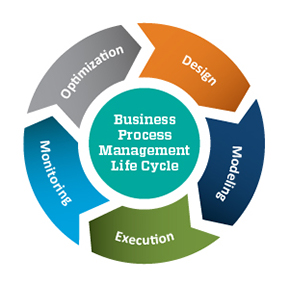
\includegraphics[width=8cm]{./images/BPMN_Lifecycle}
  \captionsource{Lebenszyklus / Phasen von BPMN}{\url{http://legatoconsulting.ca/solutions.html}}
\end{figure}

\begin{itemize}
\itemBfText{Design}{In der Design-Phase werden bestehende und mögliche neue Prozesse identifiziert. Dabei wird der Prozess im Ist-Zustand modelliert.}
\itemBfText{Modelling}{In der Modellierungs-Phase wird der Ist-Prozess analysiert und auf verschiedene Verbesserungsmöglichkeiten hin überprüft.}
\itemBfText{Execution}{In der Execution-Phase wird der verbesserte / veränderte Prozess im Tagesgeschäft umgesetzt. Dies kann, muss aber nicht zwingend, mit Hilfe eines Software-Systems unterstützt oder (teil-) automatisiert werden.}
\itemBfText{Monitoring}{Im Monitoring werden die Prozesse anhand der definierten Metriken und Service Levels gemessen, Statistiken erstellt und mit Benchmarks verglichen.}
\itemBfText{Optimization}{Aufgrund der Informationen aus dem Monitoring und dem Feedback aus dem Tagesgeschäft werden Potenziale für Prozessoptimierungen identifiziert und anschliessend über die Phasen Design, Modelling und Execution umgesetzt.}
\end{itemize}




\subsection{Formalisierung / Notation }
Prozesse können mit Hilfe von Notationen formalisiert und dokumentiert werden. Dazu wird heute entweder die \gls{acr:BPMN} oder die \gls{acr:BPEL} verwendet. Diese beiden Notationen zeichnen sich dadurch aus, dass diese einfach zu erlernen sind und dennoch den Basisregeln von Programmiersprachen folgen. Dadurch wird die Kommunikation zwischen Business und IT erheblich vereinfacht. Ebenfalls können so beschriebene Prozesse relativ einfach in einem System umgesetzt werden.

\subsection{Umsetzung}
\gls{acr:BPM} bietet auf Lange Sicht viele Vorteile für ein Unternehmen. Damit \gls{acr:BPM} in einem Unternehmen erfolgreich ist, ist jedoch eine Veränderung der Unternehmenskultur notwendig. Erst wenn \gls{acr:BPM} teil der Unternehmenskultur ist und aktiv gelebt wird, kann sich das vollständige Potential entfalten.

\subsection{Technische Umsetzung}
Für die technische Umsetzung der in \gls{acr:BPMN} oder \gls{acr:BPEL} definierten Prozesse kann ein \gls{acr:BPMS} eingesetzt werden. Diese Systeme besitzen eine Workflow-Engine, welche in der Lage sind anhand der formalen Prozessdefinition in \gls{acr:BPMN} oder \gls{acr:BPEL} den Prozess abzubilden, beziehungsweise auszuführen und zu (teil-) automatisieren. Typischerweise werden zusätzliche Funktionalitäten zur Definition von Regeln, Interaktionen, Monitoring und Tracking geboten.

\newpage
\subsubsection{Intelligent BPMS}
Die nächste Generation der \gls{acr:BPMS} wird als "`Intelligent \gls{acr:BPMS}"' bezeichnet. Dabei stehen folgende Punkte im Vordergrund:

\begin{itemize}
\item Einblick in die operativen Daten
\item Real-Time Analysen
\item \gls{gls:CEP} (Verarbeitung komplexer Ereignisse)
\item \gls{acr:BMA}
\item Verbesserte Funktionen im Bereich Mobile
\item Verbesserte Funktionen im Bereich Social-Media
\item Verbesserte Funktionen im Bereich Kollaboration
\end{itemize}

% !TeX encoding=utf8
% !TeX spellcheck = de_CH_frami

\chapter{Business Prozesse im Bereich "`Internet of Things"'}

%---------------------------------------------------------------------------------
\section{Die Domäne "`Internet of Things"'}

Bereits fürher: RFID, Sensoren, Machine-Conrols, Messaging Integration, Analytics, Dsahboard -> Kosten und Grösser reduziert

Investitionen in IOT nur sinnvoll, wenn zwischen "`Edge"' uns "`Management"' Software, ist, welche Arbeit vereinfacht / Arbeit übernimmt

\newpage
\subsection{Herausforderungen \& Problemstellungen}

Aktuell: Integration, Impl. Basic Service functions (Lernen von grossen Telekommunikationsfirmen), hoher Effizienzgrad benötigt

\newpage
%---------------------------------------------------------------------------------
\section{Einfluss von \gls{acr:IOT} auf \gls{acr:BPM}}

Wie im Kapitel \ref{sec:Ausg:BPM} beschrieben, hat \gls{acr:BPM} das Ziel eine Vereinfachung herbeizuführen. Da \gls{acr:IOT} einiges an neuer Komplexität mit sich bringt, stellt \gls{acr:BPM} ein geeignetes Mittel dar, um entsprechend einen Teil dieser Komplexität zu reduzieren, beziehungsweise zu abstrahieren.



Evtl. Fragestellung umgekehrt? 
Koordination von Things \& People in der cloud: Erfüllung von Kunden-Needs, Fundamten für IOT: Analyse + Folgeaktion auslösen

	Industrie IOT: nicht IOT, sondern Services bereitstellen, Consumer IOT: mehr auf Geräte fokussiert, anstatt auf Services, BPaas / High volume / on demand / embedded processes -> work with sensors / iot devices -> Eleiminierung repetitiver Prozesse oder Bereitstellung kritischer Prozesse

BPM für Kühlschrank oder Waschmaschine: Kein grosser Benefit wenn nur für Home Use angewendet, interessant im Industrie-Bereich: Just-In-Time-Produktion für Ersatzteile (keine Lager)

BPM: Technology of Work, machine-friendly language of work, abstraktion, schnellere organisation der Arbeit, alternative? Software / code, spezifisch,

Meiste IOT-Projekte: Fokus auf Datensammlung, Analyse - Wenn in Betrieb: Porzesse aus effizienzgründen wichtig - z.B. predictive Mainentane - 10'000, triggers dass Komponente x in den nächsten Tagen ausfallen könnte...was wird mit dieser Datenflut angestellt? -> BPM

Auch negativ: BPM keine Relevanz in IOT: Komplexe Ereignisse und Pattern, konstante Veränderung und Interaktion, Keine Chance in IOT vordefinierte Prozesse einzuhalten, IOT: Komplexe Ereignisverarbeitung und Machine Learning, Kein process mining aufgrund grösser diversität der Daten und konstanten Veränderung, grösste Herausforderung: Privacy

BPM: Zukunft: Input IOT data, Prozesse ermöglichen erst die "`Datengewinnung"' aus den ermittelten Daten

IOT braucht BPMN nicht, umgekehrt, Beziehung nicht symmetrisch, BPM ist mehr spezialisiert, IOT ist "`breiter"'

Gemäss einem Bericht von Gartner (\cite{E:Gartner:BPM:2015}) sollten die Investitionen in \gls{acr:iBPMS} im Jahr 2015 um 4.4\% auf 2.7 Milliarden US-Dollar steigen. Im Rahmen der digitalen Transformation überdenken viele Unternehmen ihre Prozesse und Modelle. Einer der 4 genannten Einflussfaktoren ist \gls{acr:IOT}, wobei die "`Dinge"' in die Business Prozesse integriert werden. Dadurch kann sich der Prozess je nach Bedarf den veränderten Bedingungen anpassen. Durch die gemeinsame Orchestrierung mit allen anderen Prozessteilnehmen können Prozessinovationen einfacher umgesetzt werden.

Nach einem anderen Bericht von Gartner aus dem Jahr 2016 (\cite{E:Gartner:BPM:IOT:2020}) werden im Jahr 2020 mehr als die Hälfte aller neuen Business Prozesse und Systeme in irgendeiner Form ein Element von \gls{acr:IOT} beinhalten.

Stark Abhängig vom Needs der Unternehmen
Input - Entscheid - Reaktion
2 Sichten:
	- Unternehmen (z.B. Industrie) als Enabler, IOT als Kern, Unterstütztend
	- Private 
	
Evtl. aufteilen nach
	- Kern
	- Unterstützend
	- Privat
	

z.B. Predictive maintenance (Beispiel AKW), HealthCare
z.B. Formualr wird von Person ausgefüllt, kann das Formular selbst befüllt werden? (Health Care?) oder Ware wird in Truck verschoben, in Warehouse, Ankunft Kunde
	
Vorteile (Benefits) / Nachteile (Gefahren, etc...) in den Bereichen

Fragestellungen:
-Welche kritischen Prozesse zuerst?
-Wie viel Automatisierung notwenidg / erwünscht
-Wann BPM-Tools, wann Code?


Daten werden analysiert, Reaktionen auf Basis dieser Daten, z.b. Alerts oder korrigierende Schritte, Impact auf kritsche Business Przesse, erfordern integration in operative systeme, 

Effekte: Kosteneinsparungen, Effizienzsteigerungen, mehr revenue patterns, viele herausforderungen für gute umsetzung

Fokus BPMN früher auf: Automatisierung von menschhlichen Aufgaben, streamlining Workflows
IOT spielt eine wichtige Rolle zur Verbesserung der Prozesse in Unternehmen




\newpage
\section{Mögliche Einsatzzwecke von automatisierten Prozessen im Bereich \gls{acr:IOT}}
% z.B. SBB: Stellwerkstörung, Spital

Einsatzmöglichkeiten:
- Lagerhause: Temperatursensor, Threshold erreicht, massnahmen einleiten, wenn nicht erreicht -> benachrichtigung eines menschen

- Auto Versicherung
- Waste Management
- Smart Cities
- Smart Enviornemnts
- Smart Water
- Reatil (Supply Chain control, monitoring storage conditions)
-Industrial Control
-Reduktion Ineffizienten, Energie, Verbesserun glead times, increasing customer services
Beispiel für Prozesse im Bereich IOT
--
Let’s take an example of a fire breaking out at a public parking lot. Someone in the security team would call the building administration who would in turn inform various agencies including fire tenders etc. If someone wants to take stock of the overall status or deliver a coordinated response, it could be days before the information is recorded and reviewed. Look at an alternate reality, the fire sensors in the parking lot detect a fire and immediately cause a fire hazard case to be recorded. This causes immediate email and SMS messages to various agencies including fire tenders and police. The latest pictures and location can be captured by the parking security to make it easier for agencies and administration. The various agencies can provide the latest updates directly via various mobile handhelds. At any point of time, everyone has a clear picture of what’s going on.

A certain flight from London to Dubai gets delayed by 2 hours. Today it would mean 2 frustrating hours of waiting in the lounge or randomly browsing through shops. However IoT could radically change this experience. It could turn into an excellent opportunity for airport retailers and a pleasant couple of hours for passengers. This is how it could work - the information on flight delays is relayed in real time, the retailer then offers a discount sale with details being sent to the passenger mobiles. The Airport Wifi could accurately determine the current location of the passenger (assuming the passenger logs on to the airport app to access free WiFi) and then guide the passengers to the right shop. Based on the passenger profile, the retailer could then offer him a large discount on his favorite brand of cigars.
Today repair and maintenance is one of the most difficult and complex activity in large manufacturing organizations. Consider the advantages of predictive maintenance. When a critical shop floor machine is fitted with sensors, it can know its current condition and wear \& tear and, whenever necessary, initiate its own maintenance process. A combination of sensors and human operators monitor the environment continuously for hazards or damage resulting in reduced risks and maintenance costs.
--



\section{Frameworks, Produkte, ...}
Nachfolgend werden einige Frameworks, beziehungsweise Produkte aufgezeigt, welche im Bereich \gls{acr:IOT} für die Realisierung und Automatisierung von Business Prozessen verwendet werden können.

\begin{itemize}
\itemBfText{IFML}{Plattformunabhängige Beschreibung von UI's, Schwerpunkt auf User-Interaktionen, Interaktions-Optionen, navigations-Pfade, User and System Events, Binding to Business Logic, Binding to Persistance layer, Integration mit BPMN	}
\itemBfText{WSO2}{Middleware, Open Source, Activiti BPM Plattform, Unterstützung: MQTT, OData, Plattform includes: Apache Synapse ESB, Apache Orchestration Director Engine, for operation in DC or cloud, Message Broker suport, trough activiti: BPMN 2.0 support. Details: http://www.infoq.com/news/2015/12/wso2-iot-process-orchestration}
\itemBfText{Pega}{Gartner 2015: Leader in Magic Quadrant for Intelligent Business Process Management Suites}
\itemBfText{Software AG - Digital Business Plattform}{http://www.softwareag.com/corporate/solutions/iot/default.asp}
\itemBfText{OpenIOT}{http://open-platforms.eu/library/openiot-the-open-source-internet-of-things/}
\itemBfText{Oracle Service Bus}
\end{itemize}

%IBM: http://www.cisco.com/c/en/us/solutions/collateral/enterprise/cisco-on-cisco/t-en-07142014-business-process-ioe.html

% Mögiche Fragestellungen welche in Bezug auf BPMN / IOT zuerst gelöst werden müssen / sollen
%http://enterprise-iot.org/book/enterprise-iot/part-ii-igniteiot-methodology/igniteiot-solution-delivery/building-blocks/iot-technology-profiles/4-middleware/process_efficiency_and_automation/
% !TeX encoding=utf8
% !TeX spellcheck = de_CH_frami

\chapter{BPM in der Domäne "`Home Automation"'}

%---------------------------------------------------------------------------------
\section{Die Domäne "`Home Automation"'}
Im Kontext dieser Arbeit bezeichnet "`Home Automation"' den Gesamten Bereich der Heimautomatisierung im Privatbereich. Darunter wird die (Teil-) Automatisierung von Abläufen im Umfeld rund um das Eigenheim und das Privatleben verstanden.

\begin{figure}[H]
  \centering
  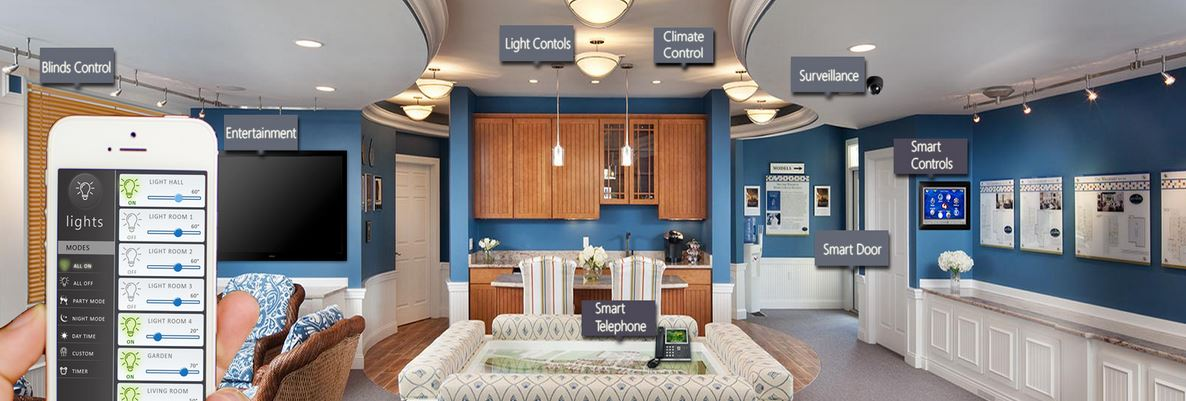
\includegraphics[width=15cm]{./images/home_automation_system}
  \captionsource{Konzeptdarstellung eines "`Smart Home"'}{\url{http://eieihome.com/articles/wp-content/uploads/2015/08/home_automation_system.jpg}}

\end{figure}
"`Home Automation"' oder Heimautomation bezeichnet klassischerweise intelligente die Vernetzung und autonome Kommunikation und Interaktion von Endgeräten in einem "`Eigenheit"'. Das "`Eigenheim"' kann dabei sowohl ein Haus, eine Wohnung oder aber auch ein einzelnes Zimmer oder ähnlich sein. Im Weitesten Sinne gehört auch die Automatisierung von grossen Gebäuden, Gebäudekomplexen oder Siedlungen dazu. Dies wird dann aber meistens unter dem Begriff "`Gebäudeautomation"' zusammengefasst.

Bezogen auf die Anwendung im Eigenheim kommt häufig ein bunter Mix an unterschiedlichen Geräten und Technologien zum Einsatz. Dies stellt eine der zentralen Herausforderungen für die autonome Kommunikation der Geräte dar. Durch den Einsatz einer zentralen Koordinationsstelle (z.B. durch einen Home Automation Hub oder ein Smart Gateway) kann hier Abhilfe geschaffen werden. Diese Koordinationsstellen unterstützen in der Regel eine breite Palette an Übertragungs- und Kommunikationsprotokollen und können so zwischen den verschiedenen Endgeräten vermitteln. 

\subsection{Herausforderungen \& Problemstellungen}
Zusätzlich zu den allgemeinen Herausforderungen und Problemstellungen des \gls{acr:IOT} (Siehe dazu das Kapitel \ref{sec:AnalyseIot:ChallangesAndProblems} \nameref{sec:AnalyseIot:ChallangesAndProblems}) hat der Bereich "`Home Automation"' noch eine Reihe spezifischer Herausforderungen und Problemstellungen, welche es zu bewältigen gibt.

\begin{itemize}
\item Einfache Bedienung
\item Integration mit beliebigen Geräten
\item Fehlende Standards und einheitliche Protokolle
\item Vielfalt an Geräten und proprietären Technologien und Protokollen
\item Flexibilität (Umfeld der Anwendung ist unbekannt)
\item Zentrale Steuerung
\item Sicherheit
\item Stabilität
\item Zuverlässigkeit
\item Gutes Kosten- / Nutzenverhältnis
\item Fachwissen / Technisches Know-How kann nicht vorausgesetzt werden.
\end{itemize}

\subsection{Prognose und Zukunft}
Dem Bereich "`Home Automation"' und insbesondere auch "`Smart Home"' wird ein grosses Wachstumspotenzial für die nächsten Jahre prognostiziert. Gartner zufolge könnte im Jahr 2020 eine durchschnittliche Familie über 500 "`Smart Devices"' besitzen \cite{E:Gartner:Prognose:SmartHome}. Beim grössten Teil dieser Geräte wird es sich um intelligente Haushaltsgeräte handeln. Zu Beginn vorwiegend kleinere Haushaltsgeräte und längerfristig auch zunehmend die grösseren Haushaltsgeräte wie Kühlschränke, Backöfen oder Geschirrspüler. Einer der Schlüssel Aspekte wird gemäss Gartner die Wireless-Technologie sein.

Gemäss Juniper Research werden im Jahr 2020 rund 100 Milliarden US-Dollar für "`Smart Home Services"' (Dienstleistungen und Geräte aus dem Bereich Smart Home) ausgegeben werden. Darin enthalten sind Produkte und Dienstleistungen aus den Bereichen Unterhaltung, Gesundheit, Energie und Heimautomatisierung.

Aufgrund der aktuellen Entwicklung besteht im Bereich "`Smart Home"' und "`Home Automation"' enormes Potenzial für Innovationen und die Erschliessung von neuen Anwendungsmöglichkeiten und Geschäftsfeldern. 

%---------------------------------------------------------------------------------
\section{BPM im Kontext von "`Home Automation"'}\label{sec:Analyse:HA:Kontext}
Der Einsatz von \gls{acr:BPM}, beziehungsweise die dafür verwendeten Notationen \gls{acr:BPMN} und \gls{acr:BPEL}, fokussierte und fokussiert sich nach wie vor primär auf Unternehmen. Aufgrund des notwendigen Know-Hows ist die Verbreitung im Privatumfeld nicht sehr hoch. Entsprechend gibt es nur eine eingeschränkte Auswahl an Frameworks, Lösungen und Produkten, welche explizite Funktionalitäten mit \gls{acr:BPMN} oder \gls{acr:BPEL} beinhalten. Viel mehr werden alternative, beziehungsweise proprietäre Techniken verwendet, um Abläufe zu modellieren. Dabei werden Abläufe zum Beispiel in Form von Auslösern (Triggern) und Aktionen (Actions) modelliert. Je nach Produkt können pro Auslöser auch mehrere Aktionen definiert werden, welche sequentiell abgearbeitet werden.

Der Vorteil dieser Umsetzung ist die tiefe Einstiegshürde und einfache Verständlichkeit und Erlernbarkeit. Gerade im Umfeld der Heimautomation ist es wichtig, dass sich die Verwendung so einfach als möglich gestaltet. Andernfalls werden die Kunden abgeschreckt und setzen lieber auf eine einfacher zu handhabende Lösung.

Der Nachteil des Trigger / Action Ansatzes und damit der Vorteil von \gls{acr:BPMN} und \gls{acr:BPEL} ist die Plattformneutralität und dadurch die Portabilität. Mit diesen Notationen könnten gängige Abläufe einfach und bequem mit anderen Leuten geteilt werden. Auch wäre die Umstellung auf eine andere Lösung aufgrund der Plattformneutralität einfacher zu bewerkstelligen. Dem gegenüber steht der Fakt, dass für \gls{acr:BPMN} und \gls{acr:BPEL} spezifisches Fachwissen benötigt, was entsprechend die Einarbeitungszeit erhöht und dadurch die Einstiegsschwelle anhebt.

Allgemein Betrachtet bietet die Automatisierung und Formalisierung von Abläufen im Home Automation Bereich einige Vorteile. Damit einher gehen aber auch einige signifikante Nachteile.

Das Anwendungsgebiet von Home Automation ist sehr breit gefächert und stark geprägt von den eingesetzten Endgeräten und den genutzten Funktionen. Vor dem Einsatz von \gls{acr:BPMN} und \gls{acr:BPEL} gilt es in jedem Fall die spezifischen Vor- und Nachteile abzuwägen. 



\section{Anwendungsmöglichkeiten}
Für \gls{acr:BPM} oder allgemein die Automatisierung von Abläufen im Bereich des Eigenheimes gibt es eine Reihe von Anwendungsgebieten. Nachfolgend werden einige ausgewählte Szenarien beschrieben:

\begin{itemize}
\itemBfText{Ferienabwesenheit}{Mit einem intelligent vernetzten und automatisierten Eigenheim können viele Tätigkeiten autonom oder via "`Fernbedienung"' durchgeführt werden, für welche andernfalls eine Person Zutritt zur Wohnung haben müsste. Nachfolgend werden einige Beispiel aufgelistet.

\begin{itemize}
\item Giessen von Pflanzen
\item Schliessen der Rollläden am Abend oder bei Sturm
\item Absenkung / Anhebung der Raumtemperatur nach der Abreise / vor der Rückkehr
\item Einbruchsschutz (durch Steuerung von Licht / Ton / Rollläden)
\item Alarmsystem bei einem Notfall
\item Einsparung von Strom (automatische Abschaltung nicht benötigter Geräte)
\item Absicherung, dass alle Fenster geschlossen und Herdplatten ausgeschaltet sind
\end{itemize}}

\itemBfText{Schlechtes Wetter / Sturmm}{Im Haushalt befindet sich eine Wetterstation, welche anhand der gesammelten Messwerte und den Vorhersagen und Informationen von lokalen Wetterdiensten die aktuelle Wetterlage bestimmen kann. Wird festgestellt, dass ein Sturm aufzieht werden automatisch alle Fenster geschlossen, die Rollläden heruntergelassen und die Sonnenstoren eingefahren. Ist niemand Zuhause werden entsprechende Benachrichtigungen an die Bewohner versendet. Beinhaltet die Vorhersage eine Hagelwarnung oder starke Sturmwarnung könnte der Bewohner zusätzlich informiert werden, dass er zum Beispiel sein Auto in die Garage stellen soll, um Schäden zu vermeiden.}

\itemBfText{Türklingel}{Klingelt es an der Tür kann das System aufgrund der verbauten Kamera feststellen, wer sich an der Tür befindet. Handelt es sich um eine bekannte Person, welche erwartet wird, kann die Türe automatisch geöffnet und der Bewohner entsprechend informiert werden. Handelt es sich um eine unbekannte Person, wird der Bewohner benachrichtigt und die Video- und Sprachverbindung zum Aussenbereich hergestellt. Je nach Entscheid des Bewohners wird der Besucher eingelassen oder nicht. Ist der Bewohner nicht zuhause und jemand klingelt an der Tür, wird der Bewohner via Textnachricht informiert und das Foto des Besuchers für eine spätere Überprüfung gespeichert.}
\end{itemize} 


\section{Lösungen, Produkte, Frameworks, ...}\label{sec:Analyse:HA:LPF}
Im Bereich "`Home Automation"' gibt es aktuell viele verschiedene Lösungen, Produkte und Frameworks. Zum einen handelt es sich um reine Softwarelösungen und zum anderen auch um Kombinationen von Hard- und Software. Wie im Kapitel \ref{sec:Analyse:HA:Kontext} \nameref{sec:Analyse:HA:Kontext} erwähnt, gibt es nur wenige Lösungen, welche eine explizite Prozessunterstützung via \gls{acr:BPMN} oder \gls{acr:BPEL} haben.

\subsection{Software Lösungen}
In diesem Abschnitt werden die Software-Lösungen, Produkte und Frameworks aus dem Bereich "`Home Automation"' aufgelistet, welche durch die Recherche ermittelt wurden. Diese wurden jeweils auf rudimentär auf ausgewählte Eigenschaften hin überprüft. Als Quelle für die Zuordnung der Eigenschaften diente der jeweilige Webauftritt und die ersten Einschätzungen aufgrund einer groben Analyse der dazugehörigen Dokumentationen. Eine detaillierte und tiefer führende Analyse der einzelnen Lösungen wurde nicht durchgeführt (Siehe Kapitel \ref{sec:Abgrenzung} \nameref{sec:Abgrenzung}).

Diese Zuordnung dient in erster Linie dazu, einen groben Überblick über die verschiedenen Lösungen zu schaffen und dadurch eine Basis für den weiteren Verlauf der Arbeit zu erhalten.

\begin{longtable}{R{4cm} | c  | c | c | c | c | c | c | c | c | c | c}
	& \THrot{\textbf{Enduser}}
	& \THrot{\textbf{Technisches Know-How notwendig}}
	& \THrot{\textbf{Cloud-basiert}}
	& \THrot{\textbf{Web-basiert}}
	& \THrot{\textbf{Ready-To-Use}}
	& \THrot{\textbf{Framework}}
	& \THrot{\textbf{Trigger \& Action}}
	& \THrot{\textbf{Workflow / Prozesse}}
	& \THrot{\textbf{BPMN / BPEL}}
	& \THrot{\textbf{Open Source / frei verfügbar}}
	& \THrot{\textbf{Lauffähig unter Raspbian 32-Bit}} \\
\midrule
\endhead
\hyperlink{https://ifttt.com/}{IFTTT}  \footnote{\url{https://ifttt.com/https://ifttt.com/}}	
	& 	x
	&	
	&	x		
	& 	x 
	&	x
	&	
	&	x
	&	
	&
	& 	x
	&	\\
\midrule
\hyperlink{https://github.com/foxmask/django-th}{Trigger-Happy (IFTTT Clone)} \footnote{\url{https://github.com/foxmask/django-th}}
	& 	x
	&	(x)
	&			
	& 	x 
	&	x
	&	
	&	x
	&	
	&
	& 	x	
	&	x\\
\midrule
\hyperlink{http://www.theintegratedconnection.com/coco-wireless-home-automation/}{CoCo}  \footnote{\url{http://www.theintegratedconnection.com/coco-wireless-home-automation/}}
	& 	x
	&	
	&	(x)\footnotemark[11]
	& 	(x)\footnotemark[11]
	&	
	&	
	&	x
	&	
	&
	&	
	&	\footnotemark[12] \\
\midrule
\hyperlink{https://home-assistant.io/}{Home Assistant} \footnote{\url{https://home-assistant.io/}}	
	& 	x
	&	(x)	
	&	
	& 	x
	&	x
	&	
	&	x
	&	
	&
	& 	x
	&	x\\
\midrule
\hyperlink{http://www.control4.com/solutions/smart-home-overview}{Control4} \footnote{\url{http://www.control4.com/solutions/smart-home-overview}}	
	&	x
	&	
	&	(x)\footnotemark[11]
	&	\footnotemark[12]
	&
	&
	&	\footnotemark[12]
	&	\footnotemark[12]
	&	\footnotemark[12]
	&	
	&  \footnotemark[12] \\
\midrule
\hyperlink{http://universaal.sintef9013.com/index.php/en/}{universAAL} \footnote{\url{http://universaal.sintef9013.com/index.php/en/}}	
	& 
	&	x
	&	
	&	x
	&	
	&	x
	&	x
	&
	&
	&	x 
	&  \footnotemark[12] \\
\midrule
\hyperlink{http://www.indigodomo.com/}{indigo domotics (Pro Version)} \footnote{\url{http://www.indigodomo.com/}}	
	& 	x
	& 
	&	
	&	x
	&	x
	&	
	&	x
	&	
	&	
	&
	&	\\
\midrule
\hyperlink{http://www.openhab.org/}{openHAB} \footnote{\url{http://www.openhab.org/}}	
	&	x
	&	x
	&	
	&	x
	&	x
	&	
	&	x
	&	(x)\footnotemark[12]
	&	
	&	x 
	&	x\\
\midrule
\hyperlink{http://www.domogik.org/en/}{Domogik} \footnote{\url{http://www.domogik.org/en/}}	
	&	x
	&  (x)
	&
	&	x
	&	x
	&
	&	x
	&
	&
	& 	x 
	&   x\\
\midrule
\hyperlink{http://www.opensourceautomation.com/}{Open Source Automation} \footnote{\url{http://www.opensourceautomation.com/}}	
	&	x
	&	
	&	
	&	x
	&	x
	&	
	&	\footnotemark[12]
	&	\footnotemark[12]
	&
	&	x 
	& \\
\midrule
\hyperlink{http://www.comfortclick.com/}{Comfortclick bOS} \footnote{\url{http://www.comfortclick.com/}}	
	&	x
	&	(x)
	&	
	&	\footnotemark[12]
	&	x
	&	
	&	x
	&	x
	&
	&	x 
	&   (x)\footnotemark[13]\\
\midrule
\hyperlink{http://www.castleos.com/}{CastleOS} \footnote{\url{http://www.castleos.com/}}	
	&	x
	&	
	&	
	&	x
	&	x
	&	
	&	x
	&	
	&		
	&	x
	& 	\\
\midrule 
\hyperlink{http://www.homegenie.it/}{HomeGenie} \footnote{\url{http://www.homegenie.it/}}	
	& x
	& x
	& 
	& x
	& x
	& 
	& x
	& x
	& 
	& x
	& x\\
	
\midrule
\hyperlink{http://www.freedomotic.com/}{Freedomotic} \footnote{\url{http://www.freedomotic.com/}}	
	& x
	& 
	& 
	& x\footnotemark[11]
	& x
	& 
	& x
	& x
	& 
	& x
	& x\\
	
\midrule
\hyperlink{https://netbeast.co/}{Netbeast} \footnote{\url{https://netbeast.co/}}	
	& (x)
	& x
	& 
	& x
	& x
	& x
	& x
	& x
	& 
	& x
	& x \\
	
\midrule
\hyperlink{http://www.domoticz.com/}{Domoticz} \footnote{\url{http://www.domoticz.com/}}	
	& x
	& (x)
	& 
	& x
	& x
	& 
	& \footnotemark[12]
	& \footnotemark[12]
	& 
	& x
	& x\\
\bottomrule
\end{longtable}

\footnotetext[11]{Möglich, aber optional}
\footnotetext[12]{Keine Informationen verfügbar}
\footnotetext[13]{Nur mit kostenpflichtiger Hardware.}

\newpage
Die betrachteten Lösungen sind grundsätzlich alle für den Endbenutzer einsetzbar. Es gibt zudem weitere Angebote im Bereiche Business-2-Business. Dabei werden Unternehmen ganze Plattformen (Hardware und Software) zur Verfügung gestellt, um eigene Home Automation Lösungen zu konzipieren und zu vertreiben (White Label Produkte).

\subsection{Hardware Lösungen (inkl. abgestimmter Software)}
Auf dem Markt gibt es aktuell eine ganze Reihe von kombinierten Lösungen bestehend aus Hard- und Software. Viele davon sind proprietär ausgelegt, sodass diese nur mit Produkten der entsprechenden Produktlinie, den Produkten vom selben Hersteller oder dessen Partnern funktionieren. Darüber hinaus gibt es auch Lösungen, welche einen eher generischen Ansatz verfolgen. Dabei können Produkte von unterschiedlichsten Herstellern angeschlossen werden. Voraussetzung ist jeweils, dass das entsprechende Protokoll und die Funktionalitäten unterstützt werden.

Nachfolgend werden einige der recherchierten Lösungen aufgelistet. Diese werden jedoch im Rahmen dieser Arbeit nicht weiter analysiert.

\begin{itemize}
\item Bosch G100 Z-Wave Home Control Gateway
\item Samsung Smart things
\item Qivicon
\item Zoo Automation
\item Throne BMS
\end{itemize}

\subsection{Weitere}
Neben Software basierten und Kombinationen von Hard- und Software Lösungen gibt es auch Bestrebungen Referenz-Architekturen zu schaffen. Eine davon ist zum Beispiel die  \hyperlink{http://www.ubicomp.org/ubicomp2013/adjunct/adjunct/p801.pdf}{Home Blox}  \footnote{\url{http://www.ubicomp.org/ubicomp2013/adjunct/adjunct/p801.pdf}} Architektur.



% !TeX encoding=utf8
% !TeX spellcheck = de_CH_frami

\chapter{BPM auf dem "`Raspberry Pi"' in der Domäne "`Home Automation"'}
In diesem Kapitel wird analysiert wie Business Prozesse auf einem Raspberry Pi implementiert, beziehungsweise automatisiert werden können. Dabei werden verschiedene Lösungskategorien aufgezeigt und erläutert.


\section{Der Raspberry Pi}
\begin{figure}
  \centering
  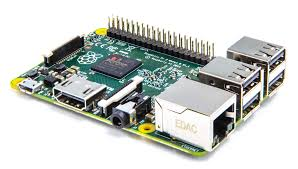
\includegraphics[width=8cm]{./images/RaspberryPi2ModelB}
  \captionsource{Raspberry Pi 2 Model B}{\url{https://www.raspberrypi.org/wp-content/uploads/2015/01/Pi2ModB1GB_-comp.jpeg}}
\end{figure}
  
Der Raspberry Pi ist ein Einplatinencomputer, welcher von der Raspberry Pi Foundation entwickelt und vertrieben wird. Er hat ungefähr die Grösse einer Kreditkarte und bietet zahlreiche On-Board Schnittstellen wie USB-, HDMI und Audio Anschlüsse (Abhängig vom konkreten Modell). Zusätzlich stehen eine bestimmte Anzahl an GPIO-Pins (General Purpose Input / Output) zur Verfügung. Mit Hilfe dieser Pins lassen sich zum einen Erweiterungs-Boards anschliessen und zum anderen können auch eigene Schaltungen, etc. gebaut und verlötet werden. Die Anzahl und genaue Funktion der einzelnen GPIO-Pins ist vom konkreten Raspberry Pi Modell abhängig.

\begin{figure}[H]
  \centering
  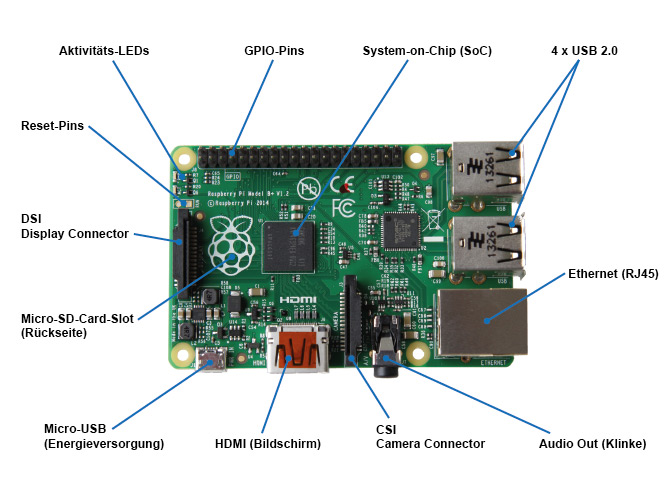
\includegraphics[width=13cm]{./images/RaspberryPi2ModelBPlusOverview}
  \captionsource{Raspberry Pi 2 Model B Überblick}{\url{https://www.elektronik-kompendium.de/sites/raspberry-pi/bilder/19052512.jpg}}
\end{figure}

\newpage
\begin{landscape}

\subsection{Raspberry Pi Modelle im Überblick}
\begin{table}[H]
\centering
\begin{tabular}{r | c  | c | c | c | c | c | c | c | c | c}
	& \THrot{\textbf{Raspberry Pi Model A}}
	& \THrot{\textbf{Raspberry Pi Model A+}}
	& \THrot{\textbf{Raspberry Pi Model B}}
	& \THrot{\textbf{Raspberry Pi Model B+}}
	& \THrot{\textbf{Raspberry Pi 2 Model B}}
	& \THrot{\textbf{Raspberry Pi 3 Model B}}
	& \THrot{\textbf{Raspberry Pi Compute}}
	& \THrot{\textbf{Raspberry Pi Zero}}\\
\midrule
Gewicht in Gramm
	& 	31
	&	23
	&	40		
	& 	45 
	&	40
	&	40
	&	7
	&	9\\
\midrule
System-on-a-Chip (SoC):
	& 	\multicolumn{4}{|c|}{BCM2835} 
	&	BCM2836
	&	BCM2837
	&	\multicolumn{2}{|c|}{BCM2835} \\
\midrule
CPU Kerne
	& 	1
	&	1
	&	1		
	& 	1 
	&	1
	&	4
	&	1
	&	1\\
\midrule
CPU Takt in MHz
	& 	\multicolumn{4}{|c|}{700} 
	&	900
	&	1200
	&	700
	&	1000\\
\midrule
CPU Architektur
	& 	\multicolumn{4}{|c|}{ARMv6 (32-bit)}  
	&	ARMv7 (32-bit)	
	&	ARMv7 (64-bit)	
	&	\multicolumn{2}{|c|}{ARMv6 (32-bit)}  	\\
\midrule
GPU Takt in MHz
	& 	\multicolumn{5}{|c|}{250} 
	&	300/400
	&	\multicolumn{2}{|c|}{250} \\
\midrule
Arbeitsspeicher in MB
	& 	\multicolumn{2}{|c|}{256}  
	&	256 / 512		
	& 	\multicolumn{2}{|c|}{512}  	
	& 	1024 
	&	\multicolumn{2}{|c|}{512}  	\\
	
\midrule
Pins
	& 	26
	&	40
	& 	26
	& 	\multicolumn{3}{|c|}{40}  	
	&	60
	&	40  	\\
	
\midrule
GPIO-Pins
	& 	17	
	&	26
	& 	17
	& 	\multicolumn{3}{|c|}{26}  	
	&	48
	&	26  	\\
\bottomrule
\end{tabular}
\end{table}

%Evtl.: http://praxistipps.chip.de/welcher-raspberry-pi-alle-modelle-im-vergleich_41923

\end{landscape}
\newpage

\section{Betrachteter Lösungsraum}
Ursprünglich wären folgende Einschränkungen für den Lösungsraum vorgesehen gewesen:
\blockquote {Da der Raspberry Pi eine offene Plattform ist, gibt es unterschiedlichste Möglichkeiten um das betrachtete Problem zu lösen. Im Kontext dieser Seminararbeit erfolgt die Betrachtung spezifisch für ein Raspberry Pi 2 Model B mit einem Raspbian OS (Debian Derivat für den Raspberry Pi). Als zusätzliche Prämisse gilt ebenfalls, dass der Kern der Anwendung auf dem Raspberry Pi lauffähig sein muss und die Lösung es in irgendeiner Form ermöglichen muss einen Ablauf / Prozess im Bereich Home Automation mit \gls{acr:BPMN} oder \gls{acr:BPEL} abzubilden. Lösungen, bei denen der Raspberry Pi als "`Client"' / "`Agent"' werden nicht berücksichtigt, da der Raspberry Pi im Fokus steht.}

Die ersten intensiven Recherchen haben gezeigt, dass es keine bis sehr wenige Lösungen gibt, welche diesen Anforderungen erfüllen würden. Daher wurde der Lösungsraum so angepasst , dass zwei unterschiedliche Lösungskategorien geschaffen werden. Eine mehr mit dem Fokus Home Automation und die andere mit Schwerpunkt im Bereich \gls{acr:BPM}.

\textbf{Spezifische Home Automation Lösungen}
\begin{itemize}
\item Lauffähig auf dem Raspberry Pi mit Raspbian (32-Bit)
\item Eine einzige Komponente (Keine Kombination von Komponenten)
\item Open Source / Frei verfügbar (allenfalls Demoversion)
\item Bedienbar via Web
\item Fokus: Home-Automation
\item Funktionalität um Abläufe oder Aktionen zu automatisieren
\end{itemize}

\textbf{Lösung mit \gls{acr:BPMN}-Support im Bereich \gls{acr:IOT}}
\begin{itemize}
\item Lauffähig auf dem Raspberry Pi mit Raspbian (32-Bit).
\item Eine einzige Komponente (Keine Kombination von Komponenten)
\item Open Source / Frei verfügbar (allenfalls Demoversion)
\item Bedienbar via Web
\item Abläufe / Prozesse können mit Hilfe von \gls{acr:BPMN} modelliert werden.
\item Möglichkeit zur Anbindung von \gls{acr:IOT}-Geräten aus dem Bereich "`Home Automation"' (z.B. via Plugins oder Custom-Code).
\end{itemize}


\section{Lösungen, Produkte \& Frameworks }
In diesem Abschnitt werden die recherchierten Lösungen, Produkte und Frameworks aufgezeigt. Diese Aufzählung ist nicht abschliessend und repräsentieren den Stand der Dinge zum Zeitpunkt der Recherchen im Q2/2016.

\subsection{Lösungskategorie: Spezifische Home Automation Lösungen}
Die Inhalte dieser Lösungskategorie wurden aus dem Kapitel \ref{sec:Analyse:HA:LPF} \nameref{sec:Analyse:HA:LPF} entnommen und nach folgenden Kriterien gefiltert:

\textbf{Filterkriterien}
\begin{itemize}
\item Web-basiert
\item Ready-To-Use
\item Kein Framework
\item Trigger \& Action oder Workflow  / Prozess oder BPMN / BPEL Unterstützung
\item Open Source / frei verfügbar
\item Lauffähig unter Raspbian 32-Bit
\end{itemize}

\textbf{Lösungsraum (gefiltert nach Filterkriterien)}
\begin{itemize}
\item TriggerHappy
\item HomeAssistant
\item openHAB
\item Domogik
\item HomeGenie
\item Freedomotic
\item Domoticz
\end{itemize}

Aufgrund eines kurzen Antestens und des daraus resultierenden Eindruckes wurde \textbf{"`openHAB"'} für die Realisierung des Demo-Setups ausgewählt. Die Auswahl erfolgte nicht aufgrund bestimmter Kriterien. Der genaue Setup wird im Abschnitt \ref{sec:AnalyseRPI:Beispiel} \nameref{sec:AnalyseRPI:Beispiel} beschrieben. Das Fazit zur ausgewählten Lösung wird im Kapitel \ref{subsec:Fazit:BPMN:RPI:HA} \nameref{subsec:Fazit:BPMN:RPI:HA} erläutert.


\subsection{Lösung mit BPMN-Support im Bereich IOT}
Der definierte Lösungsraum dieser Lösungskategorie ermöglicht ein breites Spektrum an Lösungen. Nachfolgend werden einige der möglichen Lösungen aufgezeigt. Bei der Auswahl wurden folgende Kriterien berücksichtigt:

\textbf{Filterkriterien}
\begin{itemize}
\item Web-basiert
\item Ready-To-Use
\item Kein Framework
\item Integrierte \gls{acr:BPMN}-Engine
\item Open Source / frei verfügbar
\item Lauffähig unter Raspbian 32-Bit
\end{itemize}

\textbf{Lösungsraum (gefiltert nach Filterkriterien)}
\begin{itemize}
\item \hyperlink{http://activiti.org/}{activiti BPM Platform} \footnote{\url{http://activiti.org/}}
\item \hyperlink{http://www.jbpm.org/}{jBPM} \footnote{\url{http://www.jbpm.org/}}
\item \hyperlink{https://camunda.com/}{Camunda BPM Platform (Community Edition)} \footnote{\url{https://camunda.com/}}
\item \hyperlink{http://www.imixs.org/}{Imixs Workflow} \footnote{\url{http://www.imixs.org/}}
\end{itemize}

Aufgrund des ersten Eindruckes, der eingeschätzten Komplexität und des eingeschätzten Zeitaufwands für die Realisierung eines Beispiel-Setups wurde die \textbf{"`activiti BPM Plattform"'} ausgewählt. Die Einschätzung erfolgte aufgrund der Informationen auf den entsprechenden Produkt-Webseiten und den dazugehörigen Dokumentationen und Beispielen.


%------------------------------------------------------------------
\newpage
\section{Realisierung eines Beispielhaften Prozesses mit BPMN im Bereich "`Home Automation"'} \label{sec:AnalyseRPI:Beispiel}
Nachfolgend wird der realisierte Beispielprozess und die dafür benötigten Komponenten beschrieben.

\subsection{Verwendete Hardware}
Für die Realisierung des Beispiel-Setups wurden folgende Hardware-Komponenten verwendet:
\begin{itemize}
\item \textbf{Raspberry Pi 2 Model B}
\itemBfText{Razberry Board}{Das Razberry Board ist ein Raspberry Pi Erweiterungsboard, welches die Einbindung des Raspberry Pi's in ein Z-Wave Netzwerk ermöglicht. Dabei kann das Razberry Board als Z-Wave Controller verwendet werden.}
\itemBfText{Z-Wave.Me Double Wall Switch}{Z-Wave Wand-Schalter, welcher mit verschiedenen Funktionen programmiert werden kann.}
\itemBfText{domitech Z-Wave Smart LED Light Bulb}{LED Glühbirne, welche über Z-Wave gesteuert werden kann.}
\itemBfText{Ralink Technology, Corp. RT5370 Wireless Adapter}{USB WLAN Adapter}
\end{itemize}

\subsection{Verwendete Software} \label{sec:AnalyseRPI:Beispiel:SW}
Für die Realisierung des Beispiel-Setups wurden folgende Software-Komponenten verwendet.

\begin{itemize}
\itemBfText{NOOBS}{\gls{acr:NOOBS} ist ein Hilfsprogramm zur Installation von Betriebssystemen auf dem Raspberry Pi (Installations-Manager).}

\itemBfText{Raspbian Jessie}{Als Betriebssystem wurde die aktuelle Version von Raspbian Jessie (Debian Derivat).}

\itemBfText{openHAB 2}{Als Schlüsselkomponente wurde openHAB 2 eingesetzt. openHAB 2 ist eine Open Source Lösung für die Heimautomatisierung. Die Basis von openHAB 2 bildet das Eclipse SmartHome Framework der Eclipse Foundation. Die Installation und Konfiguration erfolgte gemäss den Anleitungen und Beispielen im \hyperlink{https://github.com/openhab/openhab/wiki}{GitHub-Wiki von openHAB} \footnote{\url{https://github.com/openhab/openhab/wiki}}.}

\itemBfText{Apache Derby}{Apache Derby ist eine in Java implementierte relationale Datenbank, welche unter der Open Source Apache Lizenz Version 2.0 verfügbar ist. Die Apache Derby Datenbank wurde verwendet um die Persistenz in openHAB zu realisieren. Die Integration erfolgte über das \gls{acr:JPA} Binding von openHAB. Die Apache Derby Installation wurde gemäss der von Apache zur Verfügung gestellten \hyperlink{https://db.apache.org/derby/papers/DerbyTut/install_software.html}{Anleitung}\footnote{\url{https://db.apache.org/derby/papers/DerbyTut/install_software.html}} installiert und konfiguriert. Die Anbindung an openHAB erfolgte gemäss der Dokumentation im \hyperlink{https://github.com/openhab/openhab/wiki/JPA-Persistence}{Wiki} \footnote{\url{https://github.com/openhab/openhab/wiki/JPA-Persistence}}.}

\itemBfText{ejabberd XMPP-Server}{Als \gls{acr:XMPP} Server wurde ejabberd verwendet. \gls{acr:XMPP} Server werden unter anderem für Instant Messaging (Dienst für Sofortnachrichten) eingesetzt. In diesem Setup wurde der \gls{acr:XMPP} Server für die Kommunikation zwischen dem openHAB Server und dem Anwender verwendet. Einerseits kann openHAB über ein Binding Nachrichten an den Anwender senden und andererseits kann der Anwender bestimmte Befehle und Anweisungen an openHAB übermitteln. Die Installation von ejabberd erfolgt anhand der Anleitungen von \hyperlink{https://www.digitalocean.com/community/tutorials/how-to-install-ejabberd-xmpp-server-on-ubuntu}{Digitalocean}\footnote{\url{https://www.digitalocean.com/community/tutorials/how-to-install-ejabberd-xmpp-server-on-ubuntu}} und \hyperlink{https://box.matto.nl/ejabberdjessie.html}{box.matto.nl}\footnote{\url{https://box.matto.nl/ejabberdjessie.html}}. Das openHAB Binding wurde gemäss der Dokumentationen im openHAB-Wik eingerichtet (\hyperlink{https://github.com/openhab/openhab/wiki/Actions\#xmpp-actions}{Action-Bindings}\footnote{\url{https://github.com/openhab/openhab/wiki/Actions\#xmpp-actions}}, \hyperlink{https://github.com/openhab/openhab/wiki/Feature-Overview}{UI's}\footnote{\url{https://github.com/openhab/openhab/wiki/Feature-Overview}}).}

\itemBfText{Mosquitto MQTT Broker}{Mosquitto ist ein Open Source \gls{acr:MQTT} Broker der Eclipse Foundation. \gls{acr:MQTT} ist ein leichtgewichtiges "`Publish-Subscribe"' Protokoll auf Basis von TCP/IP. Innerhalb von openHAB kann \gls{acr:MQTT} unter anderem für die Publikation des aktuellen Status der Geräte / Komponenten verwendet werden. Ebenfalls können Statusänderungen für Geräte / Komponenten über den \gls{acr:MQTT} Server ausgeführt werden. Mosquitto wurde gemäss der Anleitung von \hyperlink{https://www.digitalocean.com/community/questions/how-to-setup-a-mosquitto-mqtt-server-and-receive-data-from-owntracks}{Digitalocean}\footnote{\url{https://www.digitalocean.com/community/questions/how-to-setup-a-mosquitto-mqtt-server-and-receive-data-from-owntracks}} installiert. Die Konfiguration in openHAB erfolgte gemäss der Anleitung im \hyperlink{https://github.com/openhab/openhab/wiki/MQTT-Binding}{Wiki}\footnote{\url{https://github.com/openhab/openhab/wiki/MQTT-Binding}}.}

\itemBfText{openHAB Bindings}{Neben den beschriebenen Komponenten wurden diverse weitere Bindings und Actions innerhalb von openHAB verwendet.}

\itemBfText{Apache Tomcat 7}{Um die BPM Plattform "`activiti"' zu nutzen wurde der Open Source Web Server Apache Tomcat 7 eingesetzt. Die Installation erfolgte gemäss der Anleitung von \hyperlink{https://www.digitalocean.com/community/tutorials/how-to-install-apache-tomcat-7-on-ubuntu-14-04-via-apt-get}{Digitalocean}}\footnote{\url{https://www.digitalocean.com/community/tutorials/how-to-install-apache-tomcat-7-on-ubuntu-14-04-via-apt-get}}.

\itemBfText{activiti BPM Plattform}{Activiti ist eine Java-basierte Open Source Workflow und \gls{acr:BPM} Plattform. Die Beispielsapplikation wurde gemäss den Informationen im \hyperlink{http://activiti.org/userguide/index.html}{User-Guide}\footnote{\url{http://activiti.org/userguide/index.html}} und den Beispiels-Anwendungen "`activiti-explorer"' und "`activiti-rest"' implementiert. }

\itemBfText{H2}{Die H2 Datenbank ist eine Open Source Java SQL Datenbank, welche als Backend der activiti BPM Plattform eingesetz wird. Die Installation erfolgte gemäss der Anleitung von \hyperlink{http://www.h2database.com/html/tutorial.html}{H2}\footnote{\url{http://www.h2database.com/html/tutorial.html}}.}

\itemBfText{Postfix}{Der Postfix-Mail-Server wurde zum Versand von lokalen E-Mail's verwendet. Dieser Mail-Server wird von der activiti BPM Plattform verwendet, um Benachrichtigungen innerhalb des Prozesses zu versenden. Die Installation und Konfiguration erfolgte gemäss der Anleitung von \hyperlink{https://www.digitalocean.com/community/tutorials/how-to-install-and-setup-postfix-on-ubuntu-14-04}{Digitalocean}\footnote{\url{https://www.digitalocean.com/community/tutorials/how-to-install-and-setup-postfix-on-ubuntu-14-04}}.}

\itemBfText{Pidgin Internet Messenger}{Auf der Client-Seite wurde für die Kommunikation mit ejabberd der "`Pidgin Internet Messenger"' verwendet.}

\itemBfText{Linux Utilities und Tools}{Es wurden diverse weitere Linus-Utilites und Tools für die Implementation und die Arbeit mit den Komponenten verwendet (unter anderem: screen, scp, Eclipse IDE).}
\end{itemize}


\subsection{Komponentenübersicht}
Die Abbildung \ref{img:AnalyseRpi:ComponentOverview} \nameref{img:AnalyseRpi:ComponentOverview} zeigt die im Kapitel \ref{sec:AnalyseRPI:Beispiel:SW} \nameref{sec:AnalyseRPI:Beispiel:SW} beschriebenen Komponenten grafisch auf und zeigt deren direkten Abhängigkeiten auf. Sämtliche Komponenten wurden befinden sich auf dem Raspberry Pi. Der Grossteil der Komponenten muss nach dem Start durch ein Shell-Script gestartet werden.

\begin{landscape}
\begin{figure}[H]
  \centering
  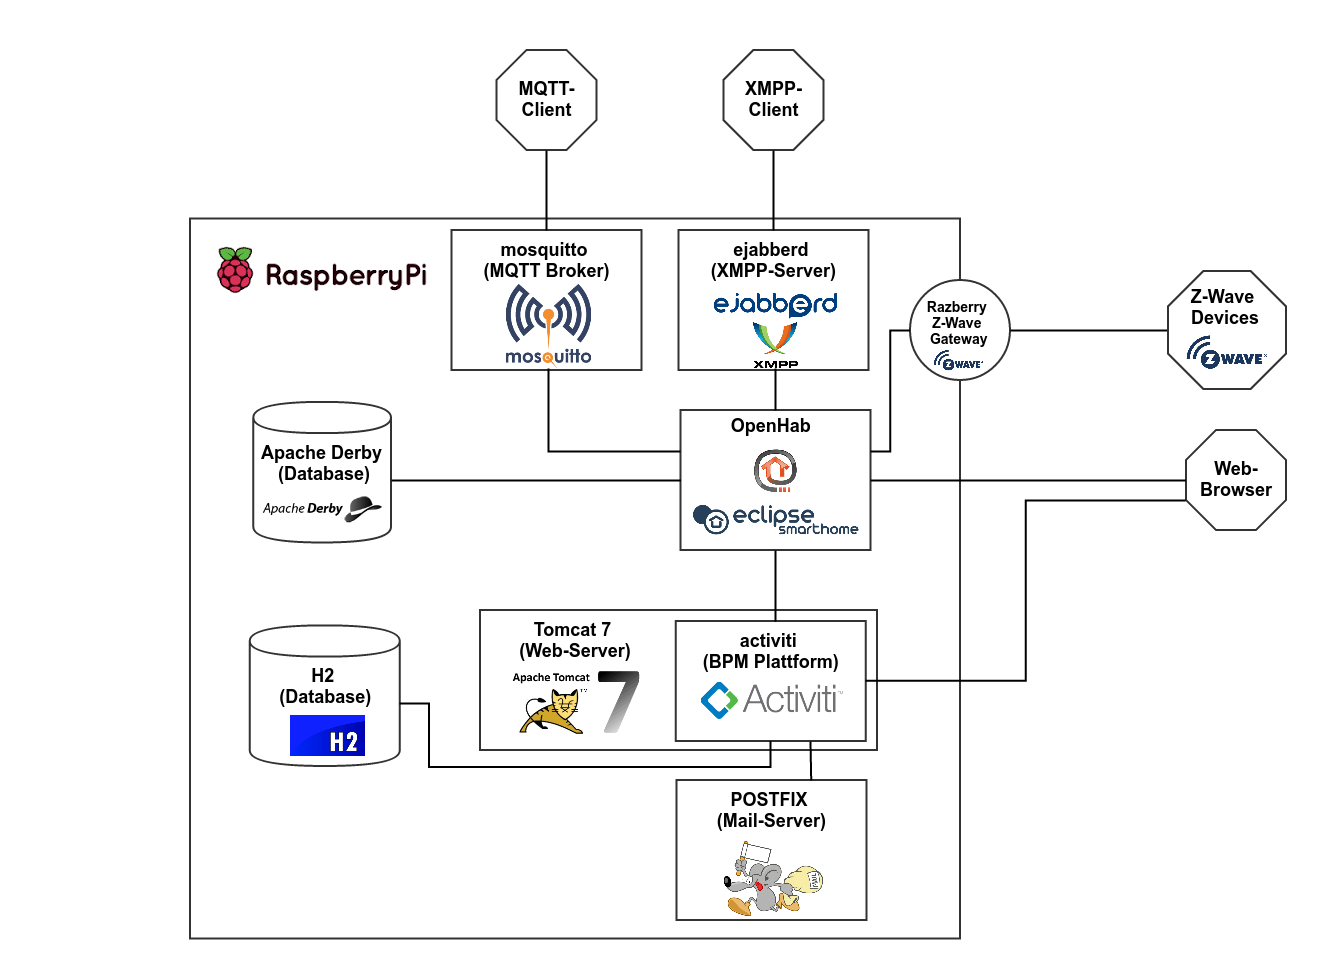
\includegraphics[width=19cm]{./images/Component-Overview}
  \caption{Komponentenübersicht}\label{img:AnalyseRpi:ComponentOverview}
\end{figure}
\end{landscape}

\subsection{Prozess / Szenario}
Als Beispiel wurde der Prozess "`Türklingel"' beschrieben und umgesetzt. Formal wurde der Prozess gemäss der \gls{acr:BPMN} 2.0 Spezifikation beschrieben. Der formale Prozess ist in der Abbildung \ref{img:AnalyseRpi:DoorbellProcess} \nameref{img:AnalyseRpi:DoorbellProcess} ersichtlich.

Bei der Umsetzung des konkreten Beispiels wurden nicht alle Komponenten verwendet, welche im Kapitel \ref{sec:AnalyseRPI:Beispiel:SW} \nameref{sec:AnalyseRPI:Beispiel:SW} beschrieben wurden (zum Beispiel: MQTT-Broker und Persistent von OpenHab).

{\small \textbf{Hinweis: }}
\subsubsection{Beschreibung}
Der "`Türklingel"' Prozess definiert das Verhalten des "`Smart-Home"' wenn jemand an der Türe klingelt. Dabei werden bestimmte Kriterien geprüft, um den zu durchlaufenden Prozesszweig zu evaluieren.

\subsubsection{Ausbau- und Verbesserungsmöglichkeiten}

\subsubsection{Start-Event}
Der Start des Prozesses erfolgt in der gewählten Home Automation Lösung (openHAB 2). In openHAB wurde ein Z-Wave Wandschalter eingerichtet. Für diesen Wandschalter wurde eine Regel definiert, welche bei einer Statusänderung ausgeführt wird. 

\begin{lstlisting}
Code goes here
\end{lstlisting}

\subsubsection{Abrufen der Status-Informationen}

\subsubsection{Auswerten der Status-Informationen}

\subsubsection{Verzweigung: "`User ist zu Hause"'}

\subsubsection{Verzweigung: "`User ist nicht zu Hause"'}

\subsubsection{Verzweigung: "`User ist in den Ferien"'}
\todo{Beschreibung}

\newpage
\begin{landscape}
\begin{figure}[H]
  \centering
  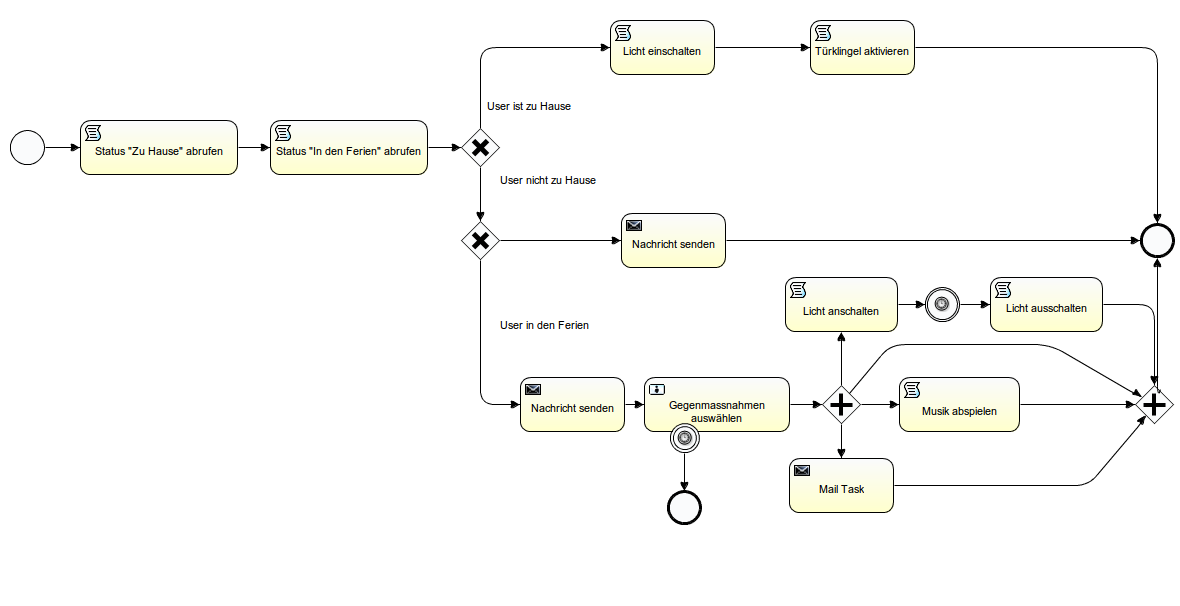
\includegraphics[width=21cm]{./images/DoorBellProcess}
  \caption{"'Türklingel-Prozess"'}\label{img:AnalyseRpi:DoorbellProcess}
\end{figure}
\end{landscape}

% !TeX encoding=utf8
% !TeX spellcheck = de_CH_frami

\chapter{Schlusswort} \label{chap:Finish}

%---------------------------------------------------------
\section{Fazit}

\subsection{Internet of Things}
\subsection{Home Automation}
Im Bereich "`Home Automation"' gibt es gemäss heutigem Stand nur ...

Die meisten Softwarelösungen und Kombi-Produkte (Software + Hardware) basieren auf dem Konzept von Auslösern (Triggern) und nachfolgenden Ereignissen (Events).

Heimanwender: BPM Schwierig, wenn dann im Bereich der Gebäude-Automatisierung im Bereich von Unternehmen.


OPENHAB:
Version 1: Schwieriger / Komplizierter Setup (insbesondere mit Z-Wave)

Version 2: Einfacherer Setup, viele fehlende Funktionalitäten, nicht intutitiv, Dokumentation für gewisse Grundkonzepte nicht wirklich gut

\subsection{Home Automation + Raspberry Pi}
Evtl. Getrennte Fazite für einzelne Bereiche?


\subsection{Allgemein}
Aufgrund der Ergebnisse der Analyse kann gesagt werden, dass aktuell im Bereich der Modellierung und Implementierung von Business Prozessen ein Wandel statt findet. Mit diesem Wandel rückt der Einsatz des \gls{acr:IOT} etwas mehr in den Vordergrund. 

....Bereits erste Produkte / Lösungen mit entsprechendem Support.



%---------------------------------------------------------




%---------------------------------------------------------

\section{Dank}


% --- Moved Glossary ---
\IfPackagesLoaded{glossaries,longtable,tabu}{
  \cleardoublepage
  % print out acronym list   
  \IfGlossariesStyleDefined{longtabuFancyHeader}
   {\printglossary[type=\acronymtype,style=longtabuFancyHeader]}
  % print out symbol list 
  \IfGlossariesStyleDefined{longtabuFancyHeader}
   {\printglossary[type=symbolslist,style=longtabuFancyHeader]}
  % print out glossary
  \printglossary[style=altlist]
} % end of glossaries

%%% -- end of main content

% -- bibliography --
% (must be placed _before_ appendix)

% show all biblatex entries
\nocite{*}

% set title
\renewcommand\bibname{Quellenverzeichnis}

\IfPackageLoaded{biblatex}{
  \cleardoublepage
  \IfDefined{phantomsection}{\phantomsection}\label{sec:bibliography}
  \printbibliography[%
    heading=bibintoc, % (bibintoc, bibnumbered)
  ]	
}% end of bibliography

%% -- list of figures and tables --
\cleardoublepage\IfDefined{phantomsection}{\phantomsection}\label{sec:lof}
\listoffigures
%\cleardoublepage\IfDefined{phantomsection}{\phantomsection}\label{sec:lot}
%\listoftables

%% -- List of Listings --
% _Remove_ if no listing with caption is defined
% \IfDefined{lstlistoflistings}{\cleardoublepage\lstlistoflistings}

% --- Appendix --- --- --- --- --- --- ---

\cleardoublepage
\appendix
% Add `Appendix` to TOC
\addcontentsline{toc}{part}{\appendixname}
%% must be _input_, otherwise the TOC entry is at the wrong place
% % !TeX encoding=utf8
% !TeX spellcheck = de_CH_frami

%
% add files for appendix chapter here

%\input{content/Z-App-Survey.tex} \label{appendix:Survey}

%\input{content/Z-App-SurveyResults.tex} \label{appendix:SurveyResults}

\chapter{Vorlage: Protokoll}


Tabelle mit : Laufnummer, Zeit, Befehl / Aktion, Hash Ergebnisdatei, Kommentar


\chapter{Vorlage: Beweiszettel}
Buch CF: Seite 85

Beweiskette:

Laufwerke: Manufacturer, Model, Serial Number, Evidence Description (Name of suspect, Technologie: SATA, IDE, ...)


\chapter{Vorlage: Formular Incident-Meldung}
-Richtige Informationen abfragen (Merkblatt / Chekliste)
--Basisinfos: Aktuelle Uhrzeit, Wer / Welches System berichtet Vorfall, Art und Weise Vorfall, Vermuteter Zeitpunkt Vorfall, mittelbar / unmittelbar betroffene HW / SW, evtl. Auswirkungen, Schaden, Kontakstelle für ISR und Ermittler
--Infos über betroffenes System sammeln (!! möglichst nicht vom System abfragen, Datenklassifizierung? Klassifizierung? Ort?, Physischer Zugang?  allgemeiner Systemzustand,)
--Angreifer: Infos? noch aktiv? Systeme / Daten manipuliert / zerstört, Vermutungen?
--Getroffene Massnahmen / System verändert? Andere Perosnen benachrichtigt?


\chapter{Ablauf einer forensischen Analyse}


% -- only in phd thesis --->
%% !TeX encoding=utf8
% !TeX spellcheck = de_CH_frami

%% This list is from the phd publication 
%% of Matthias Pospiech
%% 
\chapter*{Publications}
\markboth{Publications}{Publications}

\IfPackageLoaded{hyperref}{
	\phantomsection
	\addcontentsline{toc}{chapter}{Publications}
}

%% In these lists the publications are numbered by date of publications
%% and the author of the thesis can be printed in bold.

\section*{Scientific publications}
% \section*{Wissenschaftliche Veröffentlichungen}
\begin{refsection}
\nocite{Siegel2007, Palmer2010, Pospiech2009, Pospiech2010, Pospiech2011}
% print all combinations in this list bold (makes name of author bold)
\forcsvlist{\listadd\bibboldnames}
  {{Pospiech, Matthias}, {Pospiech, M.}}
\printbibliography[env=numbered+bold, heading=none, sorting=ynt, resetnumbers=true]
\end{refsection}

\section*{Submissions to international conferences}
% \section*{Beiträge auf internationalen Konferenzen}
\begin{refsection}
\nocite{Morgner2008, Palmer2008a, Siegel2008,Pospiech2009a,Pospiech2010b,Pospiech2010a}
% print all combinations in this list bold (makes name of author bold)
\forcsvlist{\listadd\bibboldnames}
  {{Pospiech, Matthias}, {Pospiech, M.}}
\printbibliography[env=numbered+bold, heading=none, sorting=ynt, resetnumbers=true]
\end{refsection}

\section*{Submissions to national conferences}
% \section*{Beiträge auf nationalen Konferenzen}
\begin{refsection}
\nocite{EmonsDPG2009, HoffmannDPG2008, LangDPG2008, VaeckenstedtDPG2010, PospiechDPG2009, PospiechDPG2010, PospiechDPG2011}
% print all combinations in this list bold (makes name of author bold)
\forcsvlist{\listadd\bibboldnames}
  {{Pospiech, Matthias}, {Pospiech, M.}}
\printbibliography[env=numbered+bold, heading=none, sorting=ynt, resetnumbers=true]
\end{refsection}
%
% standard style
\renewcommand*{\bibboldnames}{}

%% !TeX encoding=utf8
% !TeX spellcheck = de_CH_frami

\chapter*{Curriculum Vitae}
\markboth{Curriculum Vitae}{Curriculum Vitae}

\IfPackageLoaded{hyperref}{
	\phantomsection
	\addcontentsline{toc}{chapter}{Curriculum Vitae}
}

\IfPackagesLoaded{currvita,csquotes}{%

%% - notes --------------------
\minisec{Delete these notes:}
\small
This is a modified version of a german CV.
I have not translated it into English, because
I am not familiar with English CV styles.

Remember that you do not write this CV to apply for a job.
This is just a brief summary of your previous research career.
A `real' CV is much more complex!
\normalsize
%% -----------------------------

\begin{cv}{}
\begin{cvlist}{Personalien}
	\item[Name]
		Max Musterman \\
		geboren am 01.02.1979 in Berlin \\
		ledig, deutsch
\end{cvlist}
%
\begin{cvlist}{Schulbildung}
	\item[1998] Abitur, Gymnasium Musterschule in Berlin
\end{cvlist}
%
\begin{cvlist}{Zivildienst}
	\item[07/98 - 08/99] 
	<Einfügen>
\end{cvlist}
%
\begin{cvlist}{Studium}
	\item[SS/99 - SS/06] Universität Hannover, Studium der Physik
	\\[0.5\baselineskip]
Thema der Diplomarbeit: \enquote{Charakterisierung des Rauschverhaltens eines 
weit abstimmbaren Ytterbium dotierten kerngepumpten Faserlasers}, durchgeführt 
am Laserzentrum Hannover e.\,V.
	\item[Mai 2006] Abschluss: Diplom-Physiker	
\end{cvlist}
%
\begin{cvlist}{Promotion}
	\item[09/2006 - heute] Wissenschaftlicher Mitarbeiter am Institut für 
Quantenoptik, Leibniz Universität Hannover
\end{cvlist}

\end{cv}

}{}%
% <------------------------

%% -- Index --
% _Remove_ Index unless you really want to invest a large amount
% of time and effort to create a good index!
\IfDefined{printindex}{%
  \cleardoublepage\IfDefined{phantomsection}{\phantomsection}\label{sec:index}%
  \printindex%
}% end of index

%% !TeX encoding=utf8
% !TeX spellcheck = de_CH_frami

% change parskip
\setlength\parindent{0pt} 
\setlength\parskip{\medskipamount}

% chapter without heading and without number
% \addchap*{Danksagung}
\addchap*{Acknowledgments}
%
% Add your text here! You may take the following text as a guide:

I thank ?? and ?? for giving me the opportunity to write this bachelor/master/phd thesis at ??, and for their professional advise. 

I thank in particular the ?? team who readily/willingly provided information at any time and ??.

I would also like to than all people who supported me in writing this thesis.

\cleardoublepage

% add todo list (remove for final document!)
%\IfPackageLoaded{todonotes}{
  \clearpage
  \IfPackageLoaded{hyperref}{\phantomsection}
  \todototoc   % add to toc 
  \listoftodos % print to document
}


%%% document END %%%%%%%%%%%%%%%%%%%%%%%%%%%%%%%%%%%%%%%%%%%%%%%%%%%%%%%%%%%
\end{document}
%%%%%%%%%%%%%%%%%%%%%%%%%%%%%%%%%%%%%%%%%%%%%%%%%%%%%%%%%%%%%%%%%%%%%%%%%%%%
